\documentclass[journal,12pt,twocolumn]{IEEEtran}
%
\usepackage{setspace}
\usepackage{gensymb}
\usepackage{xcolor}
\usepackage{caption}
%\usepackage{subcaption}
%\doublespacing
\singlespacing

%\usepackage{graphicx}
%\usepackage{amssymb}
%\usepackage{relsize}
\usepackage[cmex10]{amsmath}
\usepackage{mathtools}
%\usepackage{amsthm}
%\interdisplaylinepenalty=2500
%\savesymbol{iint}
%\usepackage{txfonts}
%\restoresymbol{TXF}{iint}
%\usepackage{wasysym}
\usepackage{amsthm}
\usepackage{mathrsfs}
\usepackage{txfonts}
\usepackage{stfloats}
\usepackage{cite}
\usepackage{cases}
\usepackage{subfig}
%\usepackage{xtab}
\usepackage{longtable}
\usepackage{multirow}
%\usepackage{algorithm}
%\usepackage{algpseudocode}
\usepackage{enumitem}
\usepackage{mathtools}
\usepackage{iithtlc}
%\usepackage[framemethod=tikz]{mdframed}
\usepackage{listings}


%\usepackage{stmaryrd}


%\usepackage{wasysym}
%\newcounter{MYtempeqncnt}
\DeclareMathOperator*{\Res}{Res}
%\renewcommand{\baselinestretch}{2}
\renewcommand\thesection{\arabic{section}}
\renewcommand\thesubsection{\thesection.\arabic{subsection}}
\renewcommand\thesubsubsection{\thesubsection.\arabic{subsubsection}}

\renewcommand\thesectiondis{\arabic{section}}
\renewcommand\thesubsectiondis{\thesectiondis.\arabic{subsection}}
\renewcommand\thesubsubsectiondis{\thesubsectiondis.\arabic{subsubsection}}

% correct bad hyphenation here
\hyphenation{op-tical net-works semi-conduc-tor}

\lstset{
language=Python,
frame=single, 
breaklines=true
}

%\lstset{
	%%basicstyle=\small\ttfamily\bfseries,
	%%numberstyle=\small\ttfamily,
	%language=python,
	%backgroundcolor=\color{white},
	%%frame=single,
	%%keywordstyle=\bfseries,
	%%breaklines=true,
	%%showstringspaces=false,
	%%xleftmargin=-10mm,
	%%aboveskip=-1mm,
	%%belowskip=0mm
%}

%\surroundwithmdframed[width=\columnwidth]{lstlisting}


\begin{document}
%

\theoremstyle{definition}
\newtheorem{theorem}{Theorem}[section]
\newtheorem{problem}{Problem}
\newtheorem{proposition}{Proposition}[section]
\newtheorem{lemma}{Lemma}[section]
\newtheorem{corollary}[theorem]{Corollary}
\newtheorem{example}{Example}[section]
\newtheorem{definition}{Definition}[section]
%\newtheorem{algorithm}{Algorithm}[section]
%\newtheorem{cor}{Corollary}
\newcommand{\BEQA}{\begin{eqnarray}}
\newcommand{\EEQA}{\end{eqnarray}}
\newcommand{\define}{\stackrel{\triangle}{=}}

\bibliographystyle{IEEEtran}
%\bibliographystyle{ieeetr}

\providecommand{\nCr}[2]{\,^{#1}C_{#2}} % nCr
\providecommand{\nPr}[2]{\,^{#1}P_{#2}} % nPr
\providecommand{\mbf}{\mathbf}
\providecommand{\pr}[1]{\ensuremath{\Pr\left(#1\right)}}
\providecommand{\qfunc}[1]{\ensuremath{Q\left(#1\right)}}
\providecommand{\sbrak}[1]{\ensuremath{{}\left[#1\right]}}
\providecommand{\lsbrak}[1]{\ensuremath{{}\left[#1\right.}}
\providecommand{\rsbrak}[1]{\ensuremath{{}\left.#1\right]}}
\providecommand{\brak}[1]{\ensuremath{\left(#1\right)}}
\providecommand{\lbrak}[1]{\ensuremath{\left(#1\right.}}
\providecommand{\rbrak}[1]{\ensuremath{\left.#1\right)}}
\providecommand{\cbrak}[1]{\ensuremath{\left\{#1\right\}}}
\providecommand{\lcbrak}[1]{\ensuremath{\left\{#1\right.}}
\providecommand{\rcbrak}[1]{\ensuremath{\left.#1\right\}}}
\theoremstyle{remark}
\newtheorem{rem}{Remark}
\newcommand{\sgn}{\mathop{\mathrm{sgn}}}
\providecommand{\abs}[1]{\left\vert#1\right\vert}
\providecommand{\res}[1]{\Res\displaylimits_{#1}} 
\providecommand{\norm}[1]{\lVert#1\rVert}
\providecommand{\mtx}[1]{\mathbf{#1}}
\providecommand{\mean}[1]{E\left[ #1 \right]}
\providecommand{\fourier}{\overset{\mathcal{F}}{ \rightleftharpoons}}
%\providecommand{\hilbert}{\overset{\mathcal{H}}{ \rightleftharpoons}}
\providecommand{\system}{\overset{\mathcal{H}}{ \longleftrightarrow}}
	%\newcommand{\solution}[2]{\textbf{Solution:}{#1}}
\newcommand{\solution}{\noindent \textbf{Solution: }}
\providecommand{\dec}[2]{\ensuremath{\overset{#1}{\underset{#2}{\gtrless}}}}
%\numberwithin{equation}{subsection}
\numberwithin{equation}{problem}
%\numberwithin{problem}{subsection}
%\numberwithin{definition}{subsection}
\makeatletter
\@addtoreset{figure}{problem}
\makeatother

\let\StandardTheFigure\thefigure
%\renewcommand{\thefigure}{\theproblem.\arabic{figure}}
\renewcommand{\thefigure}{\theproblem}


%\numberwithin{figure}{subsection}

\def\putbox#1#2#3{\makebox[0in][l]{\makebox[#1][l]{}\raisebox{\baselineskip}[0in][0in]{\raisebox{#2}[0in][0in]{#3}}}}
     \def\rightbox#1{\makebox[0in][r]{#1}}
     \def\centbox#1{\makebox[0in]{#1}}
     \def\topbox#1{\raisebox{-\baselineskip}[0in][0in]{#1}}
     \def\midbox#1{\raisebox{-0.5\baselineskip}[0in][0in]{#1}}

\vspace{3cm}

\title{ 
\logo{
Python for Math Computing 
}
%	\logo{python for Math Computing }
}
%\title{
%	\logo{Matrix Analysis through python}{\begin{center}
\includegraphics[scale=.24]{tlc}\end{center}}{}{HAMDSP}
%}


% paper title
% can use linebreaks \\ within to get better formatting as desired
%\title{Matrix Analysis through python}
%
%
% author names and IEEE memberships
% note positions of commas and nonbreaking spaces ( ~ ) LaTeX will not break
% a structure at a ~ so this keeps an author's name from being broken across
% two lines.
% use \thanks{} to gain access to the first footnote area
% a separate \thanks must be used for each paragraph as LaTeX2e's \thanks
% was not built to handle multiple paragraphs
%

\author{G V V Sharma$^{*}$ %<-this  stops a space
\thanks{*The author is with the Department
of Electrical Engineering, Indian Institute of Technology, Hyderabad
502285 India e-mail:  gadepall@iith.ac.in. All material in the manuscript is released under GNU GPL.  Free to use for all.}% <-this % stops a space
%\thanks{J. Doe and J. Doe are with Anonymous University.}% <-this % stops a space
%\thanks{Manuscript received April 19, 2005; revised January 11, 2007.}}
}
% note the % following the last \IEEEmembership and also \thanks - 
% these prevent an unwanted space from occurring between the last author name
% and the end of the author line. i.e., if you had this:
% 
% \author{....lastname \thanks{...} \thanks{...} }
%                     ^------------^------------^----Do not want these spaces!
%
% a space would be appended to the last name and could cause every name on that
% line to be shifted left slightly. This is one of those "LaTeX things". For
% instance, "\textbf{A} \textbf{B}" will typeset as "A B" not "AB". To get
% "AB" then you have to do: "\textbf{A}\textbf{B}"
% \thanks is no different in this regard, so shield the last } of each \thanks
% that ends a line with a % and do not let a space in before the next \thanks.
% Spaces after \IEEEmembership other than the last one are OK (and needed) as
% you are supposed to have spaces between the names. For what it is worth,
% this is a minor point as most people would not even notice if the said evil
% space somehow managed to creep in.



% The paper headers
%\markboth{Journal of \LaTeX\ Class Files,~Vol.~6, No.~1, January~2007}%
%{Shell \MakeLowercase{\textit{et al.}}: Bare Demo of IEEEtran.cls for Journals}
% The only time the second header will appear is for the odd numbered pages
% after the title page when using the twoside option.
% 
% *** Note that you probably will NOT want to include the author's ***
% *** name in the headers of peer review papers.                   ***
% You can use \ifCLASSOPTIONpeerreview for conditional compilation here if
% you desire.




% If you want to put a publisher's ID mark on the page you can do it like
% this:
%\IEEEpubid{0000--0000/00\$00.00~\copyright~2007 IEEE}
% Remember, if you use this you must call \IEEEpubidadjcol in the second
% column for its text to clear the IEEEpubid mark.



% make the title area
\maketitle

%\newpage

%\tableofcontents


%\begin{abstract}
%%\boldmath
%In this letter, an algorithm for evaluating the exact analytical bit error rate  (BER)  for the piecewise linear (PL) combiner for  multiple relays is presented. Previous results were available only for upto three relays. The algorithm is unique in the sense that  the actual mathematical expressions, that are prohibitively large, need not be explicitly obtained. The diversity gain due to multiple relays is shown through plots of the analytical BER, well supported by simulations. 
%
%\end{abstract}
% IEEEtran.cls defaults to using nonbold math in the Abstract.
% This preserves the distinction between vectors and scalars. However,
% if the journal you are submitting to favors bold math in the abstract,
% then you can use LaTeX's standard command \boldmath at the very start
% of the abstract to achieve this. Many IEEE journals frown on math
% in the abstract anyway.

% Note that keywords are not normally used for peerreview papers.
%\begin{IEEEkeywords}
%Cooperative diversity, decode and forward, piecewise linear
%\end{IEEEkeywords}



% For peer review papers, you can put extra information on the cover
% page as needed:
% \ifCLASSOPTIONpeerreview
% \begin{center} \bfseries EDICS Category: 3-BBND \end{center}
% \fi
%
% For peerreview papers, this IEEEtran command inserts a page break and
% creates the second title. It will be ignored for other modes.
\IEEEpeerreviewmaketitle

\bigskip

\begin{abstract}
This manual is a collection of math problems from the JEE 2016 mains paper, suitably modified as programming problems. These problems are
solved using Python.  In the process, the student is exposed to various math and plot functions and libraries in Python. 
\end{abstract}
\begin{problem}
For $x \in \mathbf{R}, x \neq 0, x \neq 1$, let $f_0(x) = \frac{1}{1-x}$ 
and $f_{n+1}(x) = f_0\brak{f_n(x)}, n = 0, 1, \dots $.  Then find the value of
$f_{100}(3) + f_1\brak{\frac{2}{3}}+f_2\brak{\frac{3}{2}}$.
\end{problem}
%
\solution
From the given information, 
\begin{align}
\label{one_1}
f_{1}(x)&=f_{0}(f_{0}(x))=\frac{1}{1-\frac{1}{1-x}}=\frac{1-x}{-x}, \\
\label{one_2}
f_{2}(x)&=f_{0}(f_{1}(x))=\frac{1}{1-\frac{1-x}{-x}}=x, \\
\label{one_3}
f_{3}(x)&=f_{0}(f_{2}(x))=\frac{1}{1-x}=f_{0}(x), \\
\label{one_4}
f_{4}(x)&=f_{0}(f_{3}(x))=\frac{1}{1-\frac{1}{1-x}}=\frac{1-x}{-x}=f_{1}(x)
\end{align}
The function repeats in a similar manner for other values of $n$ as well.
From \eqref{one_1},\eqref{one_2}, \eqref{one_3} and \eqref{one_4},
\begin{align}
  f_{100}(3)&=f_{1}(3)=\frac{1-3}{-3}=\frac{2}{3}\\
  f_{1}\left(\frac{2}{3}\right)&=\frac{1-\frac{2}{3}}{-\frac{2}{3}}=\frac{-1}{2}\\
  f_{2}\left(\frac{3}{2}\right)&=\frac{3}{2}
\end{align}
resulting in
%
\begin{equation}
f_{100}(3) + f_{1}\left(\frac{2}{3}\right) + f_{2}\left(\frac{3}{2}\right)=\frac{2}{3} + \frac{-1}{2} + \frac{3}{2}=\frac{5}{3}	
\end{equation}
%

\lstinputlisting{./codes/ee16b1001.py}
%
\begin{problem}
If $P = 
\begin{pmatrix}
\frac{\sqrt{3}}{2} & \frac{1}{2} \\
-\frac{1}{2} & \frac{\sqrt{3}}{2}
\end{pmatrix}, A = 
\begin{pmatrix}
1 & 1 \\
0 & 1
\end{pmatrix}
$ and $Q = P A P^{T}$, find $P^{T}Q^{2015} P$.
\end{problem}
\solution
Since   $Q = PAP^T$,
%
\begin{align}
P^TQ^{2015}P &= P^T(PAP^T)^{2015}P
\\
& = \cbrak{(P^TP)A}^{2015}
\\
&=A^{2015}
\end{align}
since $PP^T = I$.
Since,
A=$\begin{pmatrix}
\displaystyle1&\displaystyle1\\
\displaystyle0&\displaystyle1
\end{pmatrix}$,
$A^2=\begin{pmatrix}
\displaystyle1&\displaystyle2\\
\displaystyle0&\displaystyle1
\end{pmatrix}$,
$A^3=\begin{pmatrix}
\displaystyle1&\displaystyle3\\
\displaystyle0&\displaystyle1
\end{pmatrix}$,
$A^4=\begin{pmatrix}
\displaystyle1&\displaystyle4\\
\displaystyle0&\displaystyle1
\end{pmatrix}$,
$$
P^TQ^{2015}P=\begin{pmatrix}
\displaystyle1&\displaystyle2015\\
\displaystyle0&\displaystyle1
\end{pmatrix}
=
A^{2015}=
\begin{pmatrix}
\displaystyle1&\displaystyle2015\\
\displaystyle0&\displaystyle1
\end{pmatrix}
$$

\lstinputlisting{./codes/ee16b1002.py}
\begin{problem}
Evaluate $\sum_{r=1}^{15}r^2 \frac{\binom{15}{r}}{\binom{15}{r-1}}$.
\end{problem}
\solution
\begin{multline}
\sum_{r=1}^{15} r^2 \frac{\binom{15}{r}}{\binom{15}{r-1}}
	= \  \sum_{r=1}^{15} r^2 \  \frac{15!}{r!\ (15-r)!} 
	\\
	\times   \frac{(r-1)!\ (15-r+1)!}{15!}
\end{multline}
%
which can be expressed as
	\begin{align}
	\  \sum_{r=1}^{15} r^2 \  \frac{(r-1)!}{r!} \  \frac{(16-r)!}{(15-r)!} 
	&= \  \sum_{r=1}^{15} r^2 \  \frac{(16-r)}{r}\\
	&= \  \sum_{r=1}^{15} (16r-r^2) \\
	&= \  16 \sum_{r=1}^{15} r \  - \  \sum_{r=1}^{15} r^2 \nonumber
\end{align}
resulting in
\begin{align}	
	&\  16 \cbrak{\frac{r\ (r+1)}{2}} \  - \  \frac{r\ (r+1)\ (2r+1)}{6}\\
	&= \  \frac{(48r^2 + 48r) \  - \  (2r^3 + 3r^2 + r)}{6}\\
	&= \  \frac{-2r^3 + 45r^2 + 47r}{6}
\end{align}
	





\lstinputlisting{./codes/ee16b1003.py}
\begin{problem}
If 
\begin{align}
\label{prob_four}
\lim_{x \rightarrow \infty} \brak{1 + \frac{a}{x} - \frac{4}{x^2}}^{2x} = e^3,
\end{align}
 find $a$.
\end{problem}
\solution 
Since the above expression is quadratic, let 
%
\begin{align}
\label{four_one}
\brak{1 + \frac{a}{x} - \frac{4}{x^2}}^{2x} &= \sbrak{\brak{1+\frac{\alpha}{ x}}\brak{1-\frac{\beta}{ x}}}^{2x} \\
&=\sbrak{\brak{1+\frac{\alpha}{ x}}^{\frac{x}{\alpha}}}^{2\alpha}\sbrak{\brak{1-\frac{\beta}{ x}}^{\frac{\beta}{x}}}^{2\beta} 
\end{align}
\begin{align}
\label{four_two}
\Rightarrow \lim_{x \rightarrow 0}\sbrak{\brak{1+\frac{\alpha}{ x}}^{\frac{x}{\alpha}}}^{2\alpha}\sbrak{\brak{1-\frac{\beta}{ x}}^{\frac{\beta}{x}}}^{2\beta} = e^{2\brak{\alpha-\beta}}
\end{align}
%
Thus, from \eqref{prob_four}, \eqref{four_one} and \eqref{four_two}, we obtain
%
\begin{align}
a &= \alpha -\beta
\\
2\brak{\alpha - \beta} = 3 
\\
\Rightarrow a = \frac{3}{2}
\end{align}
%

The following python code yields Fig. \ref{fig_4} verifying the above result.
\lstinputlisting{./codes/ee16b1004.py}
\begin{figure}[!ht]
\begin{center}
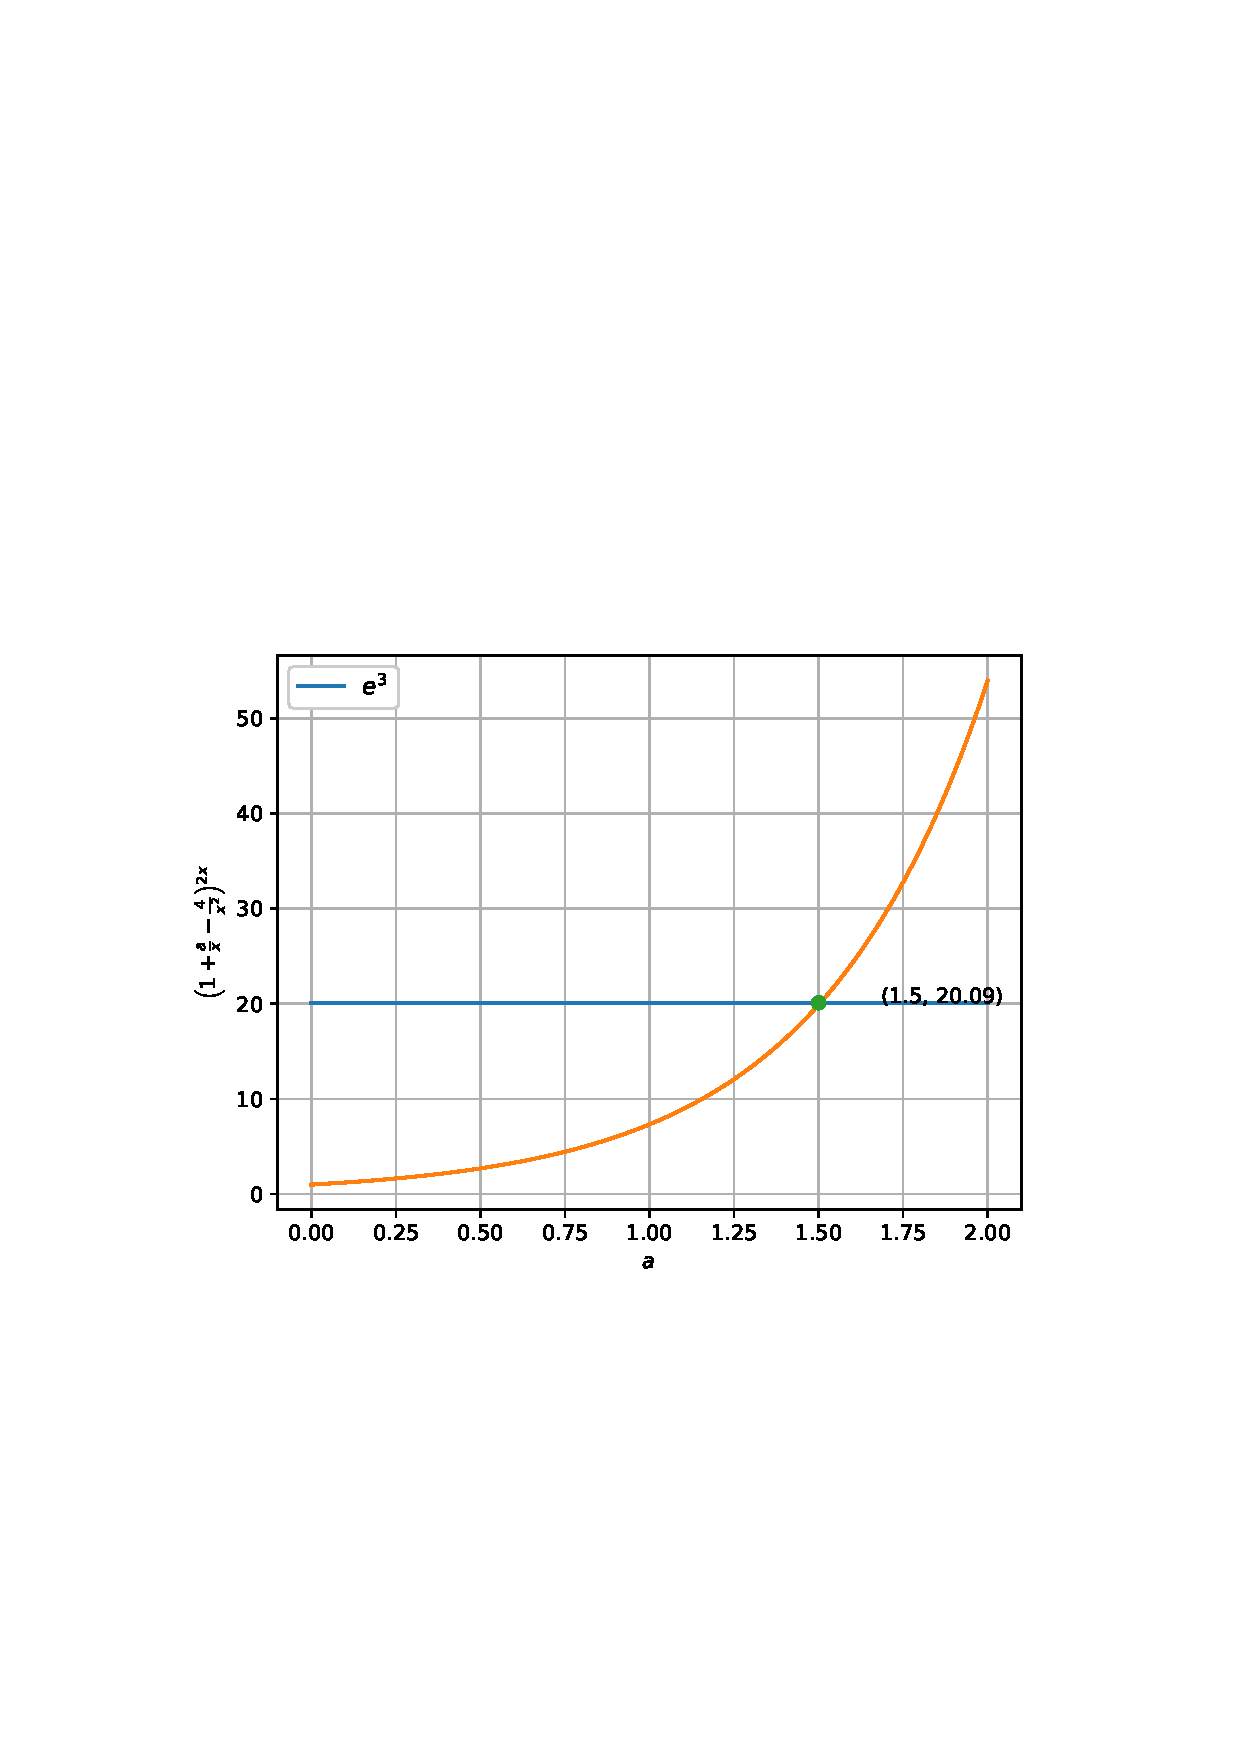
\includegraphics[width=\columnwidth]{./figs/ee16b1004}
\end{center}
\captionof{figure}{LHS and RHS in \eqref{prob_four}}
\label{fig_4}	
\end{figure}
\begin{problem}
The function
%
\begin{equation}
f(x)=
\begin{cases}
-x & x < 1 \\
a + \cos^{-1}\brak{x + b} & 1 \leq x \leq 2
\end{cases}
\end{equation}
%
is known to be differentiable at $x=1$.  What is the value of $\frac{a}{b}$?
\end{problem}
\solution
Since the function is differentiable at $x=1$,
\begin{align}
\label{four_one}
\lim _{ x\rightarrow { 1 }^{ - } }{ f^{ \prime  }\left( x \right)  }  &= \lim _{ x\rightarrow { 1 }^{ + } }{ f^{ \prime  }\left(x \right)  }
\end{align}
Also,
%
\begin{align}
\label{four_two}
 \lim _{ x\rightarrow { 1 }^{ - } }{ f^{ \prime  }\left( x \right)  } &=-1 \\ 
\lim _{ x\rightarrow { 1 }^{ + } }{ f^{ \prime  }\left(x \right)  } &= -\frac { 1 }{ \sqrt { 1-{ (x+b) }^{ 2 } }  } 
\end{align}
%
From \eqref{four_one} and \eqref{four_two},
\begin{align}
-\frac { 1 }{ \sqrt { 1-{ (x+b) }^{ 2 } }} &= -1 \Rightarrow 
b &=-x = -1
\end{align}
Since a differentiable function is also continuous, 
\begin{align}
\lim _{ x\rightarrow { 1 }^{ + } }{ \quad a+\cos ^{ -1 }{ (x+b) }  } &= \lim _{ x\rightarrow { 1 }^{ - } }{ (-x) }  \\
\Rightarrow a+\frac { \pi  }{ 2 } &=-1\\
\Rightarrow a &=-1-\frac { \pi  }{ 2 }
\end{align}
Then
\begin{align}
  c=\frac{a}{b}=1+\frac { \pi  }{ 2 } 
\end{align}


The following python code yields Fig. \ref{fig_5} verifying the above result.
\lstinputlisting{./codes/ee16b1005.py}
\begin{figure}[!ht]
\begin{center}
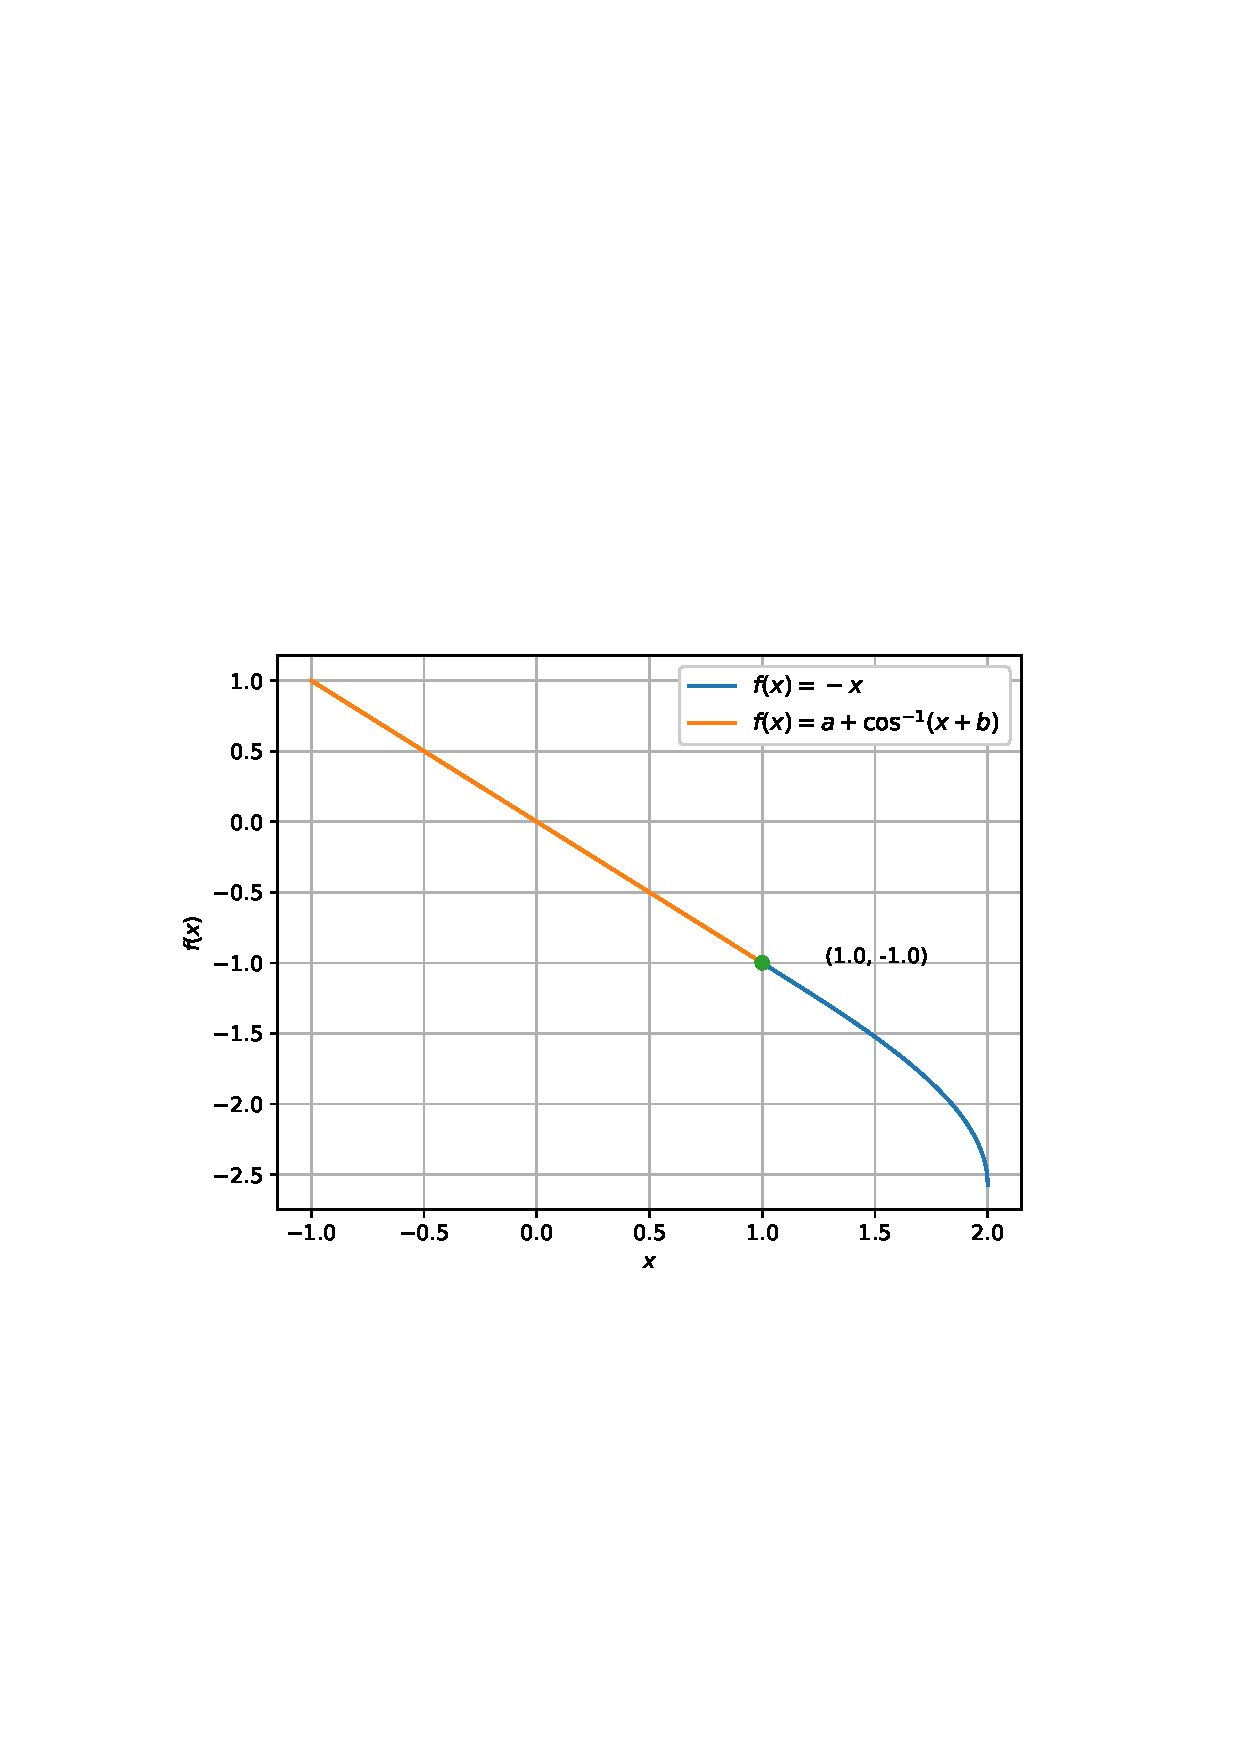
\includegraphics[width=\columnwidth]{./figs/ee16b1005}
\end{center}
\captionof{figure}{Substituting the values of $a$ and $b$ in $f(x)$, the graph is smooth at $x=1$. So $f(x)$ is differentiable $x=1$.}
\label{fig_5}	
\end{figure}
%
\begin{problem}
The tangent at point $P$, for the curve $x = 4t^2+3, y = 8t^3-1$, with parameter $t \in \mathbf{R}$, meets the curve again at $Q$.  Find the coordinates of $Q$.
\end{problem}
\solution 	
Let $P$ and $Q$ be $\brak{4t ^{ 2 }+3, 8 t ^{ 3 }-1}$ and 
 $\brak{4{ { t }_{ 1 } }^{ 2 }+3, 8  {t _{ 1 }} ^ 3 -1}$  respectively.
 At P, 
 \begin{align}
 \frac { dy }{ dx } = \frac { \frac { dy }{ dt } }{ \frac { dx }{ dt } }=\frac{24t^2}{8t}= 3t .
 \end{align}
 Since the tangent at $P$ meets the curve at $Q$, the equation of the tangent can be expressed as
 %
 \begin{align}
 \brak{y - 8t_1^3 +1} = 3t\brak{x - 4t_1^2 - 3}
 \end{align}
 %
 which, upon substitution of coordinates of $P$ yields
%
 \begin{align}
 \brak{8t^3 - 8t_1^3 } &= 3t\brak{4t^2 - 4t_1^2 }
 \\
\Rightarrow 8\brak{t_1 - t}({ { t }_{ 1 } }^{ 2 } + { t }_{ 1 } t + t^2) &= 3t. 4\brak{{ t }_{ 1 }  -t} \brak{{ t }_{ 1 }  + t } \nonumber
\\ 
\Rightarrow 2({ { t }_{ 1 } }^{ 2 }+ { { t }_{ 1 } }t + t^2) &= 3t({ t }_{ 1 }  + t)
 \\ 
\Rightarrow  2{ { t }_{ 1 } }^{ 2 } - t{ { t }_{ 1 } } - t^2 &= 0
\\
\Rightarrow  ({ t }_{ 1 }  - t) (2{ t }_{ 1 }  + t) &= 0
\\
 \Rightarrow  { t }_{ 1 } &= -\frac { t }{ 2 }
 \end{align}
 %
Thus, $Q$ can now be expressed as  $\brak{t^{ 2 }+3, t ^ 3 -1}$.  To demonstrate the solution of this problem, letting $t = 1$, we obtain $P,Q$ as $\brak{7,7},\brak{4,-2}$ respectively and the equation of the tangent is
%
\begin{align}
y-7 = 3\brak{x - 7}
\end{align}
%


The following code generates the plot in Fig. \ref{fig_6} for this problem. 
\lstinputlisting{./codes/ee16b1006.py}
\begin{figure}[!ht]
\begin{center}
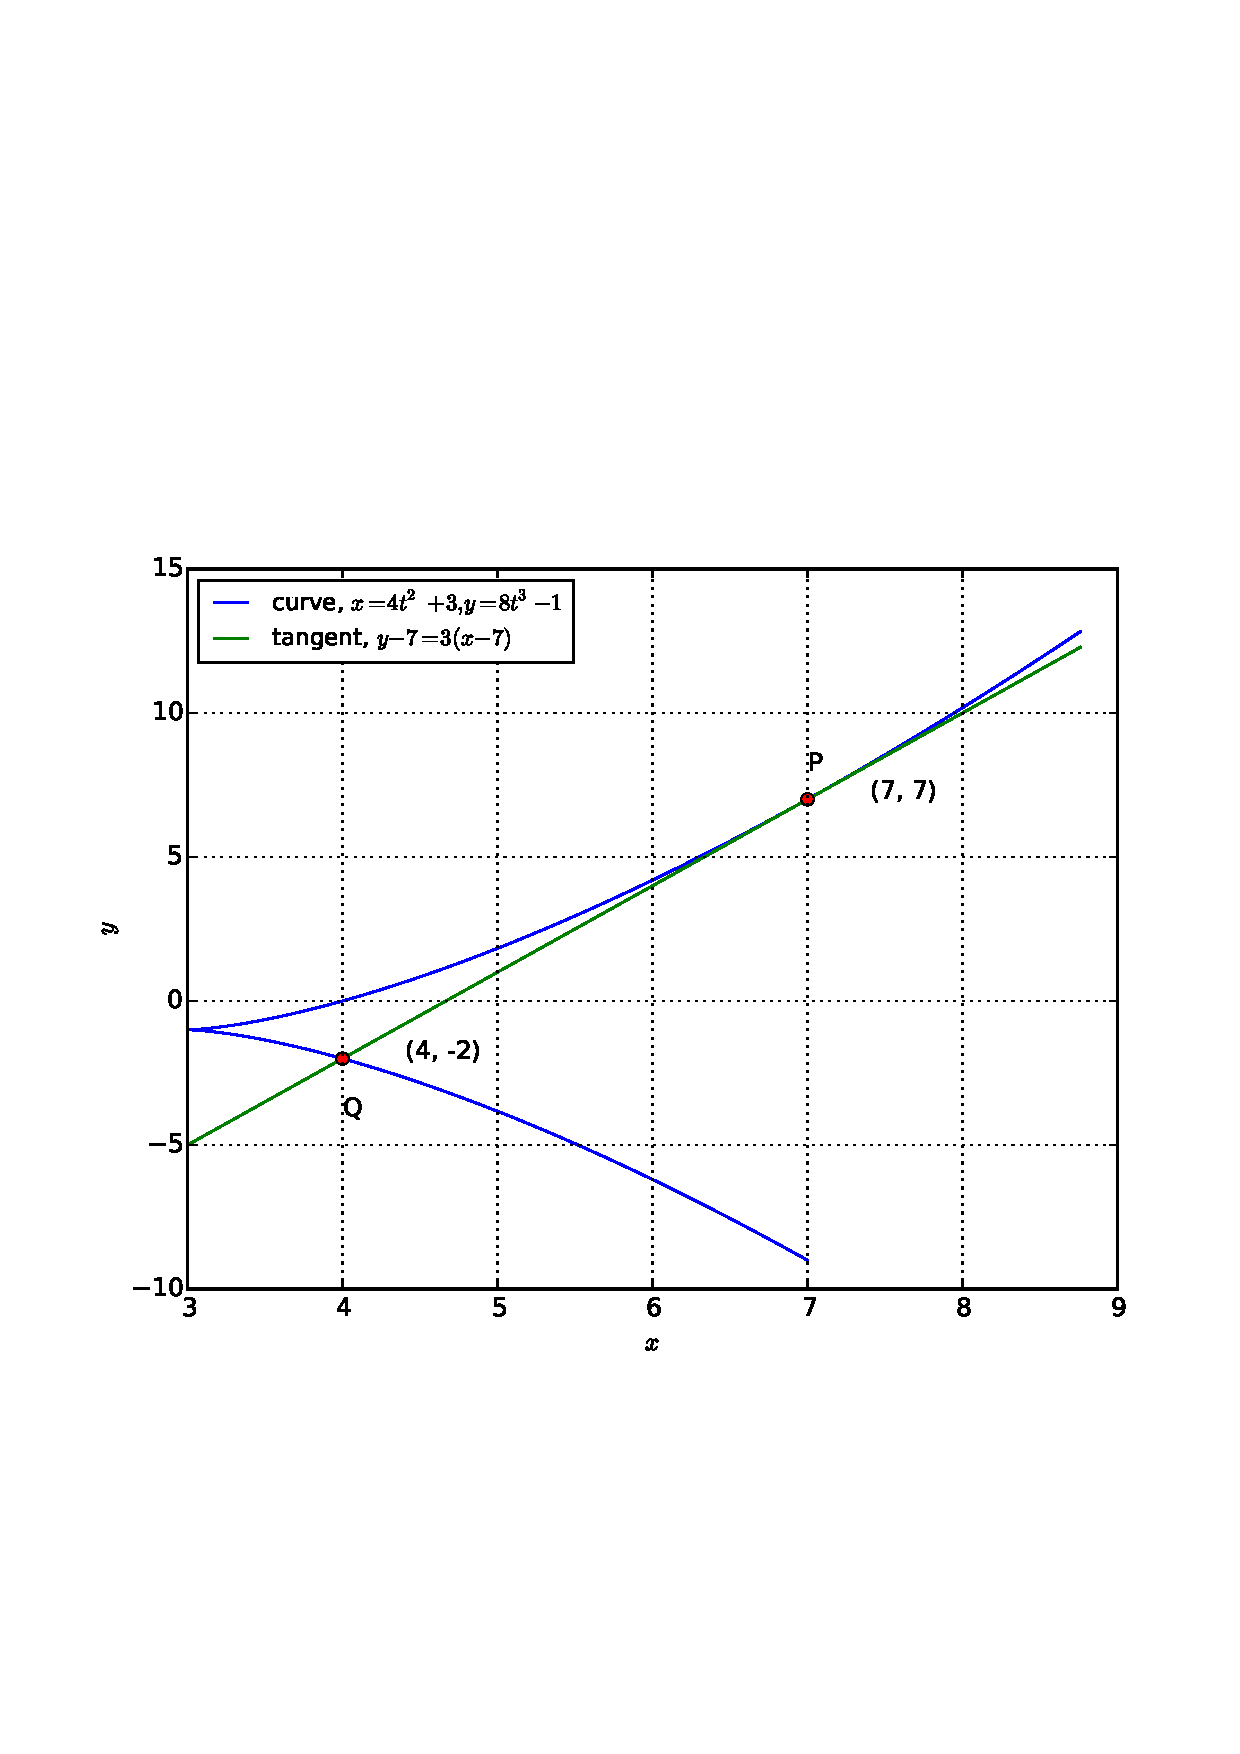
\includegraphics[width=\columnwidth]{./figs/ee16b1006}
\end{center}
\captionof{figure}{The tangent at $P$ meets the curve again at $Q$.}
\label{fig_6}	
\end{figure}
%
\begin{problem}
Find the minimum distance of a point on the curve $y = x^2 -4$ from the origin.
\end{problem}
\solution
Let P be the  point on the curve closest to the origin. If the coordinates of the the point be $\brak{h,k}$, then its  distance from the origin is given by
%
\begin{equation}
\label{seven_dist}
d^2 = h^2+k^2
\end{equation}
%
Since $P$ lies on the curve, 
%
\begin{equation}
\label{seven_def}
k = h^2-4
\end{equation}
%
From \eqref{seven_dist} and \eqref{seven_def},
%
\begin{align}
\label{seven_min}
d^2 &= k^2+k+4 \nonumber \\
&= \brak{k + \frac{1}{2}}^2 +\frac{15}{4}
\end{align}
%
Thus, the smallest distance is given by the above equation as $\frac{\sqrt{15}}{2}$. The nearest point is given by \eqref{seven_def} and \eqref{seven_min} as $\brak{\pm \sqrt{\frac{7}{2}},-\frac{1}{2}}$

%\end{document}

The following code yields Figs. \ref{fig_7a} and \ref{fig_7b} explaining the solution.
\lstinputlisting{./codes/ee16b1007.py}
\renewcommand{\thefigure}{\theproblem.\arabic{figure}}

\begin{figure}[!h]
\begin{center}
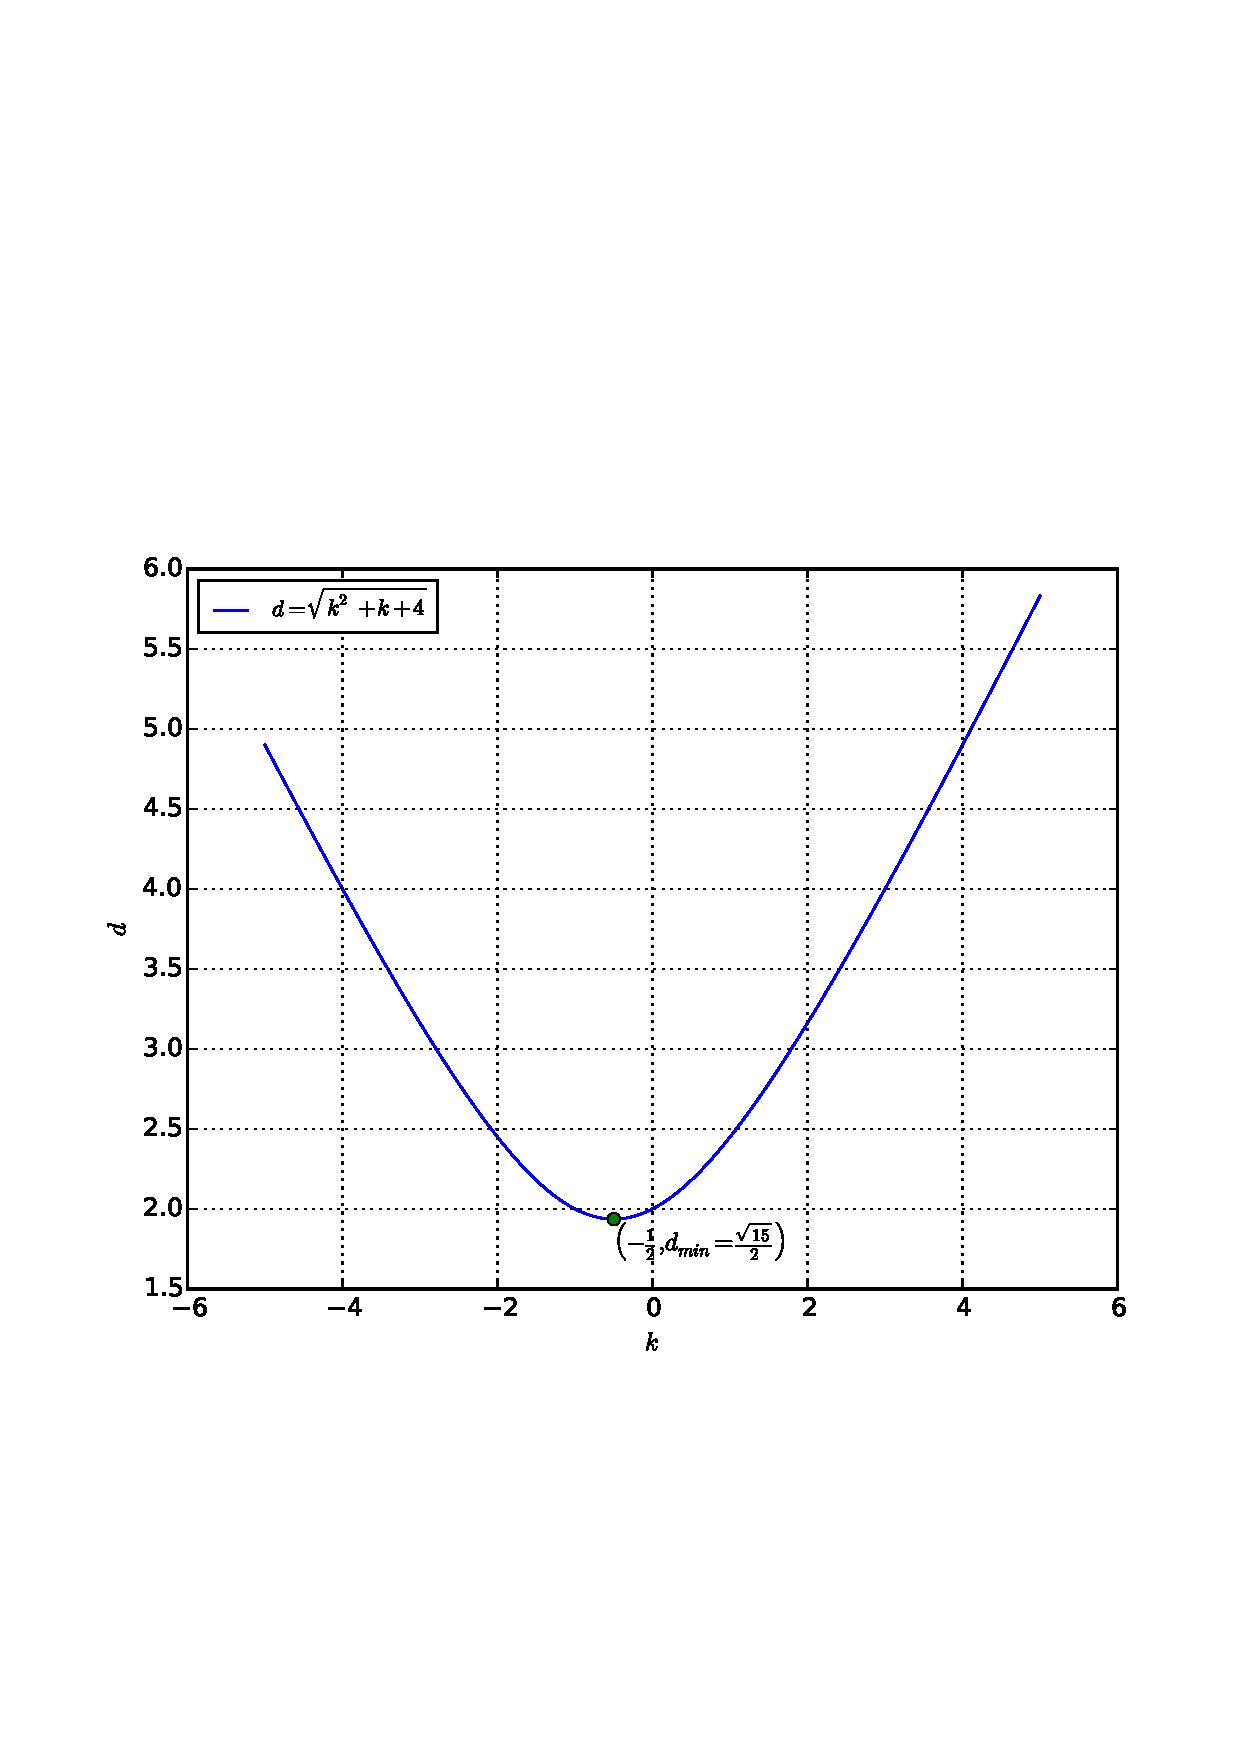
\includegraphics[width=\columnwidth]{./figs/ee16b1007a}
\end{center}
\captionof{figure}{The minimum distance is $\frac{\sqrt{17}}{2}$ for $k = -\frac{1}{2}$}
\label{fig_7a}	
\end{figure}
%
\begin{figure}[!h]
\begin{center}
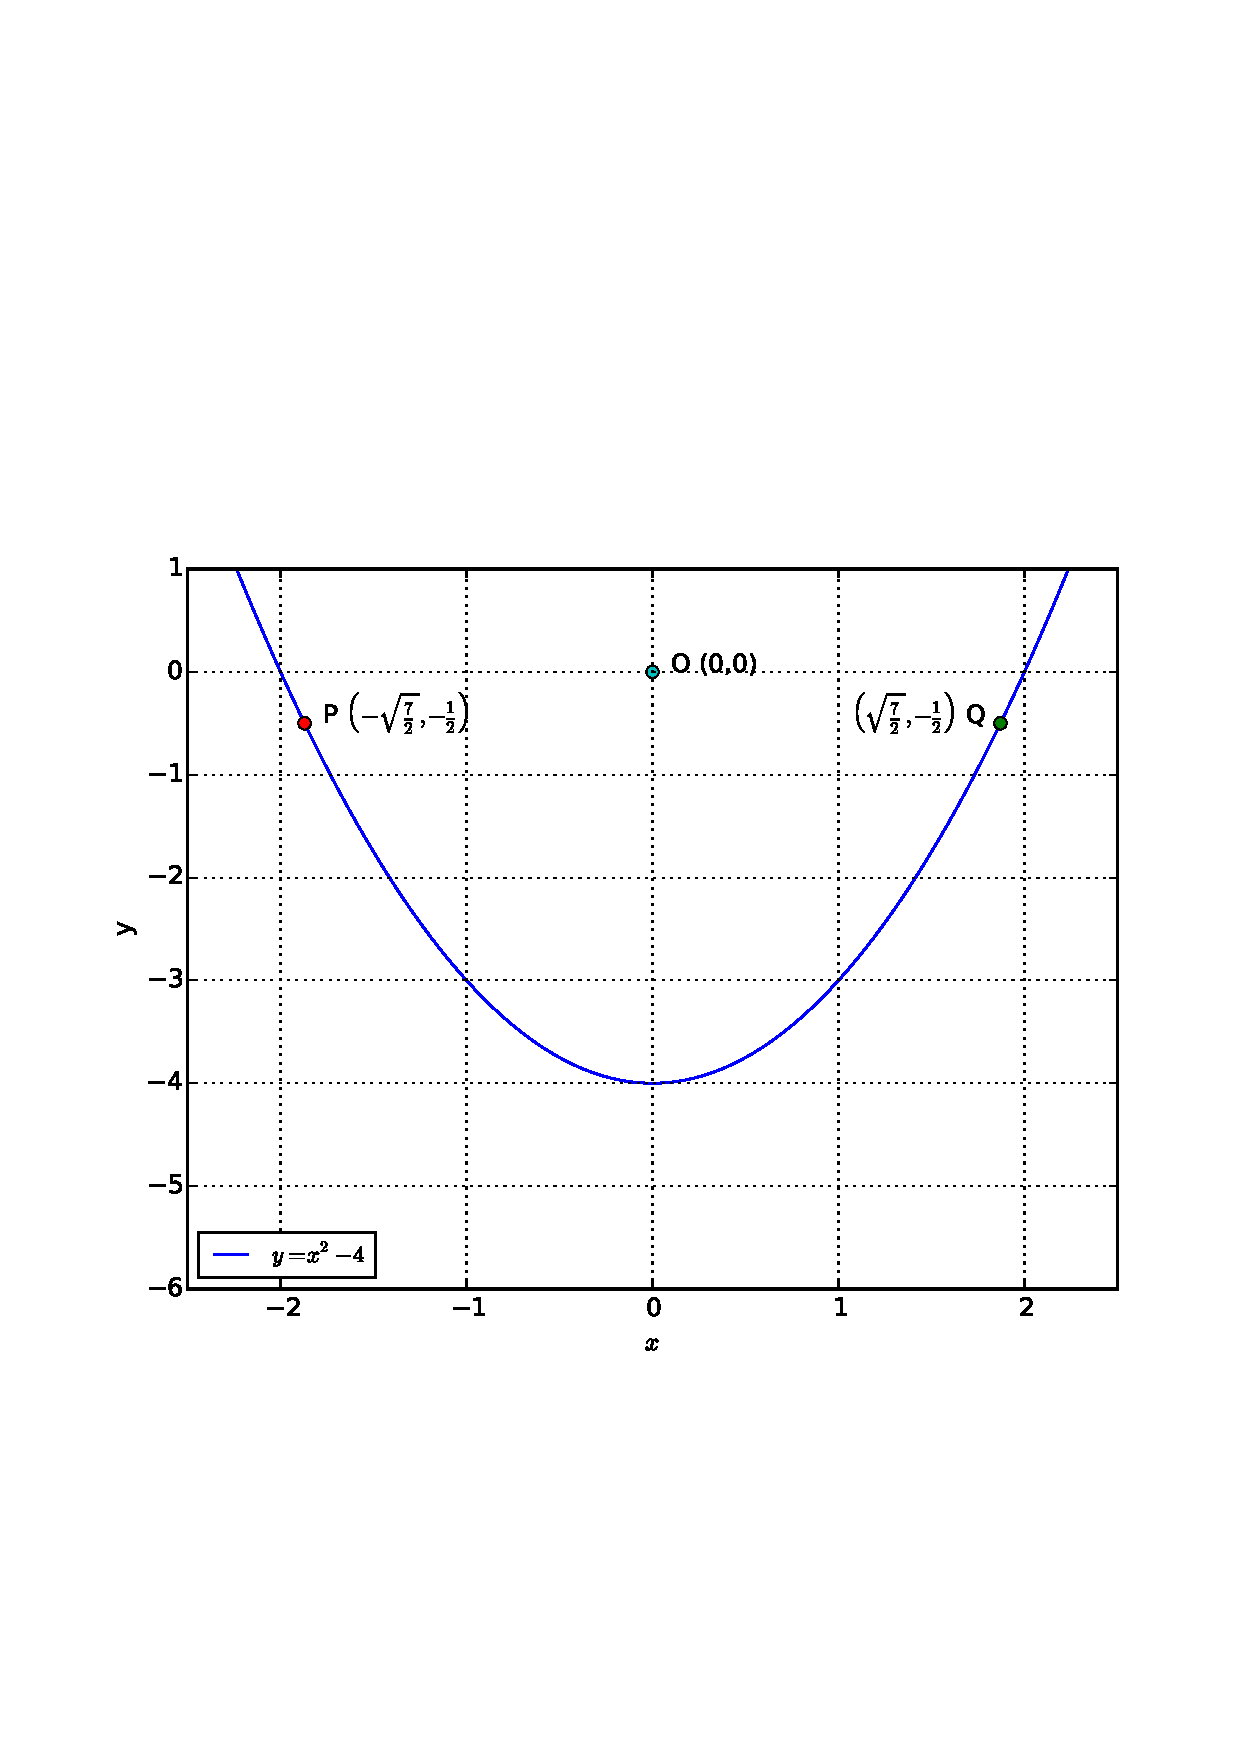
\includegraphics[width=\columnwidth]{./figs/ee16b1007b}
\end{center}
\captionof{figure}{$OP$ and $OQ$ represent the minimum distance of the origin from the parabola.}
\label{fig_7b}	
\end{figure}
\renewcommand{\thefigure}{\theproblem}
\begin{problem}
Sketch the region
\begin{equation}
A = \cbrak{\brak{x,y}\vert y \geq x^2-5x+4, x + y \geq 1, y \leq 0}.
\end{equation}
%
\end{problem}
\solution The desired region is plotted in Fig. \ref{fig_8} using the following code.
\lstinputlisting{./codes/ee16b1008.py}
\begin{figure}
\begin{center}
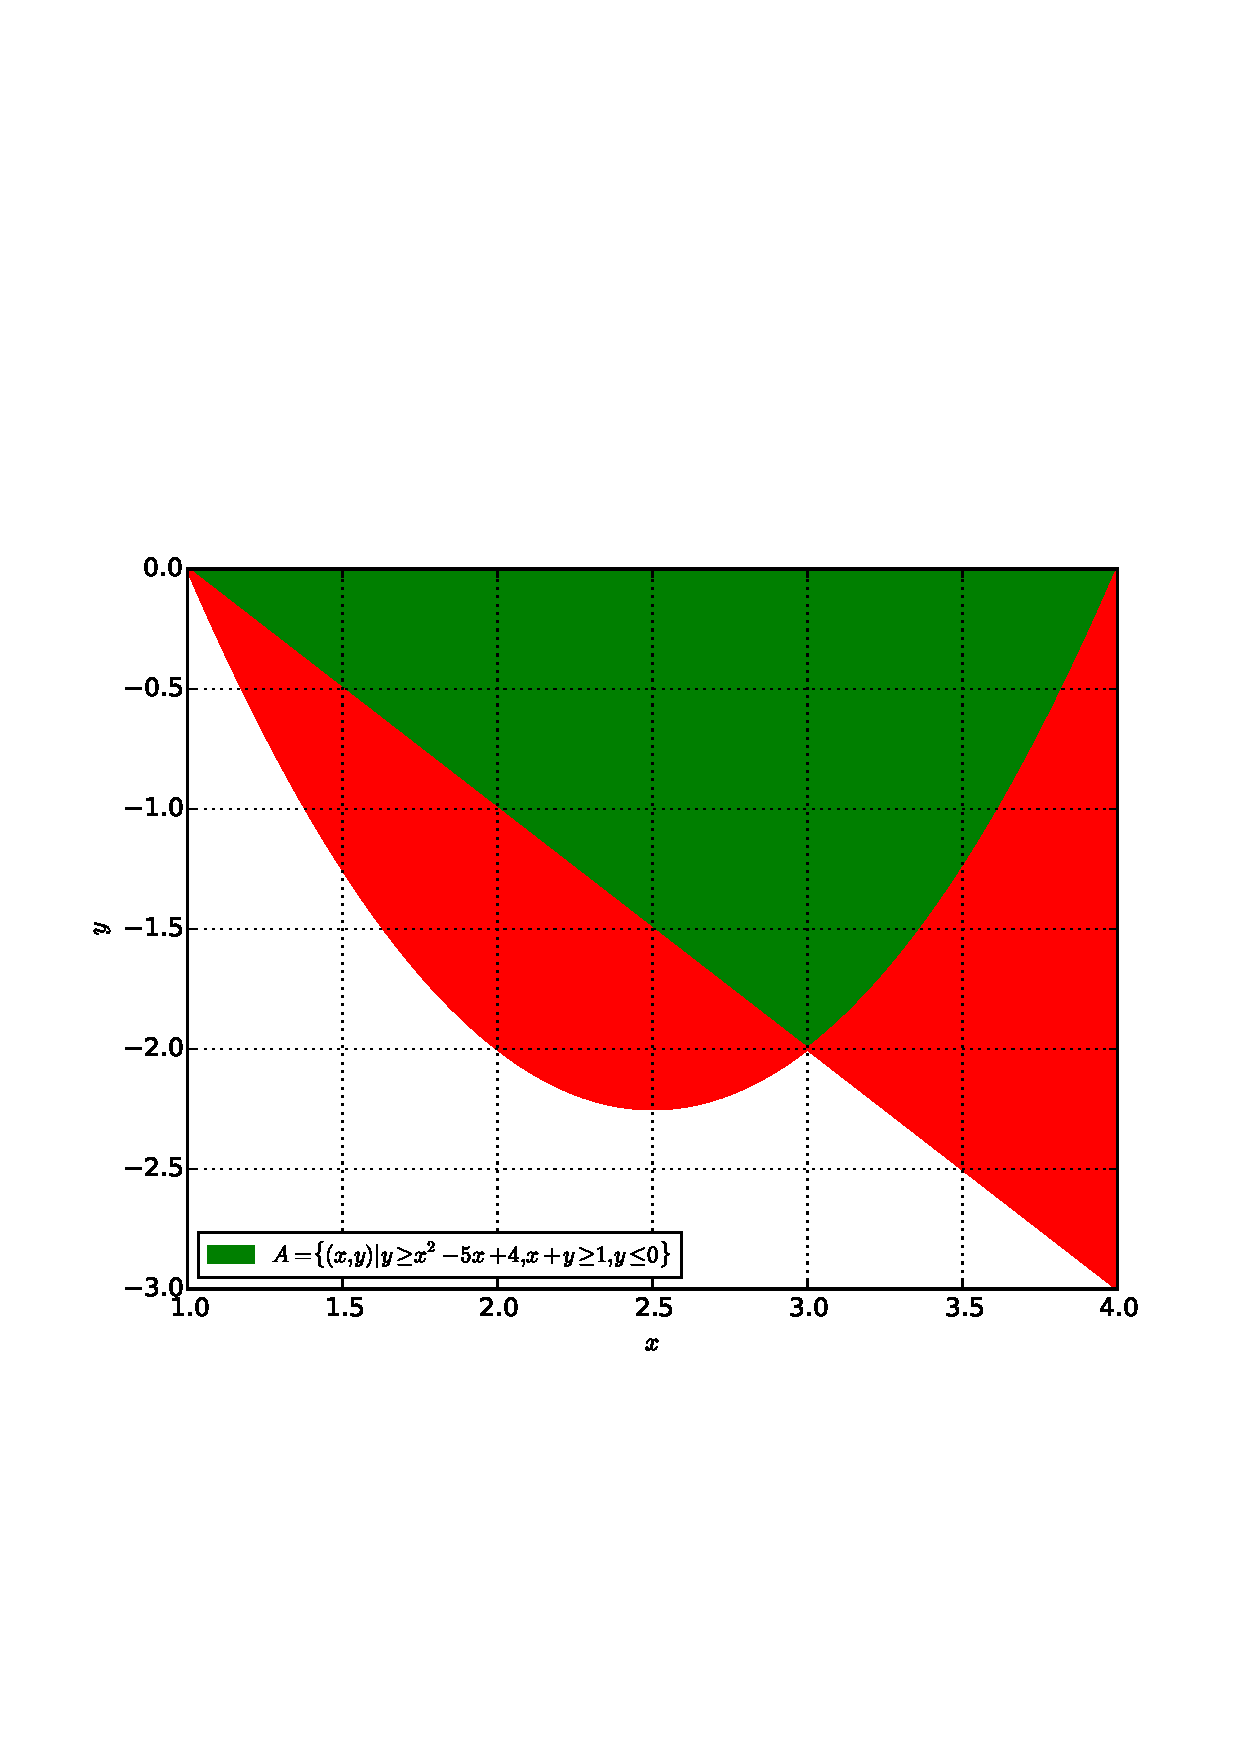
\includegraphics[width=\columnwidth]{./figs/ee16b1008}
\end{center}
\captionof{figure}{The desired region is in green colour.}
\label{fig_8}	
\end{figure}
%
\begin{problem}
A variable line drawn through the intersection of the lines $\frac{x}{3} + \frac{y}{4} = 1$ and $\frac{x}{4} + \frac{y}{3} = 1$ meets the coordinate axes at $A$ and $B, A \neq B$.  Sketch the locus of the midpoint of $AB$.
\end{problem}
\solution
The interstion of the two lines is the solution of the matrix equation
%
\begin{equation}
\begin{pmatrix}
\frac{1}{3} & \frac{1}{4} \\
\frac{1}{4} & \frac{1}{3}
\end{pmatrix}
\begin{pmatrix}
x\\
y
\end{pmatrix}
=
\begin{pmatrix}
1
\\
1
\end{pmatrix}
\end{equation}
%
given by $\brak{\frac{12}{7},\frac{12}{7}}$. 
If $A$  is $(a,0)$ and $B$ is $(0,b)$, the mid point of $AB$ is $\brak{\frac{a}{2},\frac{b}{2}}$. The equation of the line $AB$ is
%
\begin{equation}
\frac{x}{a} + \frac{y}{b} = 1
\end{equation}
%
From the given information, this line passes through $\brak{\frac{12}{7},\frac{12}{7}}$.  Substituting $h = \frac{a}{2}, y = \frac{b}{2}$ in the above and simplifying, the locus is obtained as
%
\begin{align}
\frac{1}{h} + \frac{1}{k} = \frac{7}{6}
\end{align}
%

The sketch of the locus is available in Fig. \ref{fig_9}.
\lstinputlisting{./codes/ee16b1009.py}
\begin{figure}
\begin{center}
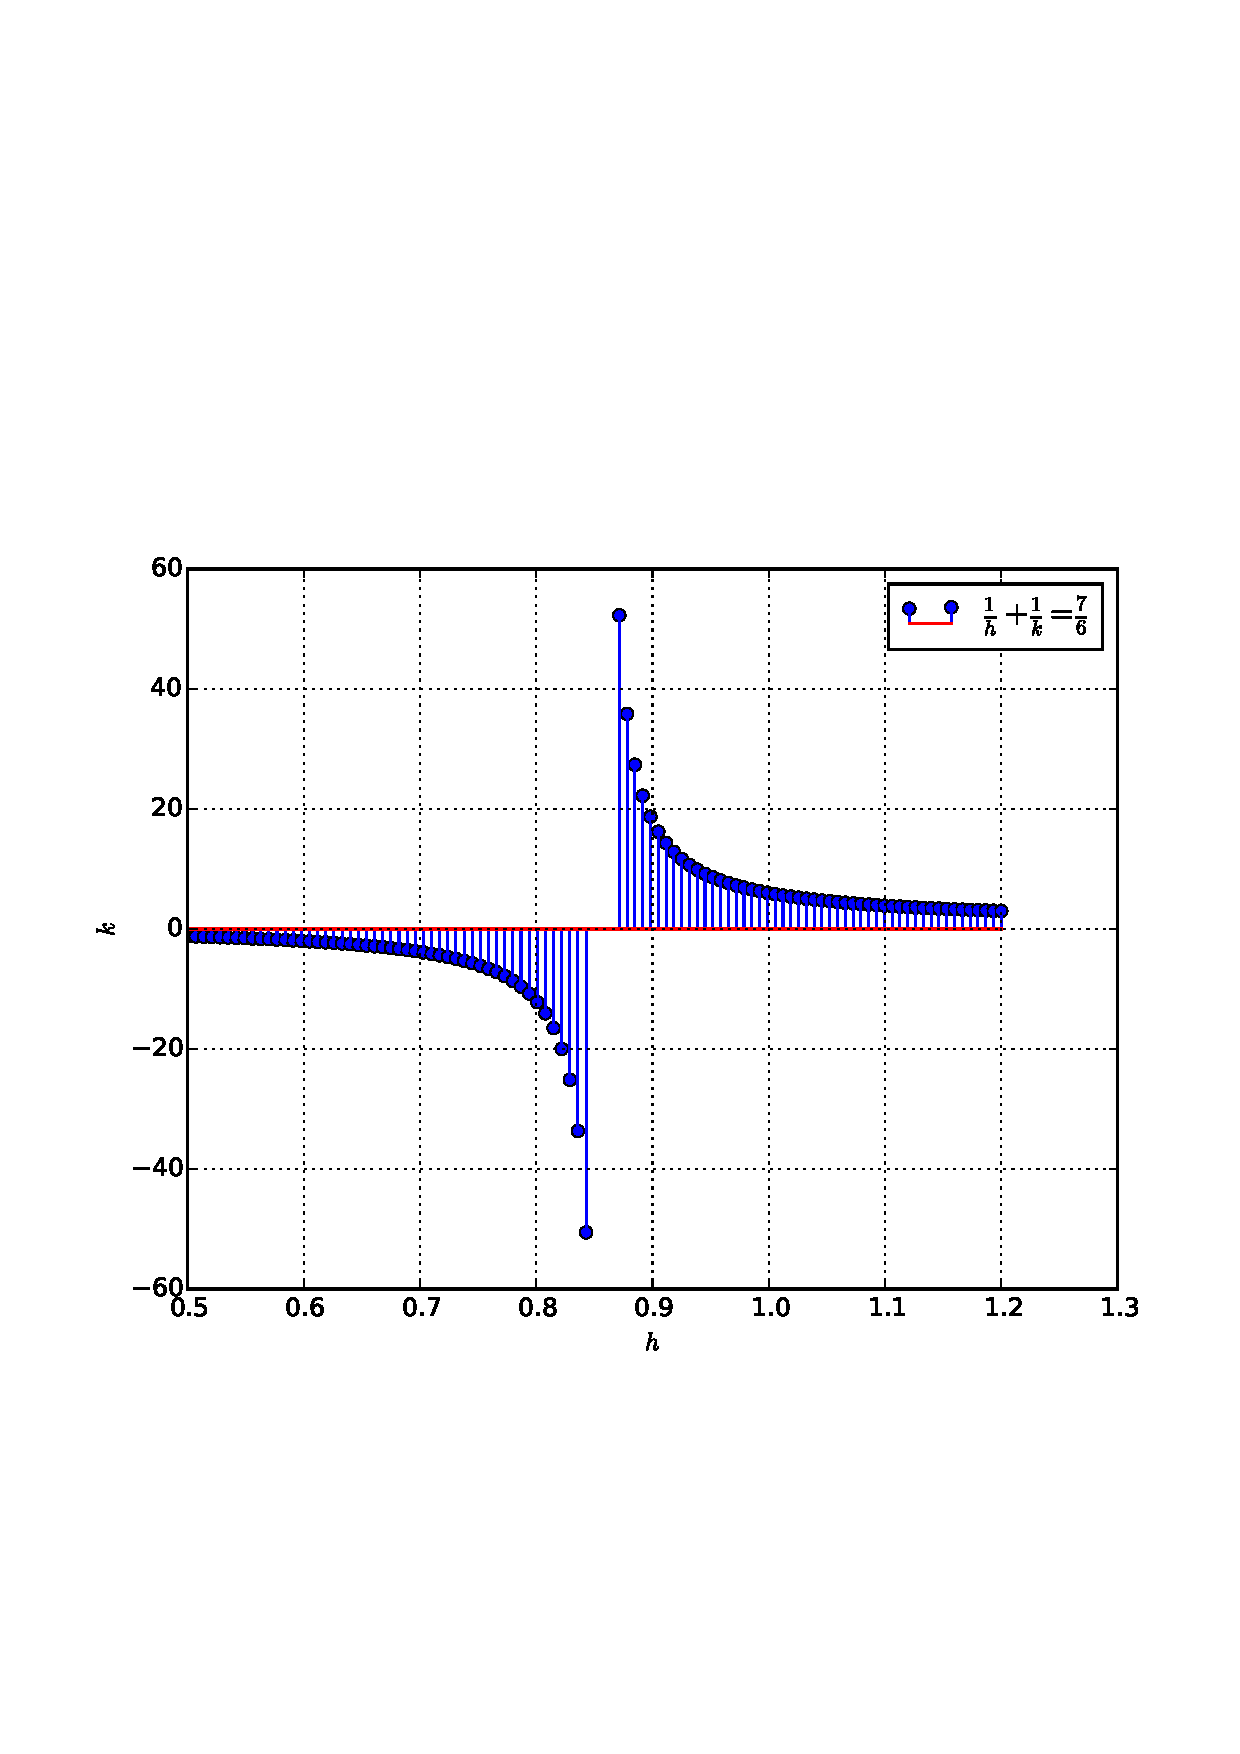
\includegraphics[width=\columnwidth]{./figs/ee16b1009}
\end{center}
\captionof{figure}{Locus of the midpoint. Symmetric about the the point $\brak{\frac{6}{7},0}$}
\label{fig_9}	
\end{figure}
%
\begin{problem}
The point $\brak{2,1}$ is translated parallel to the line $L:x-y=4$ by $2\sqrt{3}$ units to yield the point $Q$.  If $Q$ lies in the 3rd quadrant, 
sketch the line passing through $Q$ and $\perp$ L.
\end{problem}
%
\solution
The slope of the given line is $1$ indicating an angle of $\frac{\pi}{4}$. Thus, the coordinates of $Q$ are 
%
\begin{equation}
\brak{2 - 2\sqrt{3}\cos \frac{\pi}{4}, 1 - 2\sqrt{3}\frac{\pi}{4}} = \brak{2 - \sqrt{6}, 1 - \sqrt{6}}
\end{equation}
%
The equation of the line perpendicular to $L$ can be expressed as
%
\begin{equation}
x+y =c
\end{equation}
%
Since this line passes through $Q$, $c = 3 - 2\sqrt{6}$.


Fig. \ref{fig_10} illustrates this problem.
\lstinputlisting{./codes/ee16b1010.py}
\begin{figure}
\begin{center}
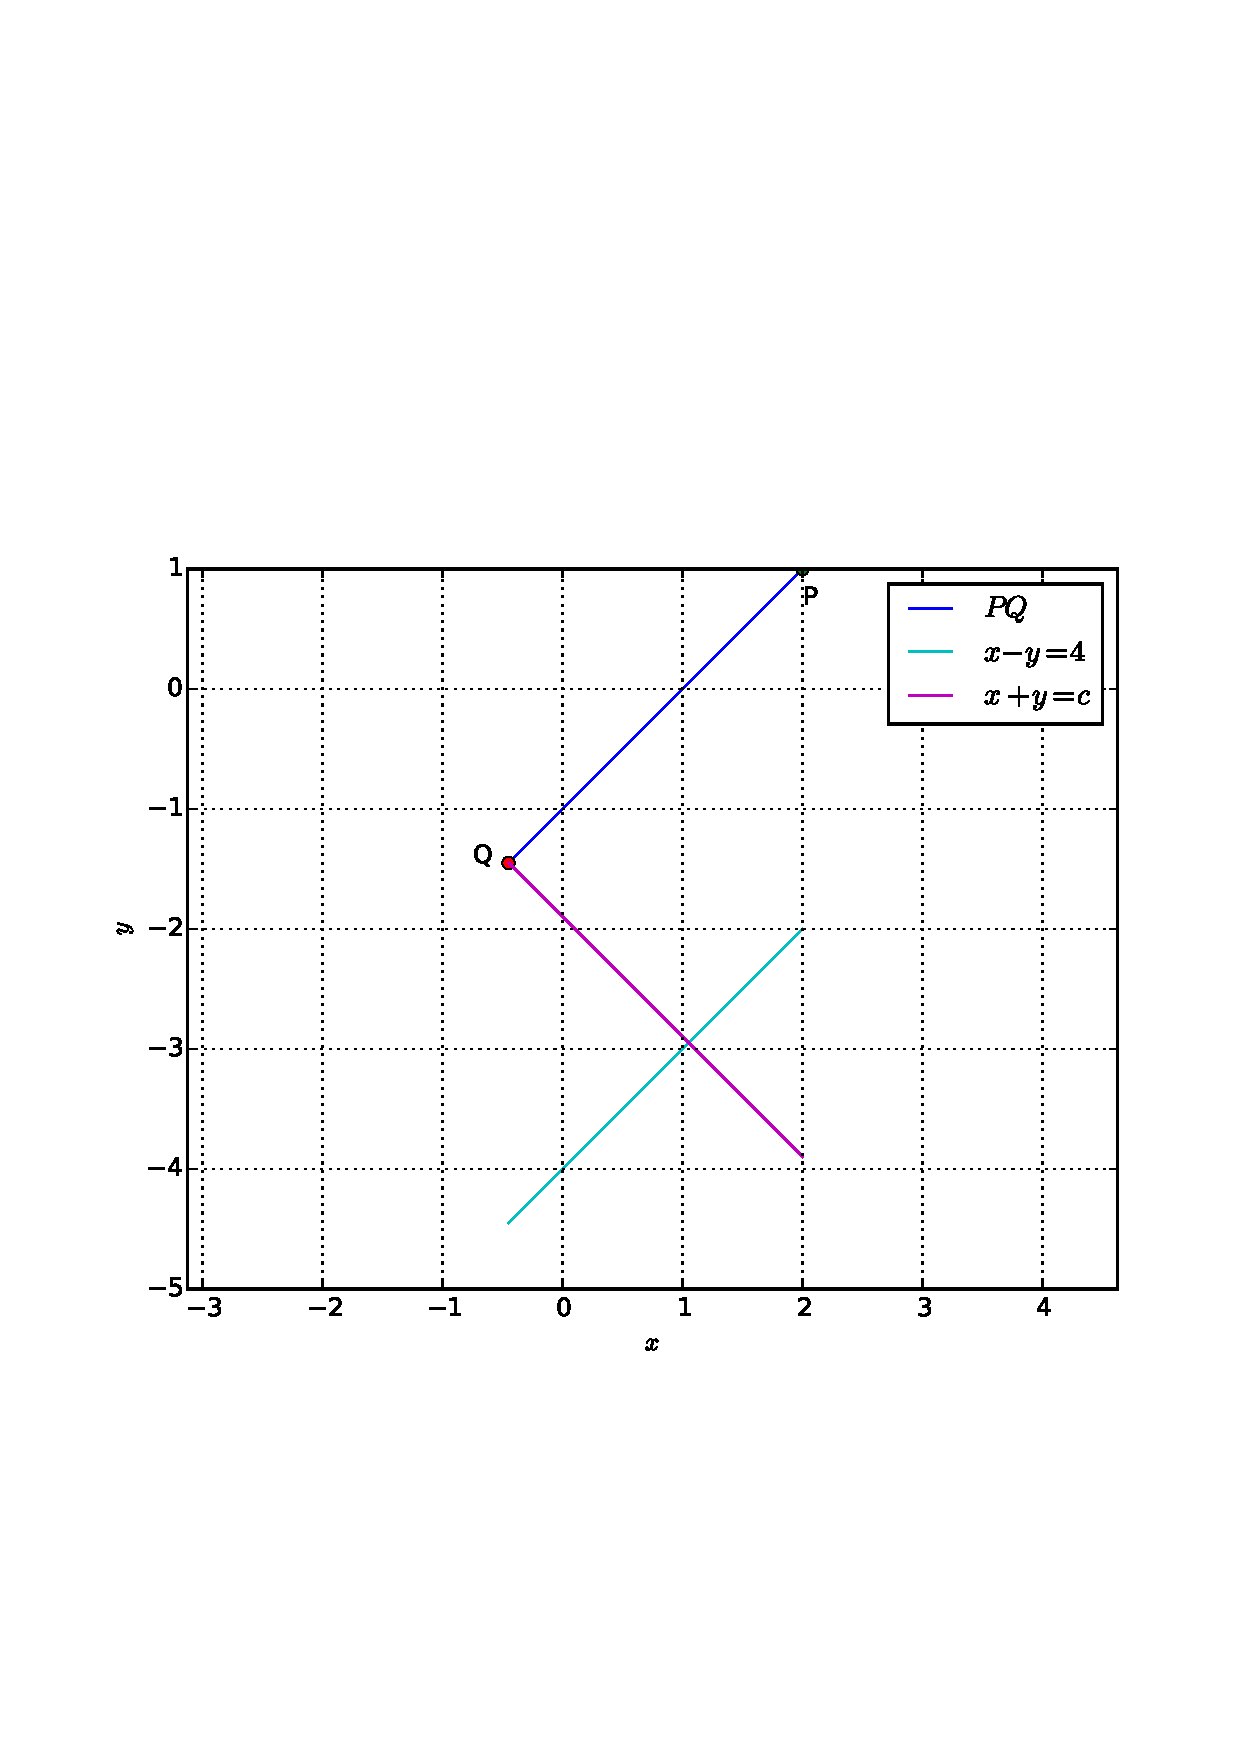
\includegraphics[width=\columnwidth]{./figs/ee16b1010}
\end{center}
\captionof{figure}{$c = 3 - 2\sqrt{6}$}
\label{fig_10}	
\end{figure}
%

\begin{problem}
A circle passes through $\brak{-2,4}$ and touches the $y-$axis at $\brak{0,2}$. Find out which of the following lines represents the diameter of the circle.
\begin{enumerate}
\item $4x+5y-6=0$
\item $2x-3y +10 = 0$
\item $3x+4y-3 = 0$
\item $5x+2y+4 = 0$
\end{enumerate}
\end{problem}
%
\solution
Let the equation of the circle be
%
\begin{equation}
\brak{x-h}^2 + \brak{y-k}^2 = r^2
\end{equation}
%
Since the circle touches the $y$-axis, the radius of the circle is $\abs{h}$ and $k = 2$.  Thus, the equation of the circle can be
expressed as
%
\begin{equation}
\brak{x-h}^2 + \brak{y-2}^2 = h^2
\end{equation}
%
Since the circle passes through the points  $\brak{-2,4}$, substituting these in the above equation yields
%
\begin{align}
\brak{h+2}^2 + 4 &= h^2 \\
\Rightarrow h = -2
\end{align}
%
Thus, the equation of the circle is
%
\begin{equation}
\brak{x+2}^2 + \brak{y-2}^2 = 4
\end{equation}
%

Fig. \ref{fig_11} illustrates this problem.
\lstinputlisting{./codes/ee16b1011.py}
\begin{figure}
\begin{center}
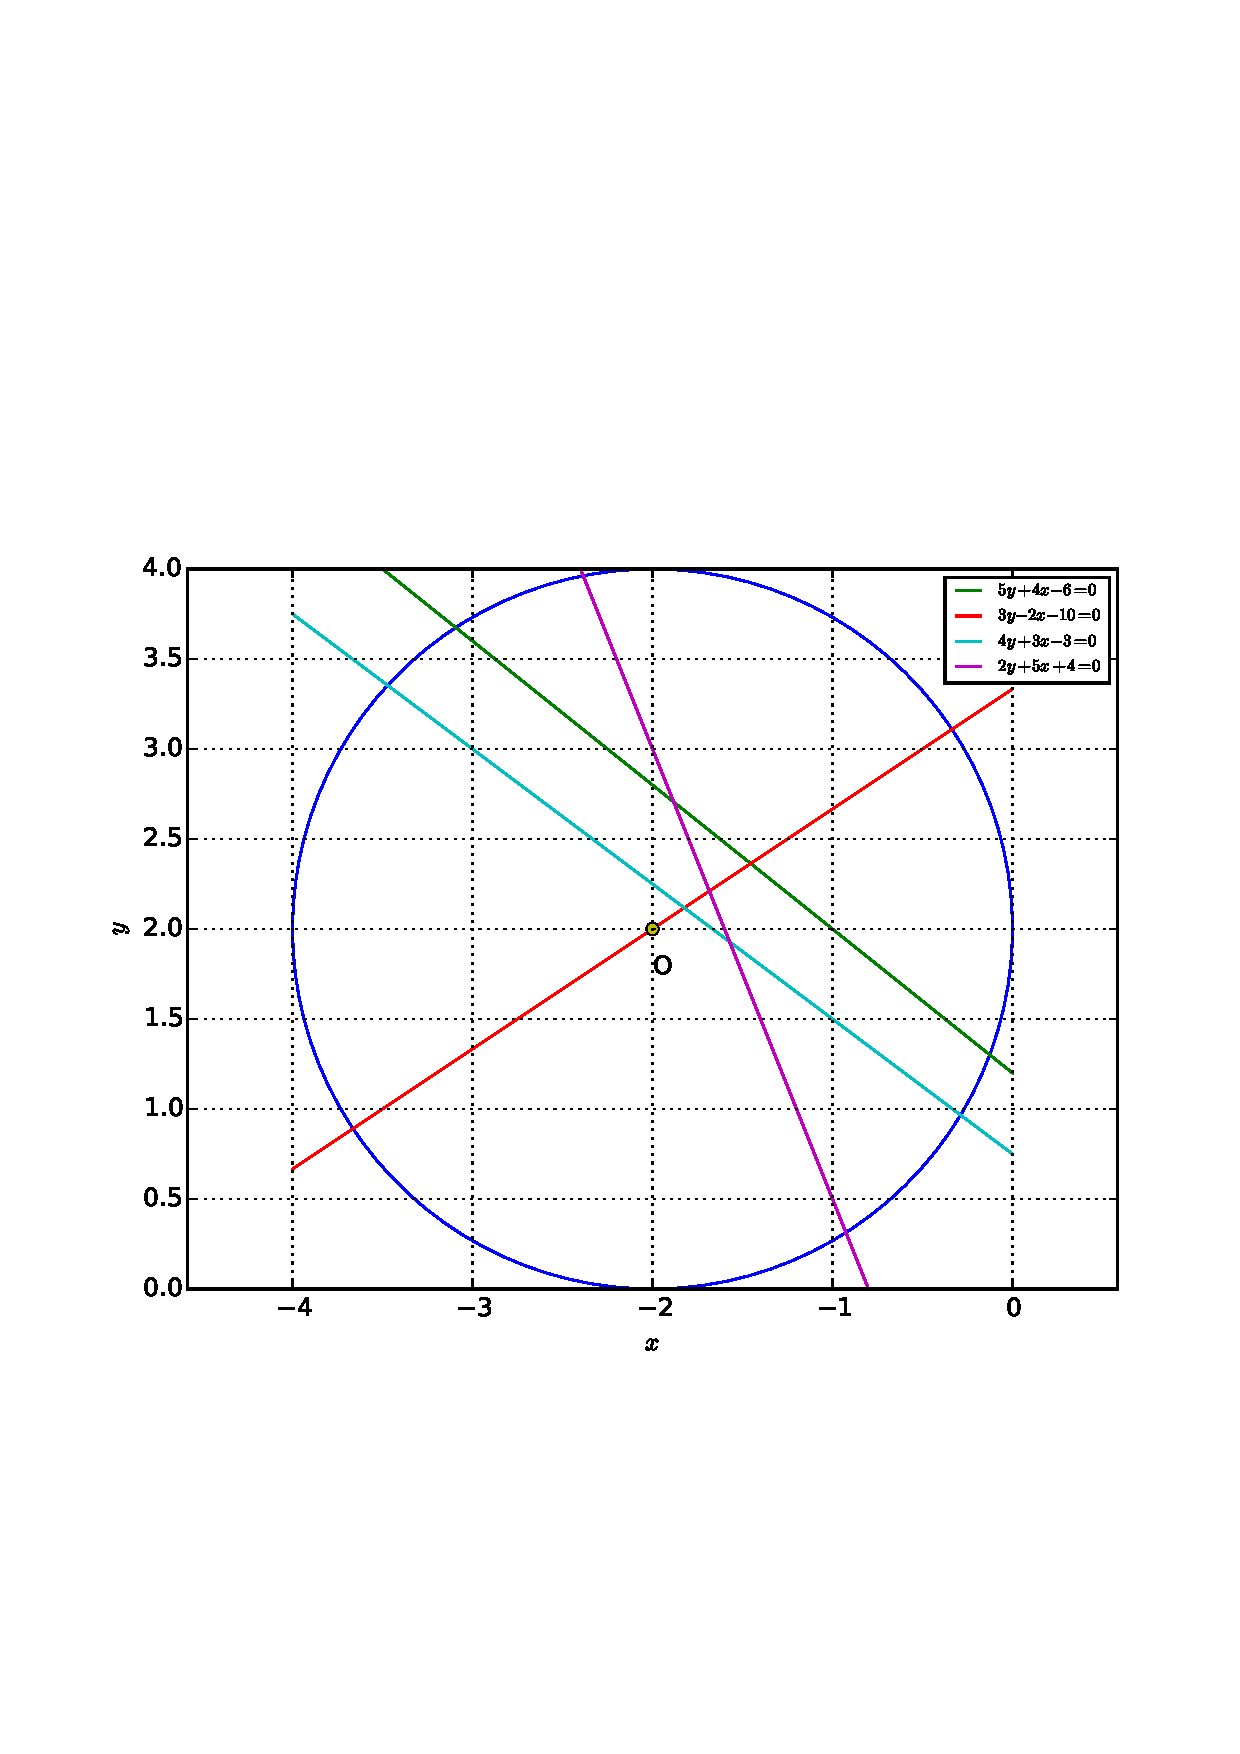
\includegraphics[width=\columnwidth]{./figs/ee16b1011}
\end{center}
\captionof{figure}{$2x-3y +10 = 0$ is the diameter.}
\label{fig_11}	
\end{figure}
%
\begin{problem}
The eccentricity of a hyperbola satisfies the equation $9e^2-18e+5 = 0$. $\brak{5,0}$ is a focus and the corresponding directrix is $5x = 9$. Plot the hyperbola.
\end{problem}
%
\solution
The standard equation of hyperbola 
\begin{equation}
\frac{x^2}{a^2}-\frac{y^2}{b^2}=1
\end{equation}
%
and the eccentricity is given by
\begin{equation}
\label{twelve_eab}
e^2 = 1 + \frac{b^2}{a^2}
\end{equation}             
%
The focus of the hyperbola is at $(ae,0), e > 1$.  From the given information,             
%
\begin{align}
             9e^2-18e+5&=0 ,\\
          \Rightarrow      (3e-1)(3e-5)&=0\\
\end{align}
%
yielding $e=\frac{1}{3}$ or $e=\frac{5}{3}$.  Since $e > 1$, the desired value of the eccentricity is $e = \frac{5}{3}$.  Since the focus is at $\brak{5,0}$, $a = 3$. From \eqref{twelve_eab}, substituting for the values of $a$ and $e$,
%
\begin{align}
1 + \brak{\frac{b}{3}}^2 &= \brak{\frac{5}{3}}^2. \\
\Rightarrow b &=4
\end{align}
%
Thus, the equation of the parabola is
\begin{equation}
\frac{x^2}{9}-\frac{y^2}{16}=1
\end{equation}

%
The following code plots the hyperbola in Fig. \ref{fig_12}.
\lstinputlisting{./codes/ee16b1012.py}
\begin{figure}
\begin{center}
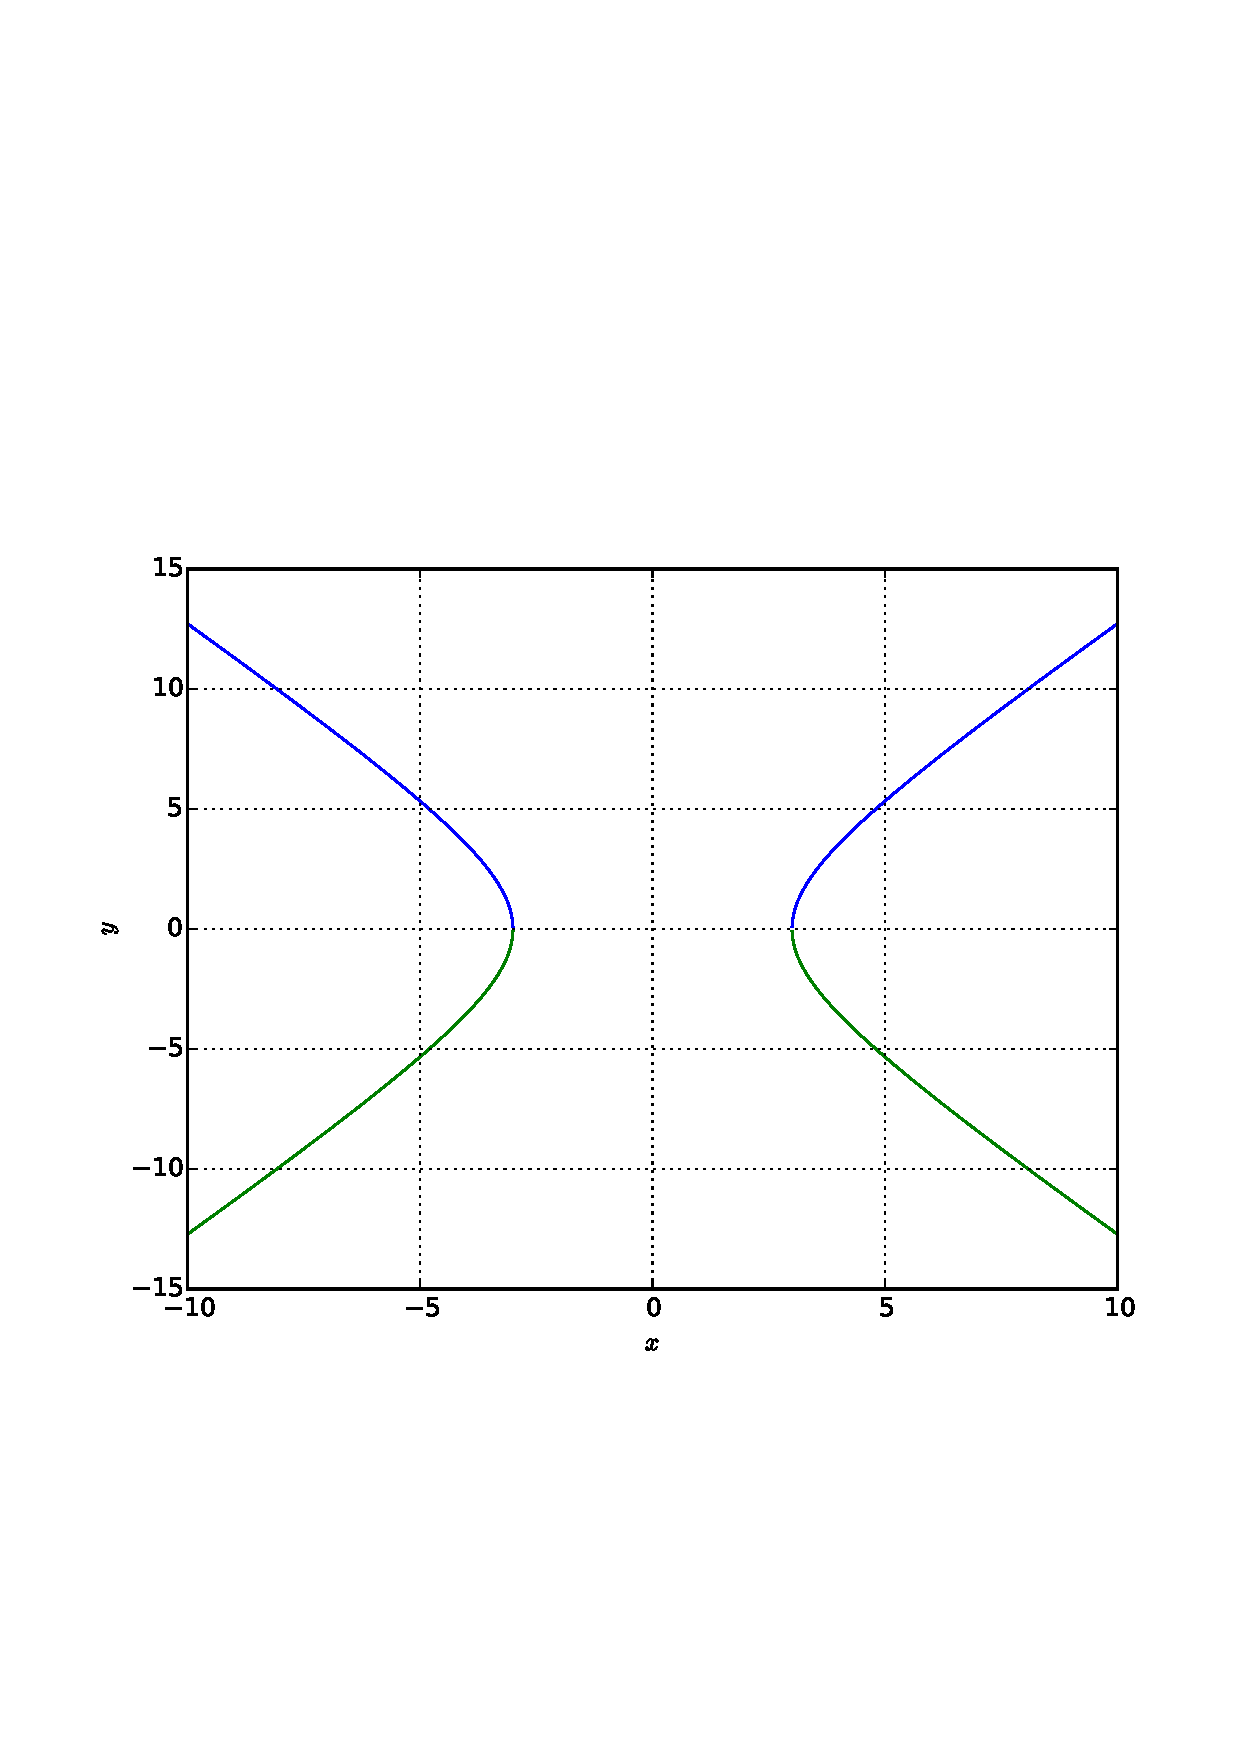
\includegraphics[width=\columnwidth]{./figs/ee16b1012}
\end{center}
\captionof{figure}{Sketch of the hyperbola}
\label{fig_12}	
\end{figure}
%
\begin{problem}
Sketch the ellipse $\frac{x^2}{27} + \frac{y^2}{3} = 1$.
\end{problem}
\solution The following code plots the ellipse in Fig. \ref{fig_13}
\lstinputlisting{./codes/ee16b1013.py}
\begin{figure}[h]
\centering
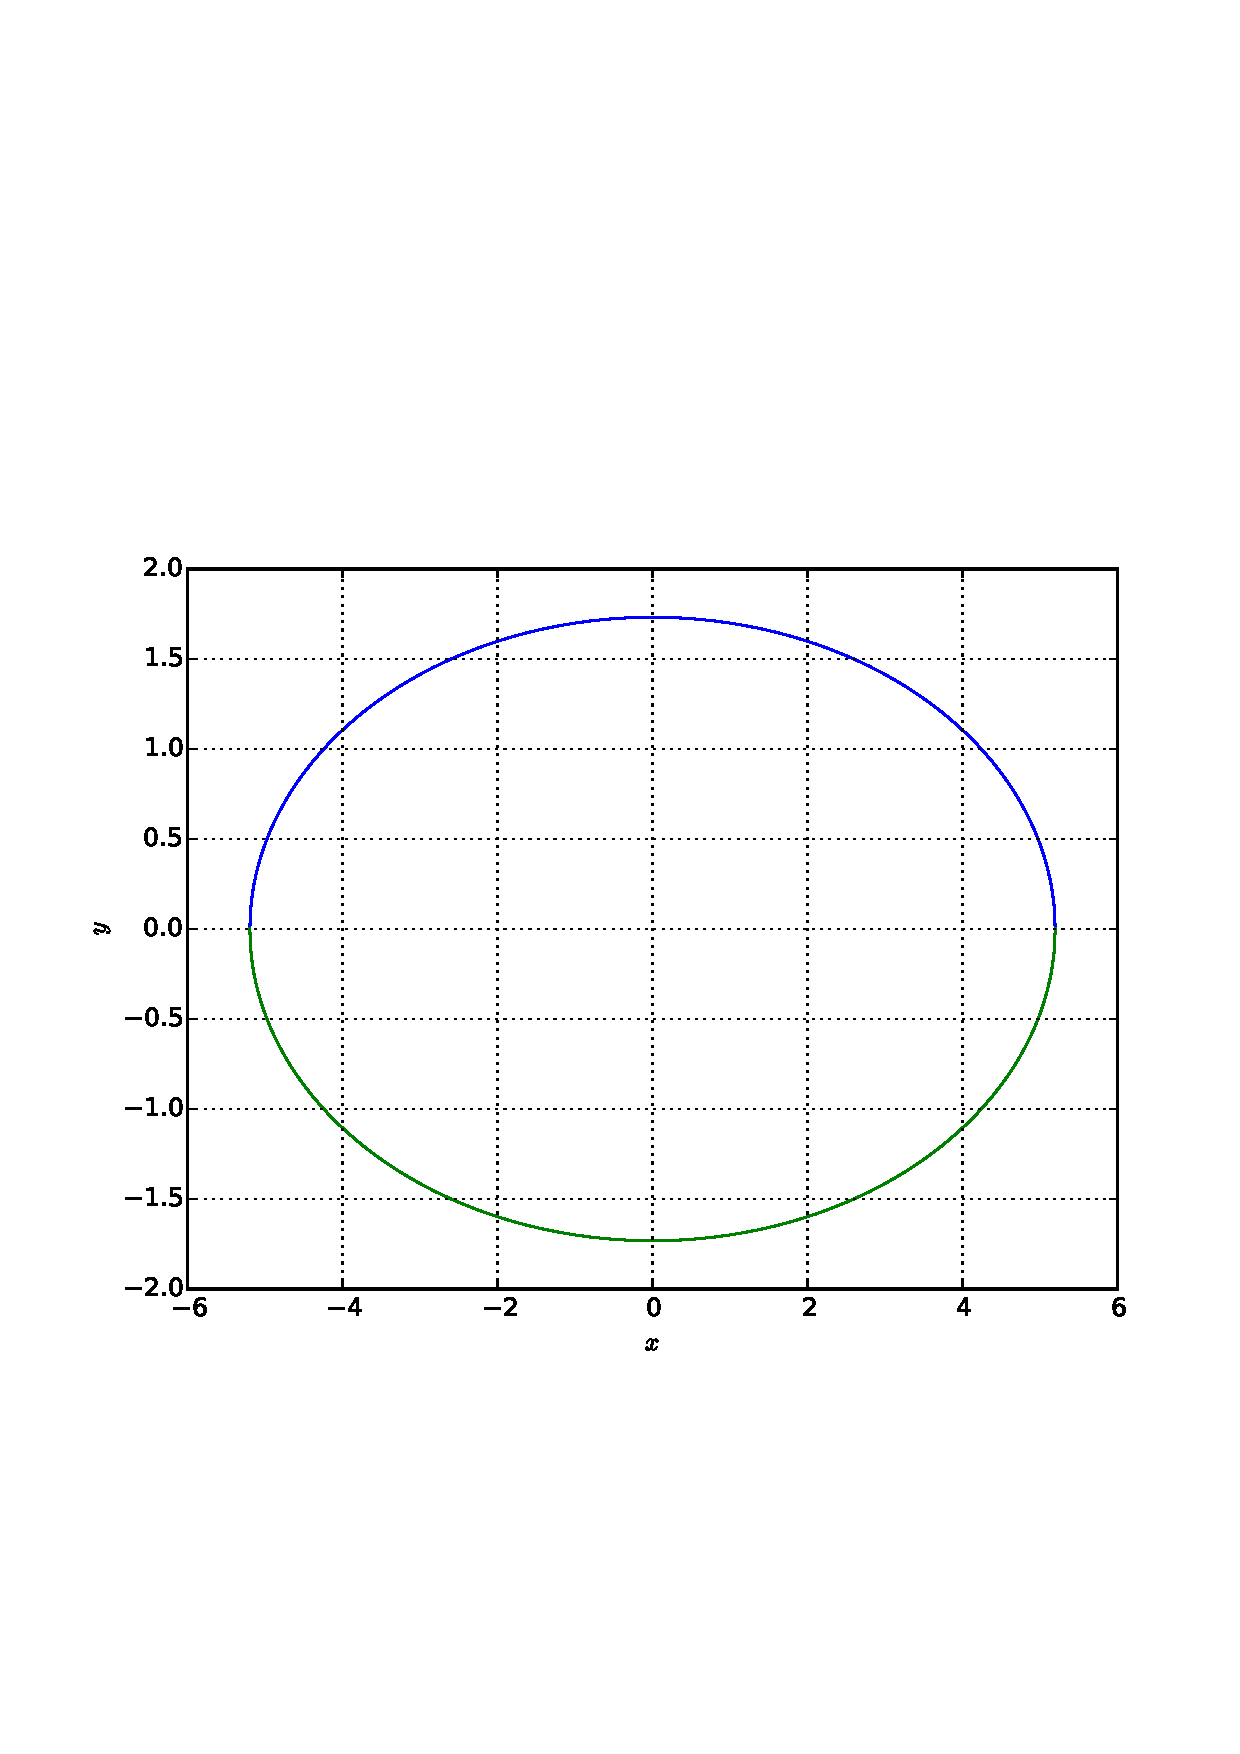
\includegraphics[width=\columnwidth]{./figs/ee16b1013}
\caption{Graph of ellipse $\displaystyle\frac{x^2}{27} +  \frac{y^2}{3} = 1$ }
\label{fig_13}	
\end{figure}
%
\begin{problem}
Find the minimum and maximum values of $4 + \frac{1}{2}\sin^22x - 2\cos^4 x, x \in \mathbf{R}$. 
\end{problem}
\solution 
From the given information,
%
\begin{align}
y &= 4 + \frac{1}{2}\sin^2 2x -2 \cos ^4 x \\
&= 4 + 2\sin^2 x \cos^2 x - 2 \cos ^4 x \\
&= 2 + 2\sin^2 x \cos^2 x + 2 \sin^2 x\brak{1+\cos ^2 x} \\
&= 2 + 4\sin^2 x \cos^2 x + 2 \sin^2 x \\
&= 4 - \cos 2 x - \cos^2 2x\\
& = 4 + \frac{1}{4}-\brak{\cos 2x + \frac{1}{2}} 
\end{align}
%
From the above, it is obvious that the maximum value is $4 \frac{1}{4}$.  From the above, we have
%
\begin{align}
y = 2 + 2\sin^2 2x + 2 \sin^2 x 
\end{align}
%
which has the  minimum value of 2 when $\sin x = 0$.

The following code verifies the above result.
\lstinputlisting{./codes/ee16b1014.py}
\begin{figure}[h]
\centering
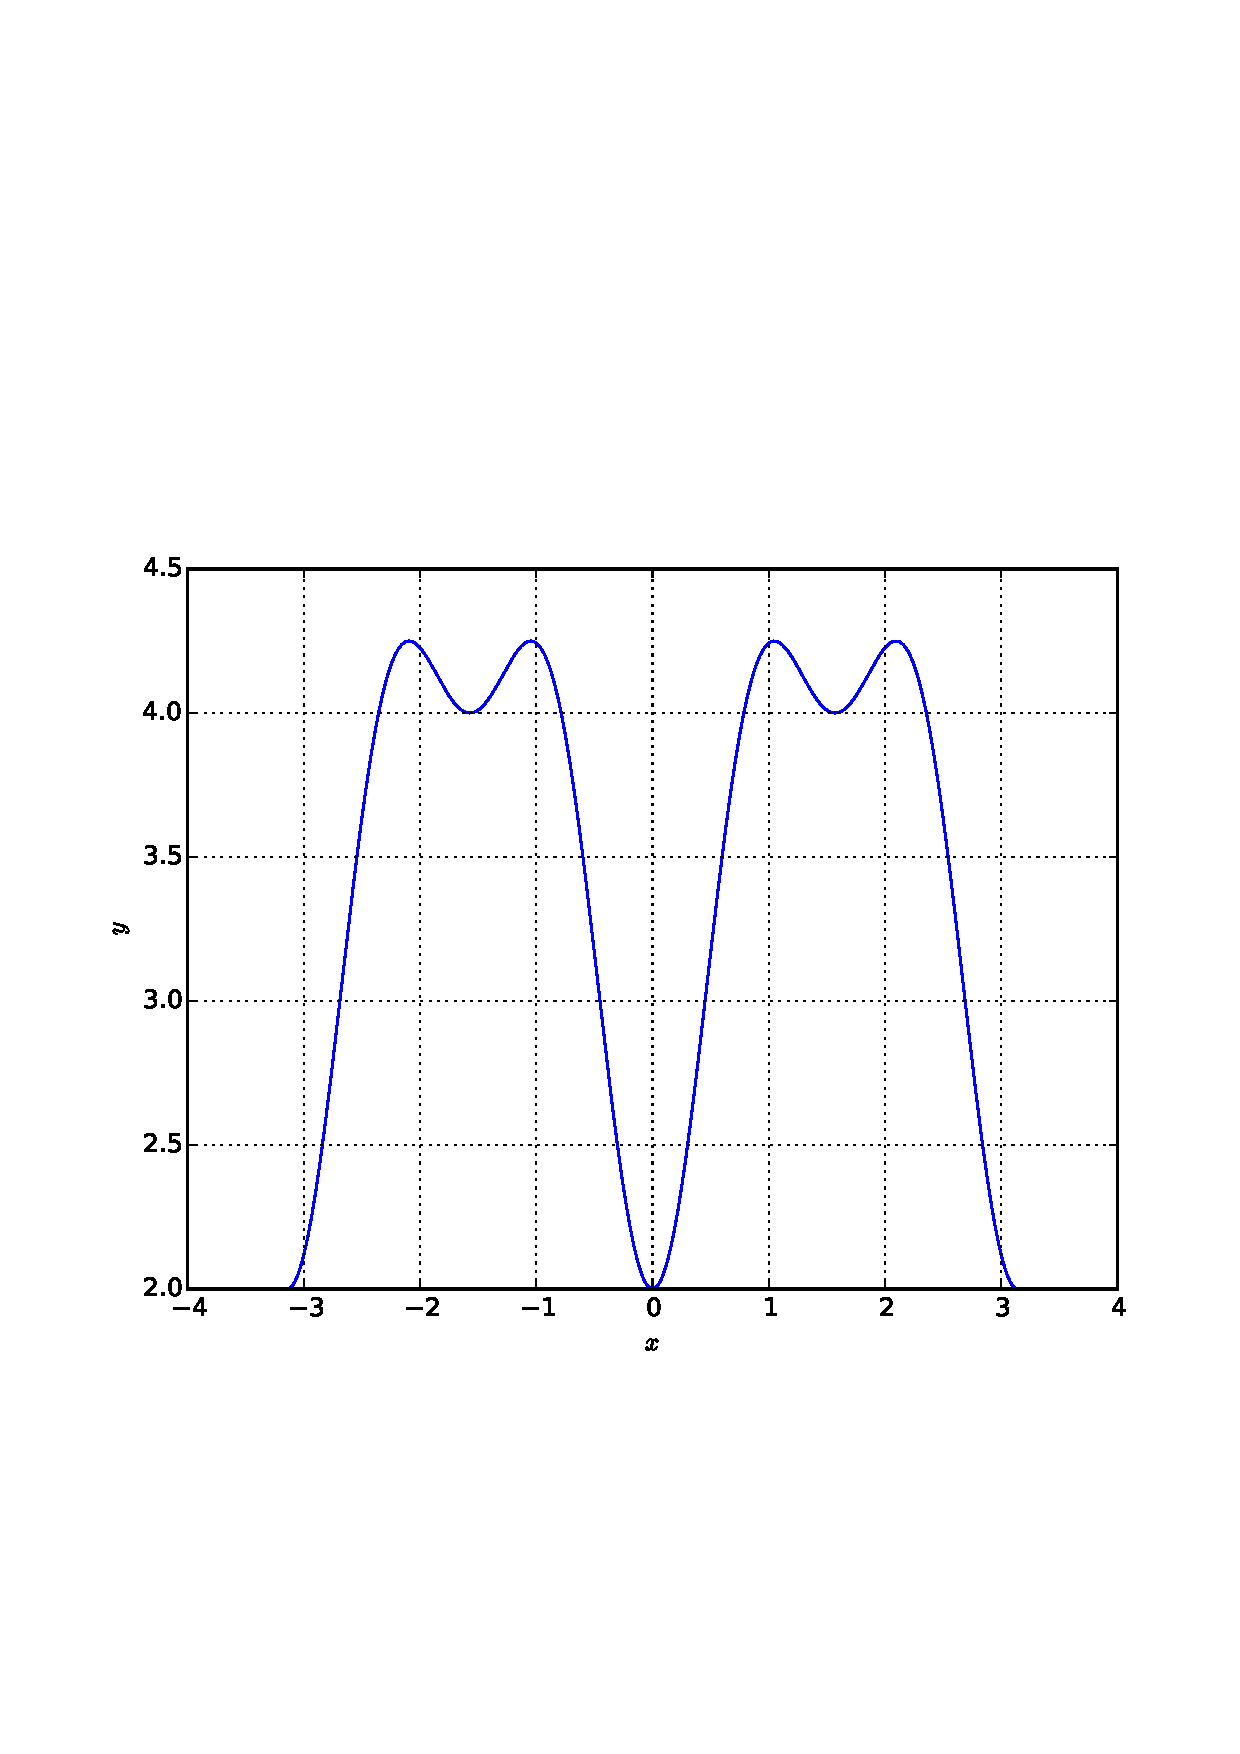
\includegraphics[width=\columnwidth]{./figs/ee16b1014}
\caption{Minimum value is 2 and maximum is $4\frac{1}{4}$}.
\label{fig_14}	
\end{figure}
%
\begin{problem}
Find the solution of the equation $\sqrt{2x+1}- \sqrt{2x-1} = 1, x \geq \frac{1}{2}$.
\end{problem}
\solution
Since 
%
\begin{align}
\brak{\sqrt{2x+1}-\sqrt{2x-1}}\brak{\sqrt{2x+1}+\sqrt{2x-1}} &= 2, \nonumber \\
\brak{\sqrt{2x+1}+\sqrt{2x-1}} &= 2 \nonumber \\
\Rightarrow \sqrt{2x+1} = \frac{3}{2} \Rightarrow x = \frac{5}{8}
\end{align}
%






The graphical solution is available in Fig. \ref{fig_15}
\lstinputlisting{./codes/ee16b1015.py}
\begin{figure}[h]
\centering
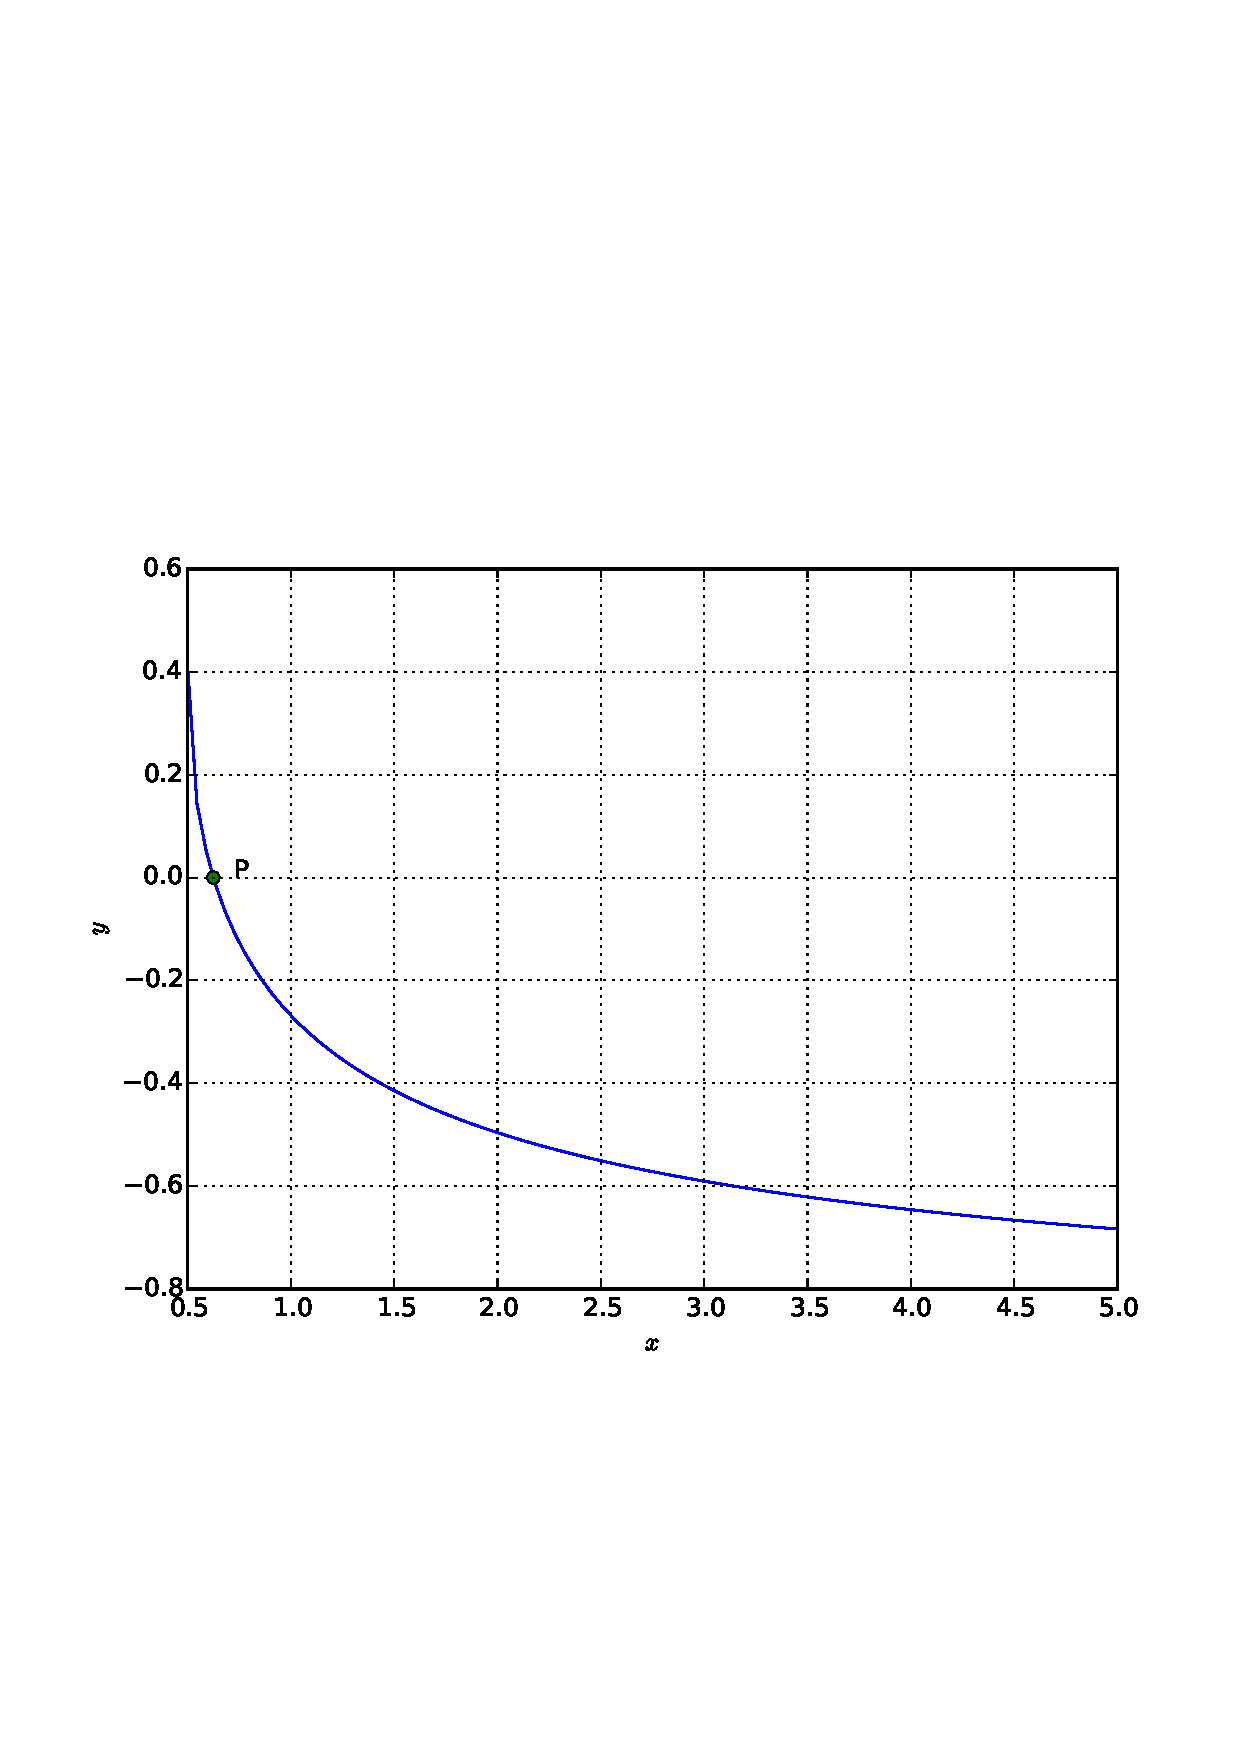
\includegraphics[width=\columnwidth]{./figs/ee16b1015}
\caption{ $\sqrt{2x+1}- \sqrt{2x-1} - 1$ intersects the $x$-axis at $x = \frac{5}{8}$}
\label{fig_15}	
\end{figure}
\begin{problem}
Let $z = 1 + a \i, a > 0$  be a complex number such that $z^3$ is a real number. Find $\sum_{k = 0}^{11}z^k$.
\end{problem}
\solution
\begin{align}
z^3&=(1+ai)^3 \\
&=(1-3a^2)+(3a-a^3)
\end{align}
 Since $z^3$ is a real number,
\begin{align}
\Im(z)=0 \\
\Rightarrow 3a-a^3&=0
\end{align}
%
Since $a > 0$, the desired solution is $a = \sqrt{3}$.
Hence $z=1+\sqrt{3}\i= 2e^{\frac{\i\pi}{3}}$ and
\begin{align}
  \displaystyle\sum\limits_{k=0}^{11} z^k &= \displaystyle\frac{(z^{12}-1)}{z-1}   \\
&=\frac{2^{12}e^{\frac{\i12\pi}{3}}}{1+\sqrt{3}\i-1}\\ 
&=\frac{2^{12}}{\sqrt{3}\i}
\end{align}


The following code provides numerical solutions.  $a$ can be found through Fig. \ref{fig_16}.
\lstinputlisting{./codes/ee16b1016.py}
\begin{figure}[h]
\centering
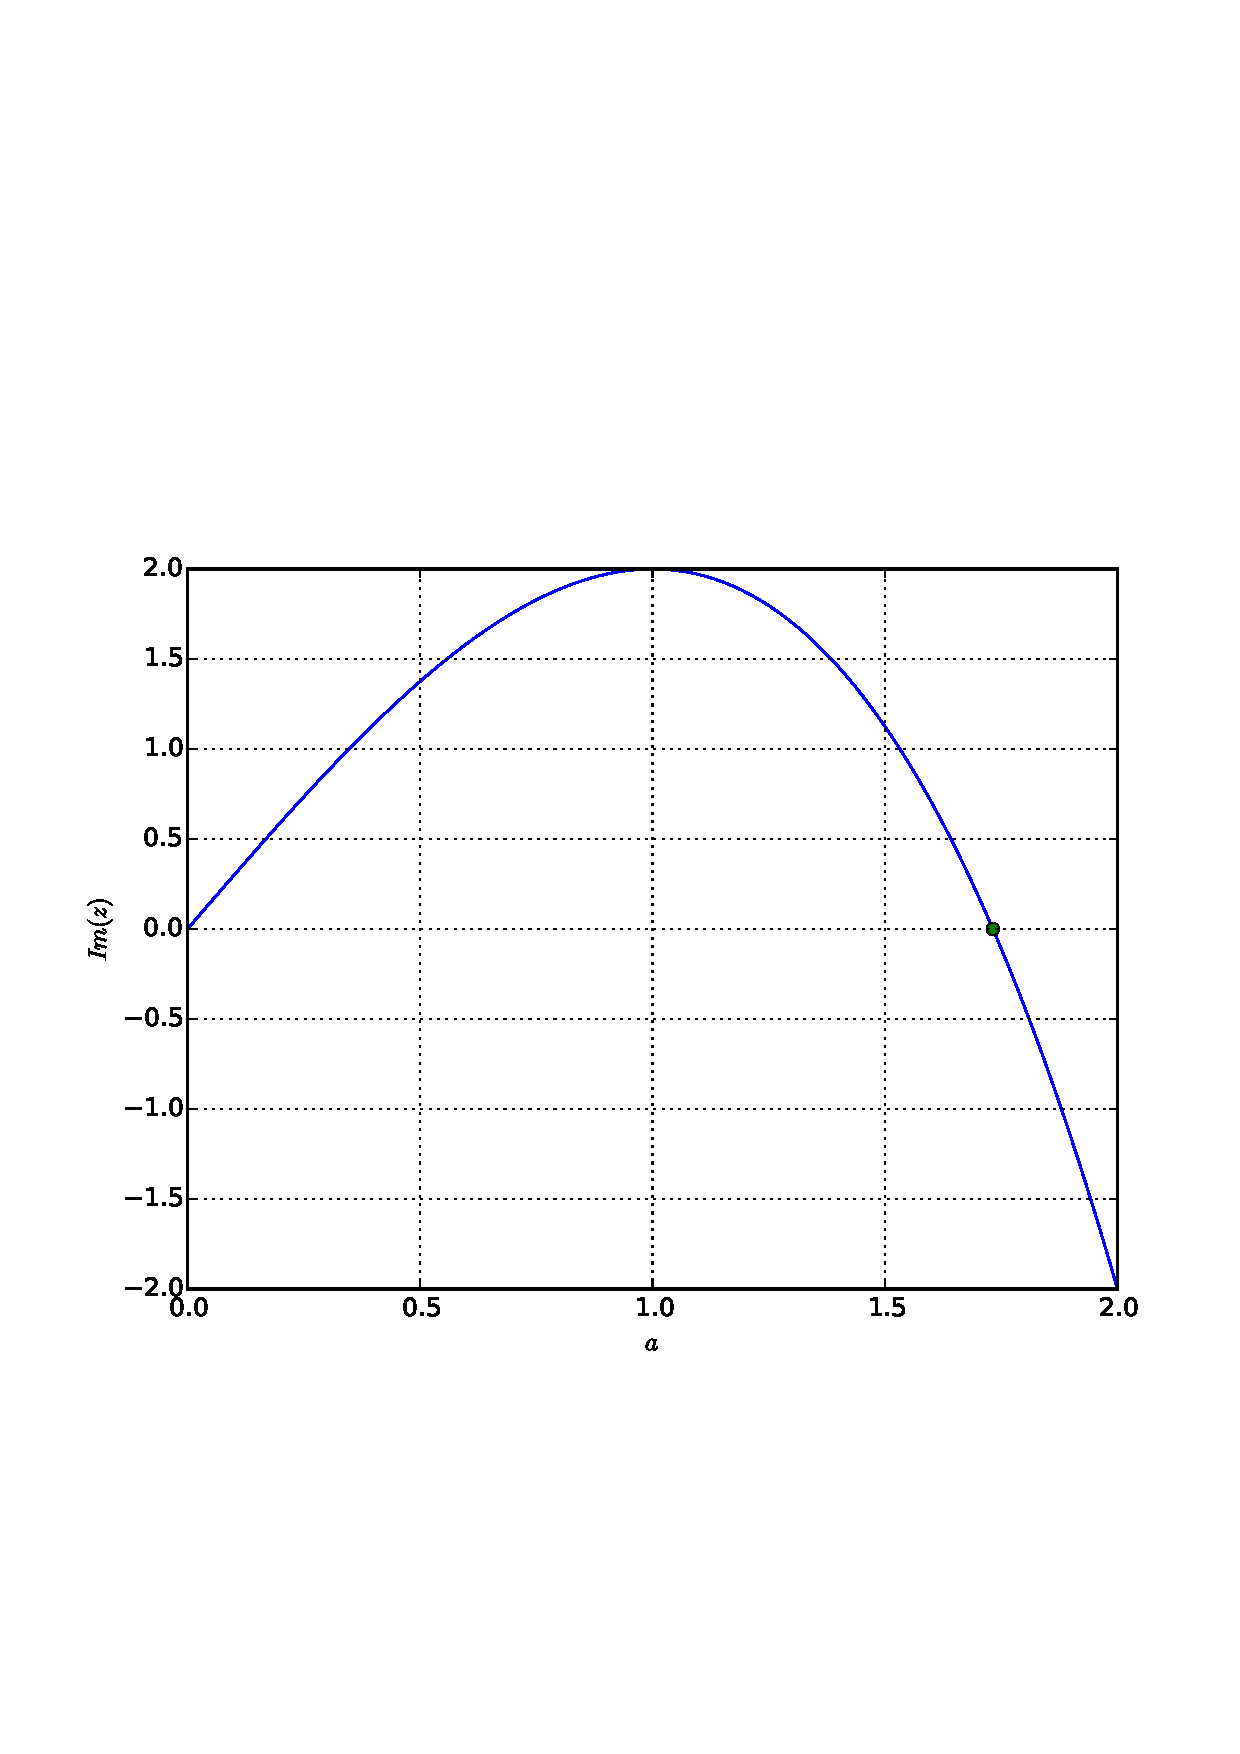
\includegraphics[width=\columnwidth]{./figs/ee16b1016}
\caption{ For positive values, $\Im(z)$ intersects the $x$-axis at $a = \sqrt{3}$.}
\label{fig_16}	
\end{figure}
%
\begin{problem}
$A = 
\begin{pmatrix}
-4 & -1 \\
3 & 1
\end{pmatrix}
$.
Find the determinant of $A^{2016}-2A^{2015}-A^{2014}$.
\end{problem}
%
\solution
%
The given matrix expression can be simplified as
%
\begin{align}
A^{2016}-2A^{2015}-A^{2014} = A^{2014}\brak{A^2-2A-I} 
\end{align}
%
The characteristic equation for the matrix $A$ is obtained as
%
\begin{align}
det(A-\lambda I) &= 0
\\
\Rightarrow \brak{\lambda +4}\brak{\lambda -1} +3 &= 0
\\
\Rightarrow \lambda^2 +3 \lambda -1 = 0
\end{align}
%
From the Cayley-Hamilton theorem,
%
\begin{equation}
A^2+3A-I = 0 \Rightarrow A^2-2A-I = -5A
\end{equation}
%
Since $det(A) = -1, det(-5A) = -25$.

The following code provides the numerical solution to the given problem.
\lstinputlisting{./codes/ee16b1017.py}
%
\begin{problem}
Find the solutions of the following equations
\begin{align*}
n^2-3n-108 &= 0 \\
n^2 + 5n -84 &= 0 \\
n^2 + 2n - 80 &=0 \\
n^2+n-110 &= 0
\end{align*}
Which of these satisfy $\frac{\nCr{n+2}{6}}{\nPr{n-2}{2}} = 11$?
\end{problem}		
%
%
\solution
%
From the following code, the solution to each of the above equations are $n = 12,7, 8$ and $10$ respectively. The given condition can be expressed as
%
\begin{align}
\frac{\nCr{n+2}{6}}{\nPr{n-2}{2}} &= 11 \\
\Rightarrow \frac{\brak{n+2}!}{\brak{n-4}!6!}\frac{\brak{n-4}!}{\brak{n-2}!} &= 11 \\
\Rightarrow \frac{n\brak{n-1}\brak{n+1}\brak{n+2}}{6!} &=11
\end{align}
%

From the above equation, it is obvious that the correct solution is 9.  So none of the solutions
of the given equations satisfy the given condition.  This is verified numerically through the following code.
\lstinputlisting{./codes/ee16b1018.py}
%

\begin{problem}
Sketch 
\begin{equation*}
f(x) = 
\begin{cases}
\frac{2x^2}{a} & 0 \leq x < 1\\
a & 1 \leq x < \sqrt{2} \\
\frac{2b^2 - 4b}{x^3} & \sqrt{2} \leq x < \infty
\end{cases}
\end{equation*}
for $\brak{a,b}$ equal to 
\begin{enumerate}
\item $\brak{\sqrt{2}, 1 - \sqrt{3}}$
\item $\brak{-\sqrt{2}, 1 + \sqrt{3}}$
\item $\brak{\sqrt{2},-1+\sqrt{3}}$
\item $\brak{-\sqrt{2}, 1 - \sqrt{3}}$
\end{enumerate}
In which case is  $f(x)$ continuous?
\end{problem}
%
\solution The following python code generates the following figures
\lstinputlisting{./codes/ee16b1019.py}

\renewcommand{\thefigure}{\theproblem.\arabic{figure}}
\begin{figure}[h]
\centering
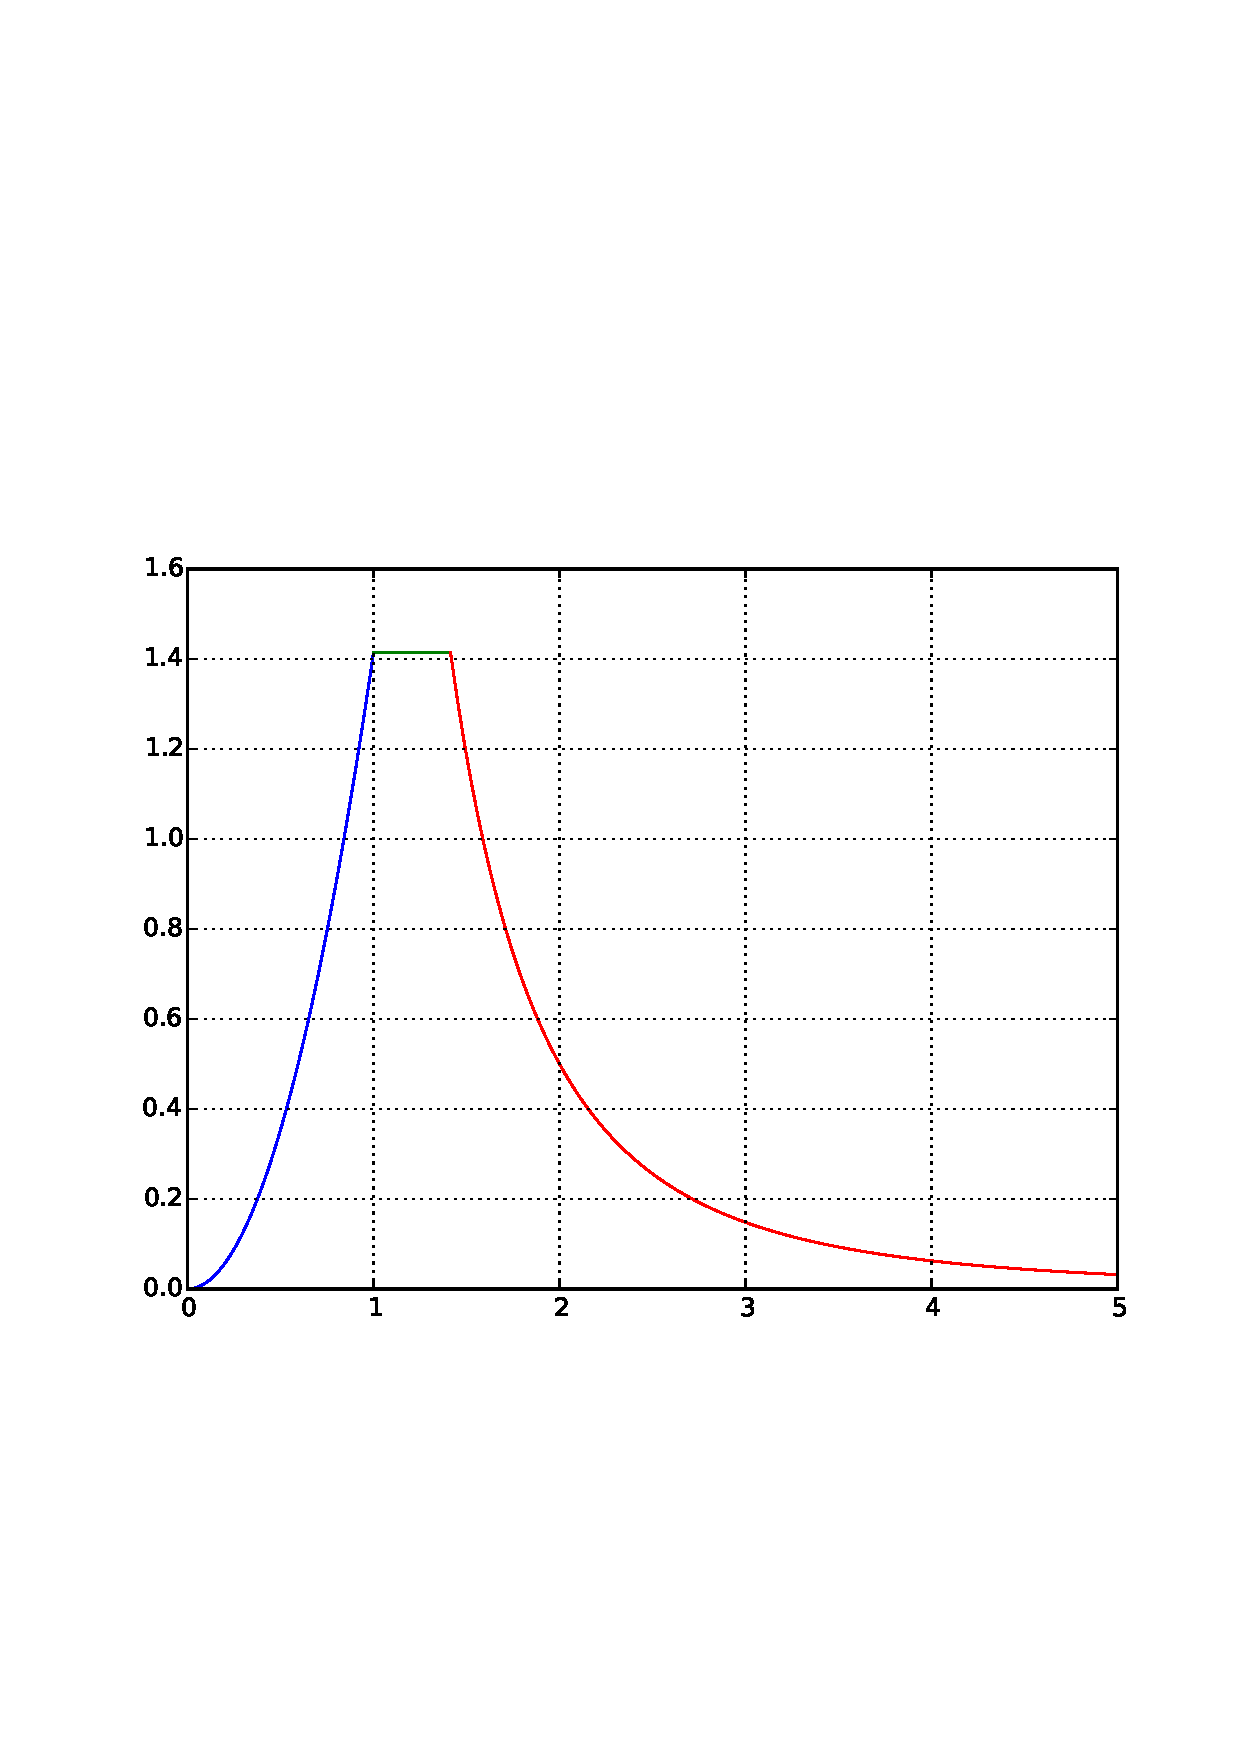
\includegraphics[width=\columnwidth]{./figs/ee16b1019a}
\caption{ Continuous for $\brak{\sqrt{2}, 1 - \sqrt{3}}$}
%\label{fig_16}	
\end{figure}
%
\begin{figure}[h]
\centering
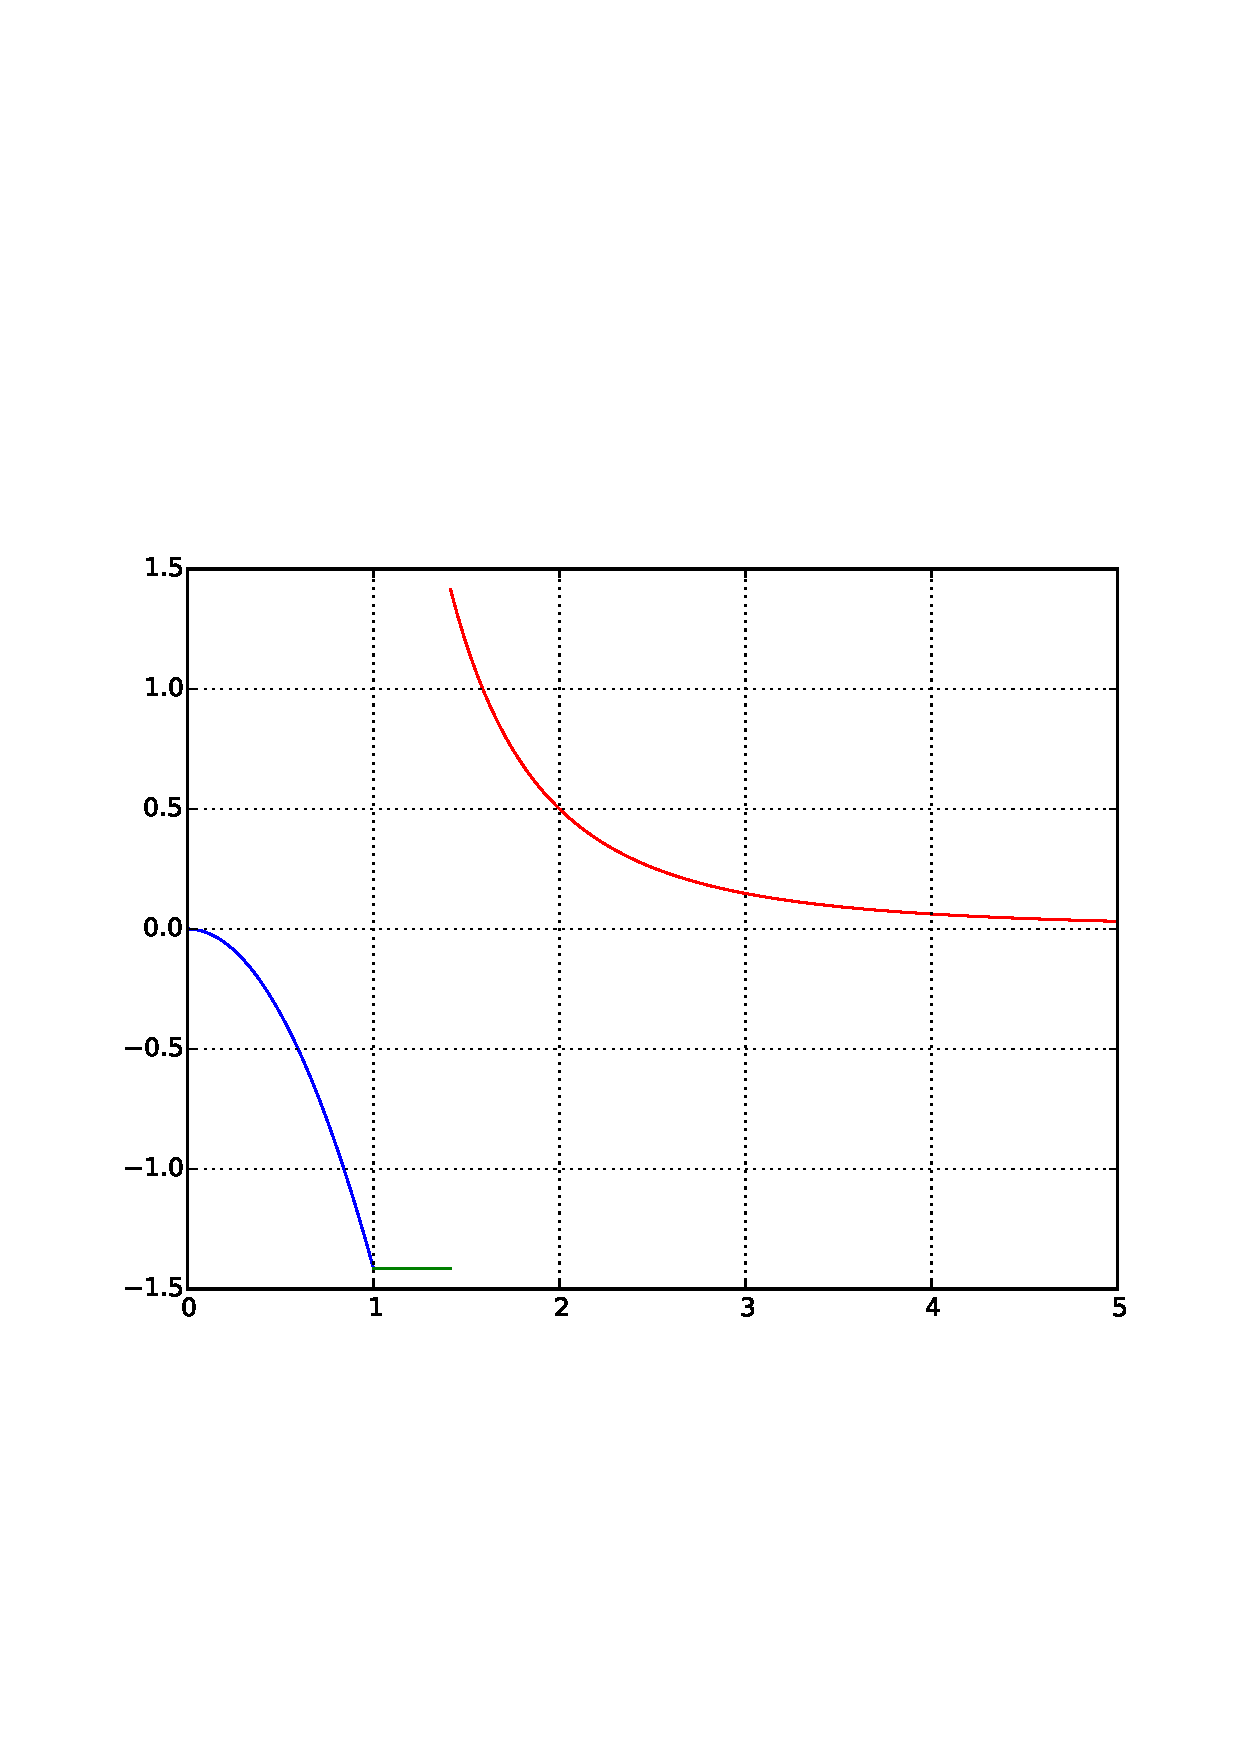
\includegraphics[width=\columnwidth]{./figs/ee16b1019b}
\caption{ Discontinuous for $\brak{-\sqrt{2}, 1 + \sqrt{3}}$}
%\label{fig_16}	
\end{figure}
%
\begin{figure}[h]
\centering
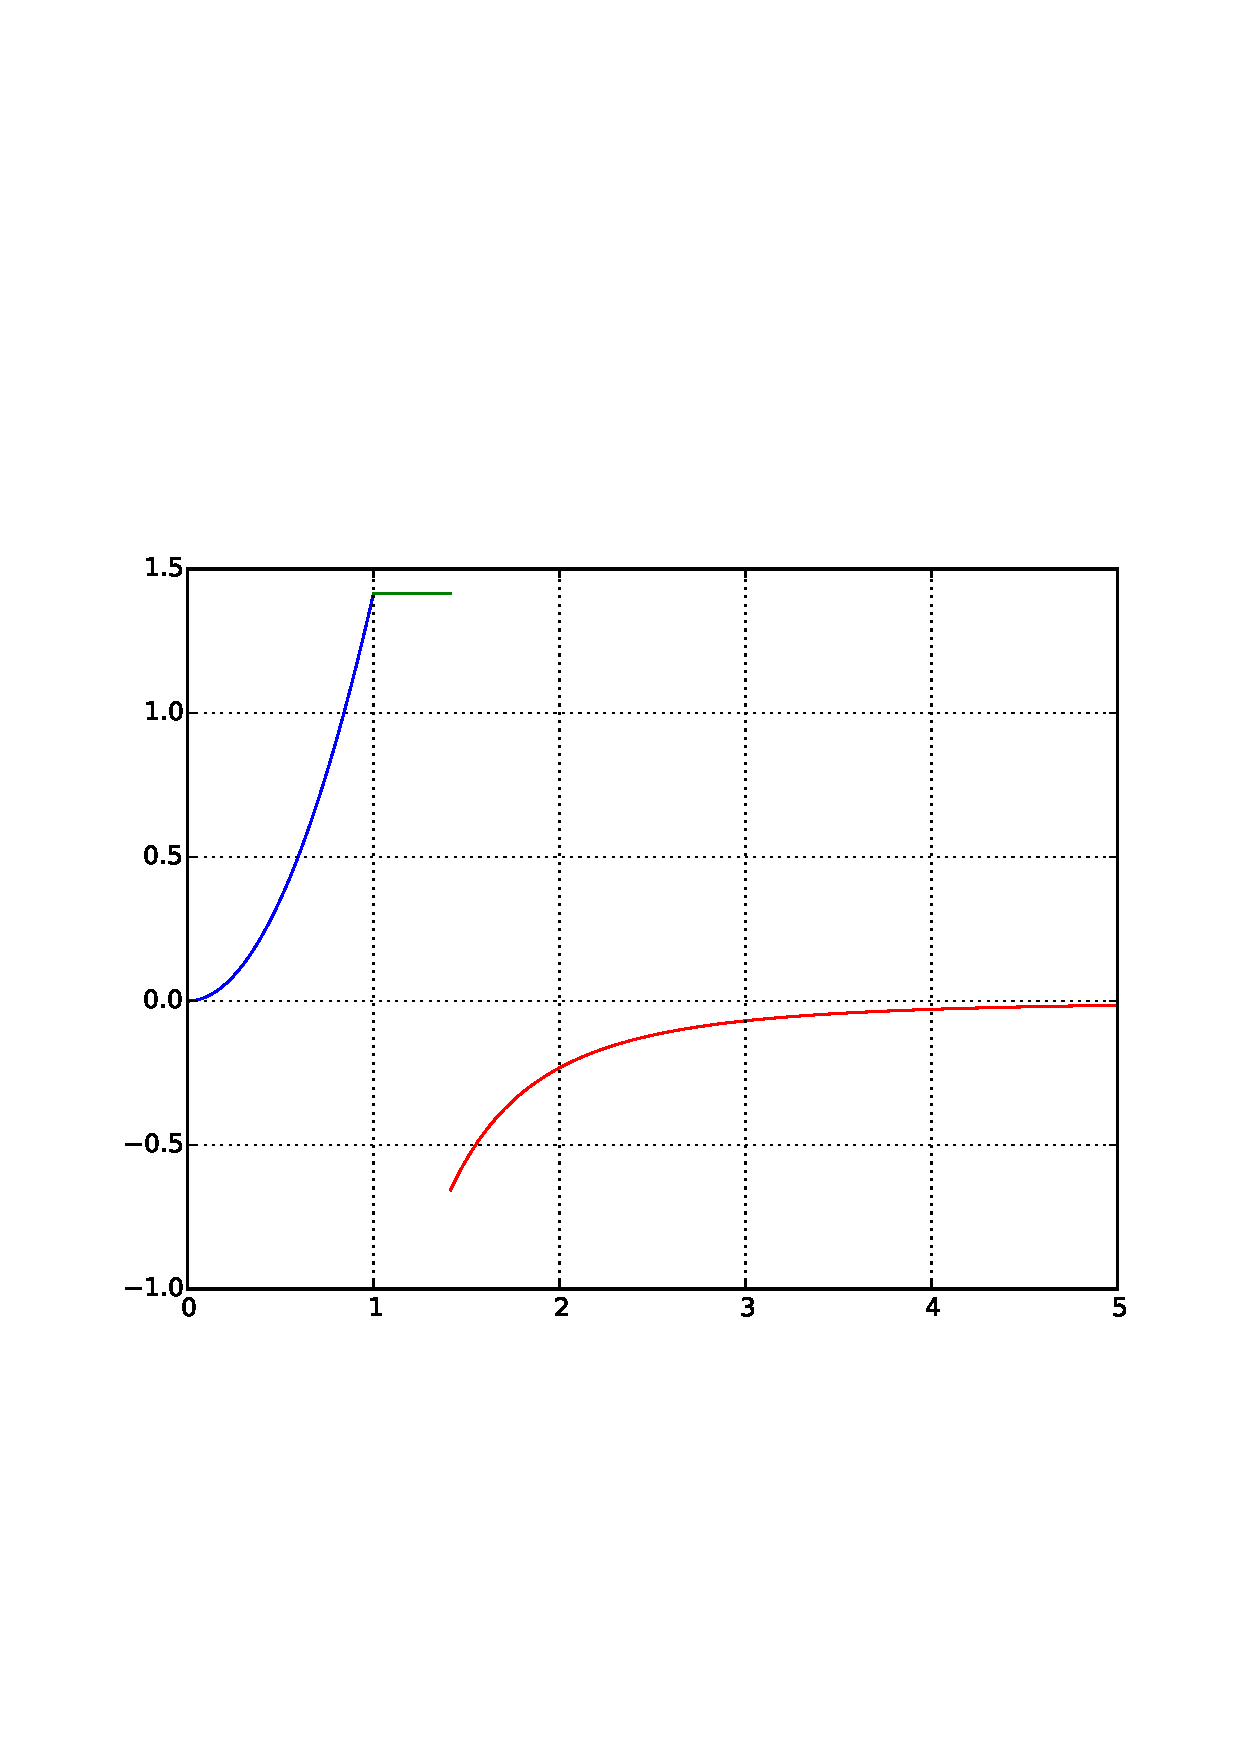
\includegraphics[width=\columnwidth]{./figs/ee16b1019c}
\caption{ Continuous for $\brak{\sqrt{2}, 1 + \sqrt{3}}$}
%\label{fig_16}	
\end{figure}
%
\begin{figure}[h]
\centering
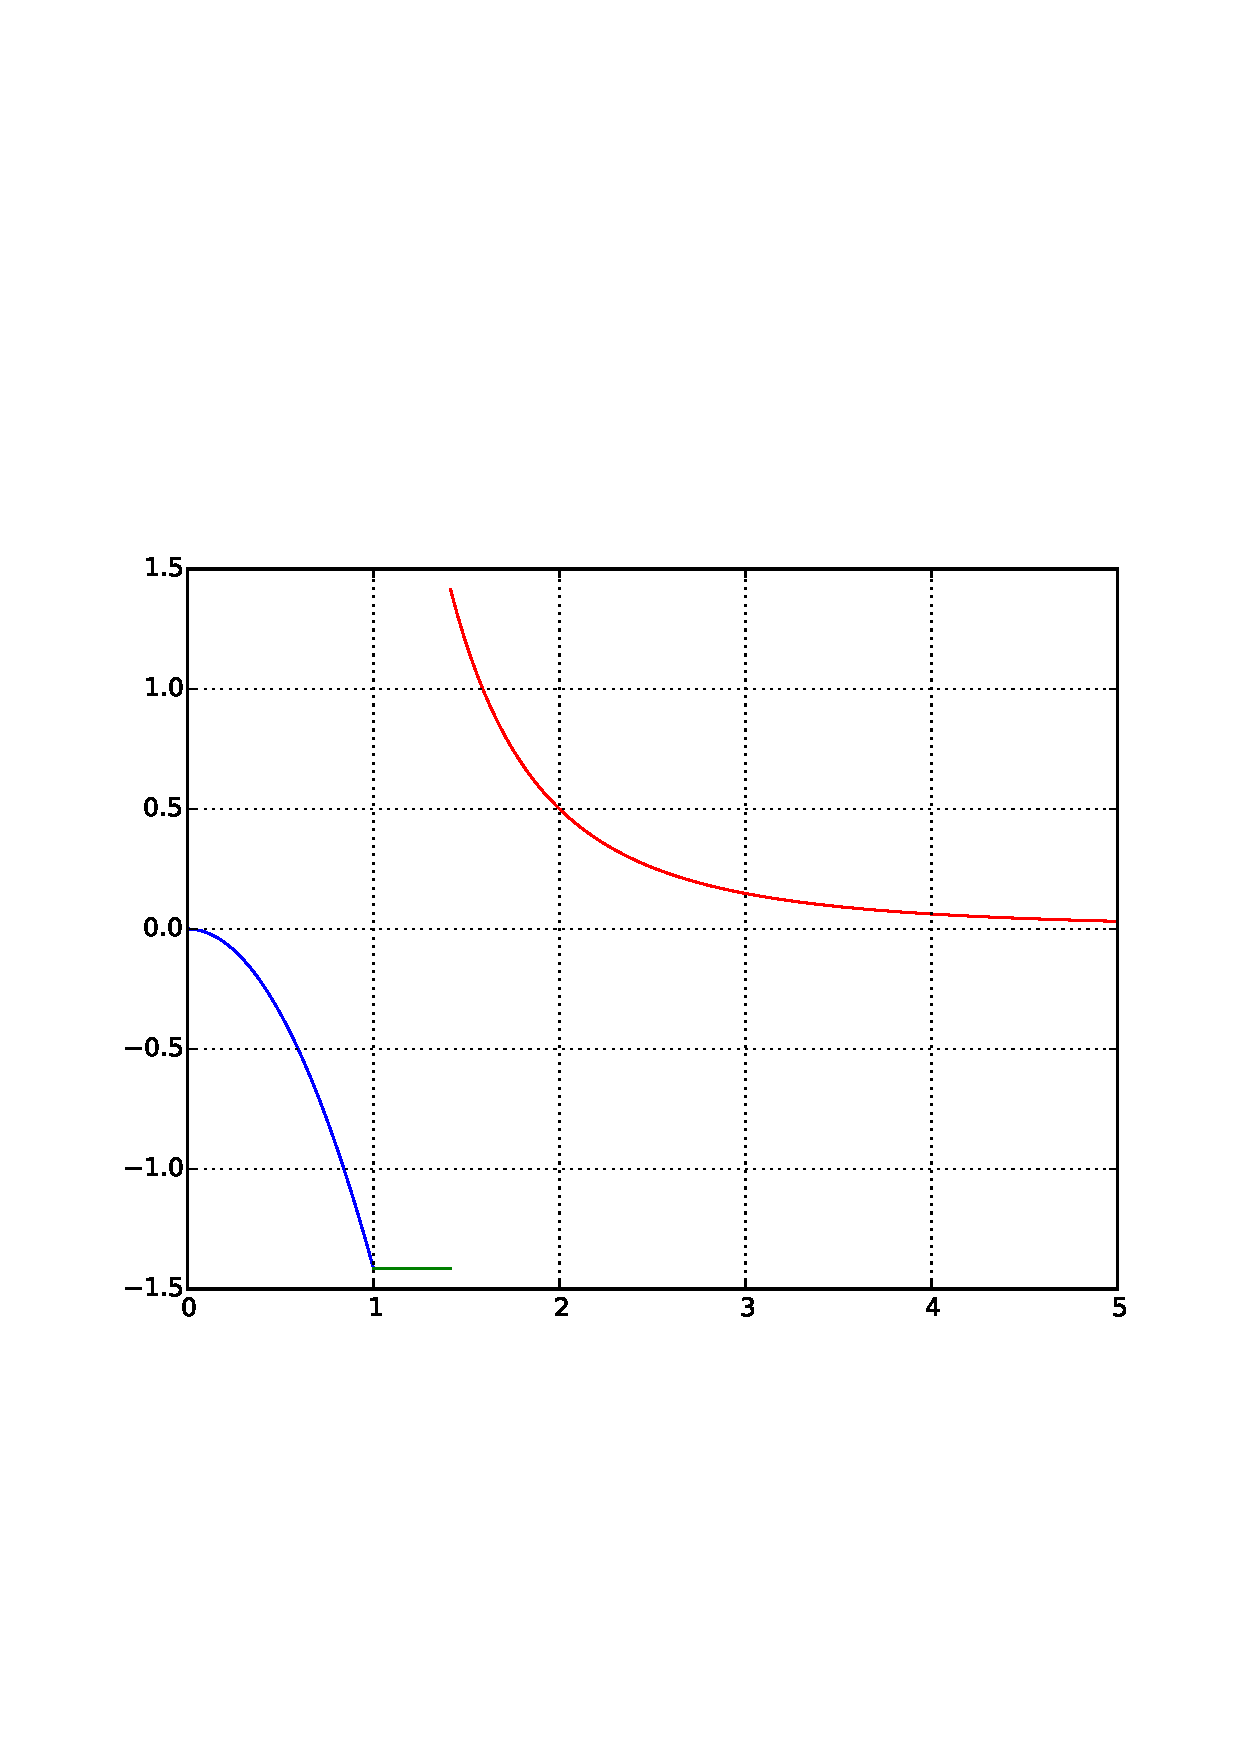
\includegraphics[width=\columnwidth]{./figs/ee16b1019d}
\caption{ Discontinuous for $\brak{-\sqrt{2}, 1 - \sqrt{3}}$}
%\label{fig_16}	
\end{figure}
%
\renewcommand{\thefigure}{\theproblem}
\begin{problem}
Sketch $f(x) = \sin^4x + \cos^4x$. Find the intervals within $\brak{0,\pi}$ when it is increasing.
\end{problem}
\solution The following code plots the graph in Fig. \ref{fig_20} outlining the intervals when the function is increasing.
\lstinputlisting{./codes/ee16b1020.py}
%
\begin{figure}[h]
\centering
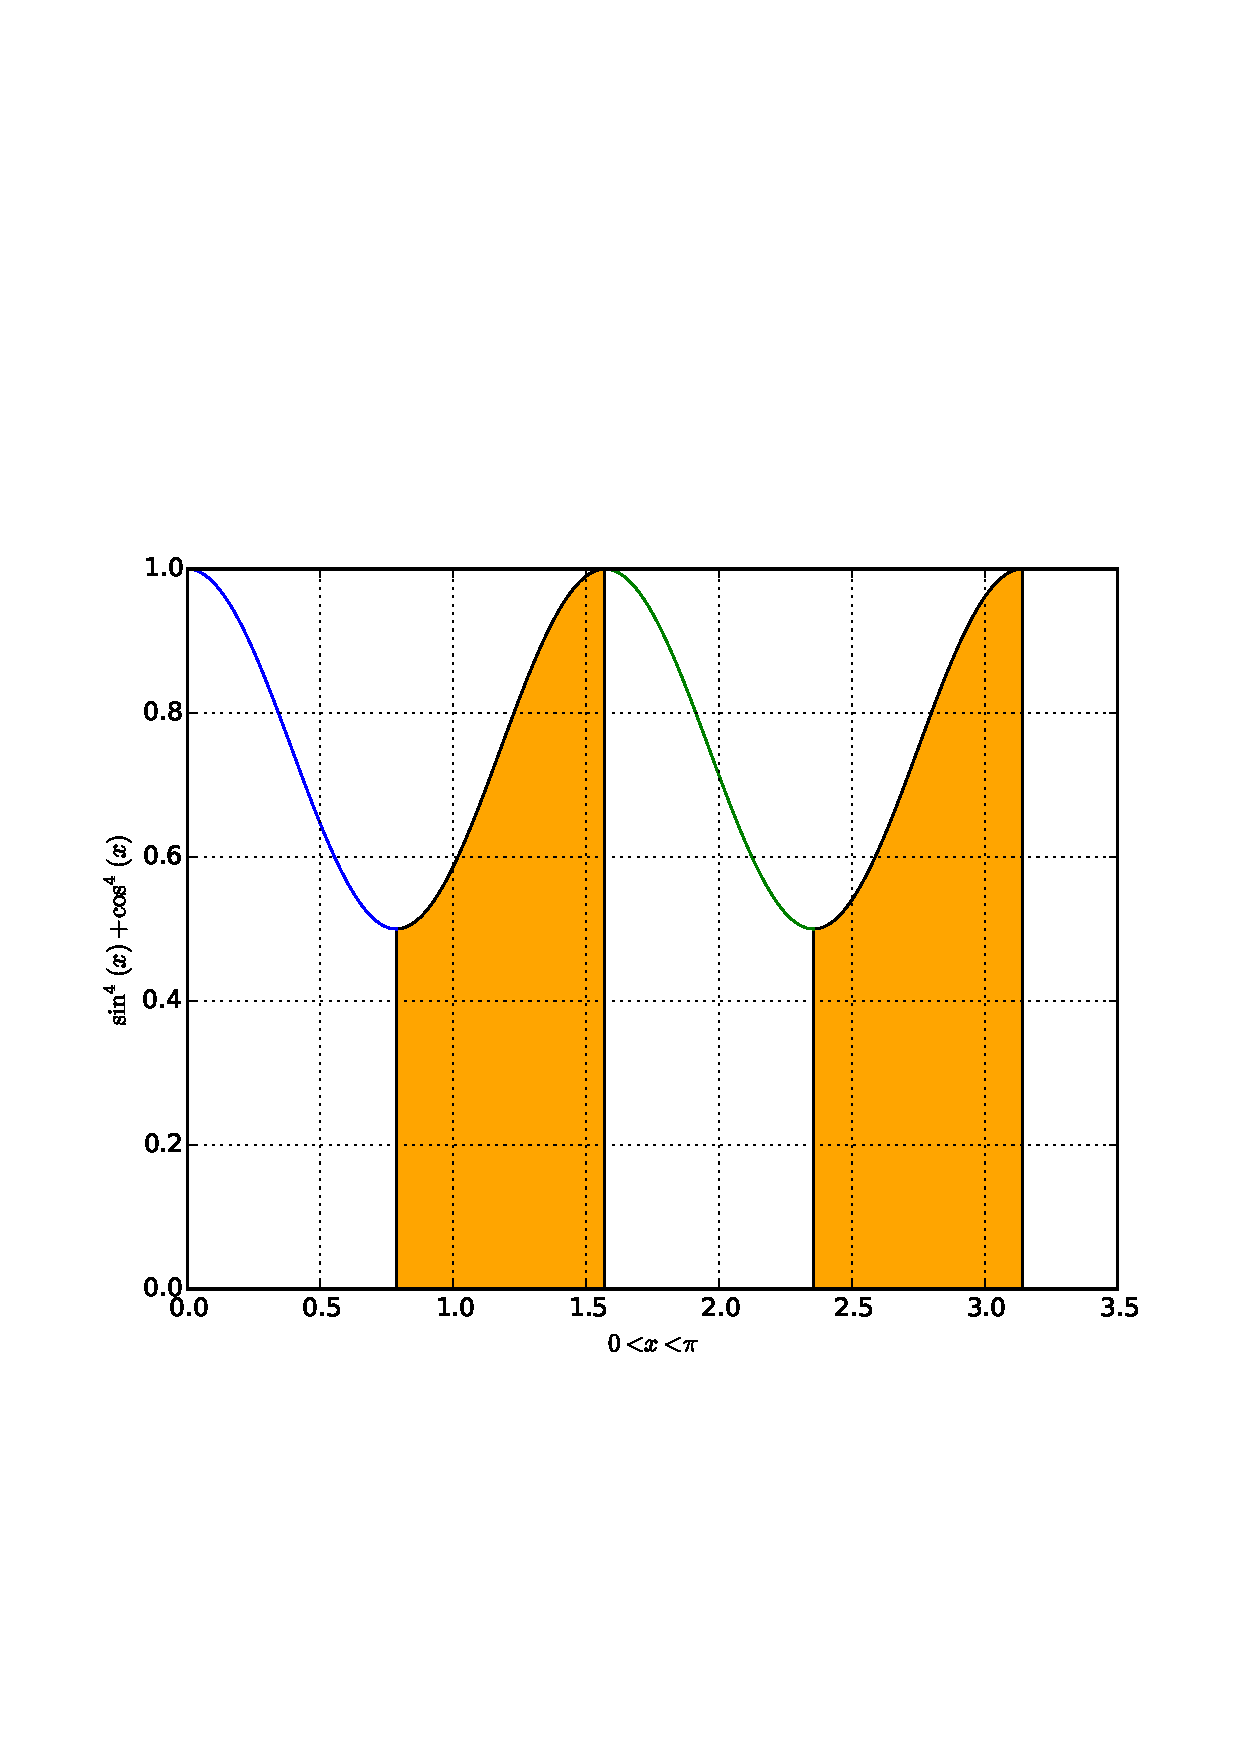
\includegraphics[width=\columnwidth]{./figs/ee16b1020}
\caption{ The green shaded region is where the function is increasing.}
\label{fig_20}	
\end{figure}
%
\begin{problem}
The reflected line is given by $y+2x=1$. The surface is given by $7x-y+1=0$. Which of the following is the incident line?
\begin{enumerate}
\item $41x - 38y +38 = 0$
\item $41x +25y - 25 = 0$
\item $41x + 38y-38=0$
\item $41x-25y+25=0$
\end{enumerate}
\end{problem}
\solution
The point at which the reflected line touches the surface is the solution of the equation
%
\begin{equation}
A = 
\begin{pmatrix}
2 &1 \\
 7 & -1
 \end{pmatrix}
  \begin{pmatrix}
x \\
  y
 \end{pmatrix}
=
 \begin{pmatrix}
1 \\
  -1
 \end{pmatrix}
\end{equation}
%  

%
\begin{equation}
\end{equation}
%
yielding the point $\brak{0,1}$.
Angle   between   the   given   line   is   given   
\begin{equation}
\theta =\tan ^{ -1 }{ \frac { (m_1-m_2) }{ (1+m_1*m_2) }  } 
\end{equation} 
 where   $m_1, m_2$   are   slopes   of   surface   and   reflected   line   respectively.
\begin{equation}\theta =\tan ^{ -1 }{ \frac { (7-(-2)) }{ (1+7*(-2))) }  } 
 \end{equation} 
 \begin{equation}
 \theta =\tan ^{ -1 }{ \frac { -9 }{ 13 }  } 
  \end{equation}  
  The     slope     of     the     incident          line     can     be     found     by     reversing     the     direction     of     the     angle     along     the     surface. Letting the angle that the incident line makes along the $x$-axis to be $\phi$, 
  \begin{equation}
   \phi =\tan ^{ -1 }{ \frac { (m_1-\tan\theta ) }{ (1+m_1*\tan\theta ) }  } 
    \end{equation}
    \begin{equation}
        m=\frac { (7-\frac { 9 }{ 13 } ) }{ (1+7*\frac { 9 }{ 13 } ) } 
        \end{equation}
         \begin{equation}
         m=\frac { (91-9) }{ (63+13) }  \end{equation}
          \begin{equation} 
          m=\frac{41}{38 }
          \end{equation}
           Since     m     is     the     slope     and     1     is     the     intercept     and     thus     in     slope     form     equation     of     line     is     $y=mx+1$. Thus     the     equation     of     the     incident     line     is                                                                              
\begin{equation}
 38y=41x+38
\end{equation}           



The following code  summarises the solution through the plot in Fig. \ref{fig_21}
\lstinputlisting{./codes/ee16b1021.py}
%
\begin{figure}[h]
\centering
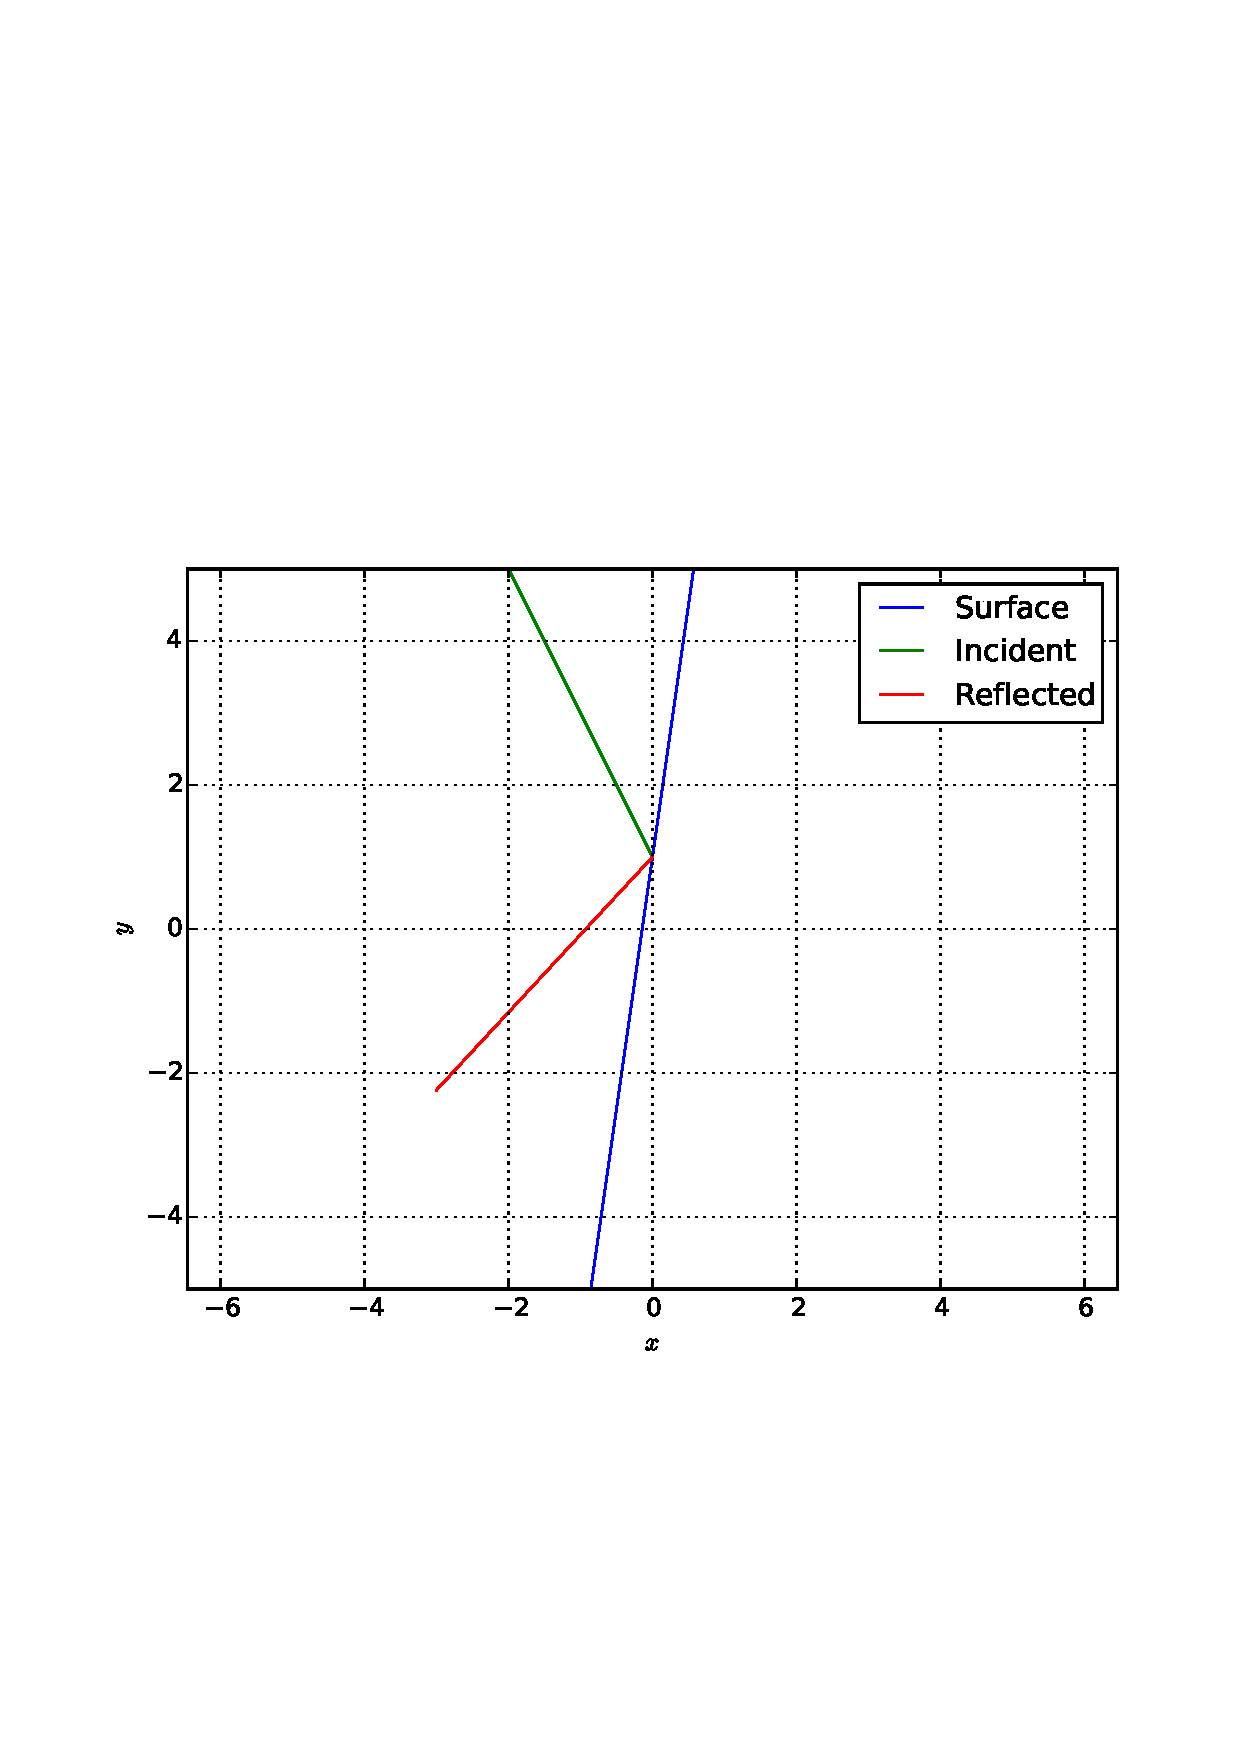
\includegraphics[width=\columnwidth]{./figs/ee16b1021}
\caption{ $41x - 38y +38 = 0$ is the incident line}
\label{fig_21}	
\end{figure}
%
\begin{problem}
The lines $x-y=1$ and $2x+y=3$ intersect at $O$.  A circle with centre at point $O$ passes through the point $\brak{-1,1}$. Sketch the following lines
\begin{enumerate}
\item $4x +y -3 = 0$
\item $x + 4y+3 = 0$
\item $3x - y  - 4 = 0$
\item $x - 3y - 4 = 0$
\end{enumerate}
Which of these is a tangent to the circle? At what point?
\end{problem}
\solution
The lines $x-y=1$ and $2x+y=3$ intersect at the point O, whose coordinates are obtained from the following equation
\begin{equation}
A =
\begin{pmatrix}
1 & -1
\\
 2 & 1
\end{pmatrix}
\begin{pmatrix}
x
\\
y
\end{pmatrix}
\begin{pmatrix}
1 
\\
 3
\end{pmatrix}
\end{equation}
as $\brak{\frac{4}{3},\frac{1}{3}}$.  Since the circle has centre at $O$ and passes trough the point $\brak{1,-1}$, its radius is
%
\begin{equation}
r = \sqrt{\brak{\frac{4}{3}+1}^2+\brak{\frac{1}{3}-1}^2} = \frac{\sqrt{53}}{3}
\end{equation}
%
The equation of the circle is then obtained as
%
\begin{equation}
\brak{x-\frac{4}{3}}^2+\brak{y-\frac{1}{3}}^2=\frac{53}{9}
\end{equation}
% 
%\end{document}    

%
The following python code plots the circle as well as the various lines  in Fig. \ref{fig_22} and shows that no  line is a tangent to the circle.
\lstinputlisting{./codes/ee16b1022.py}
%
\begin{figure}[h]
\centering
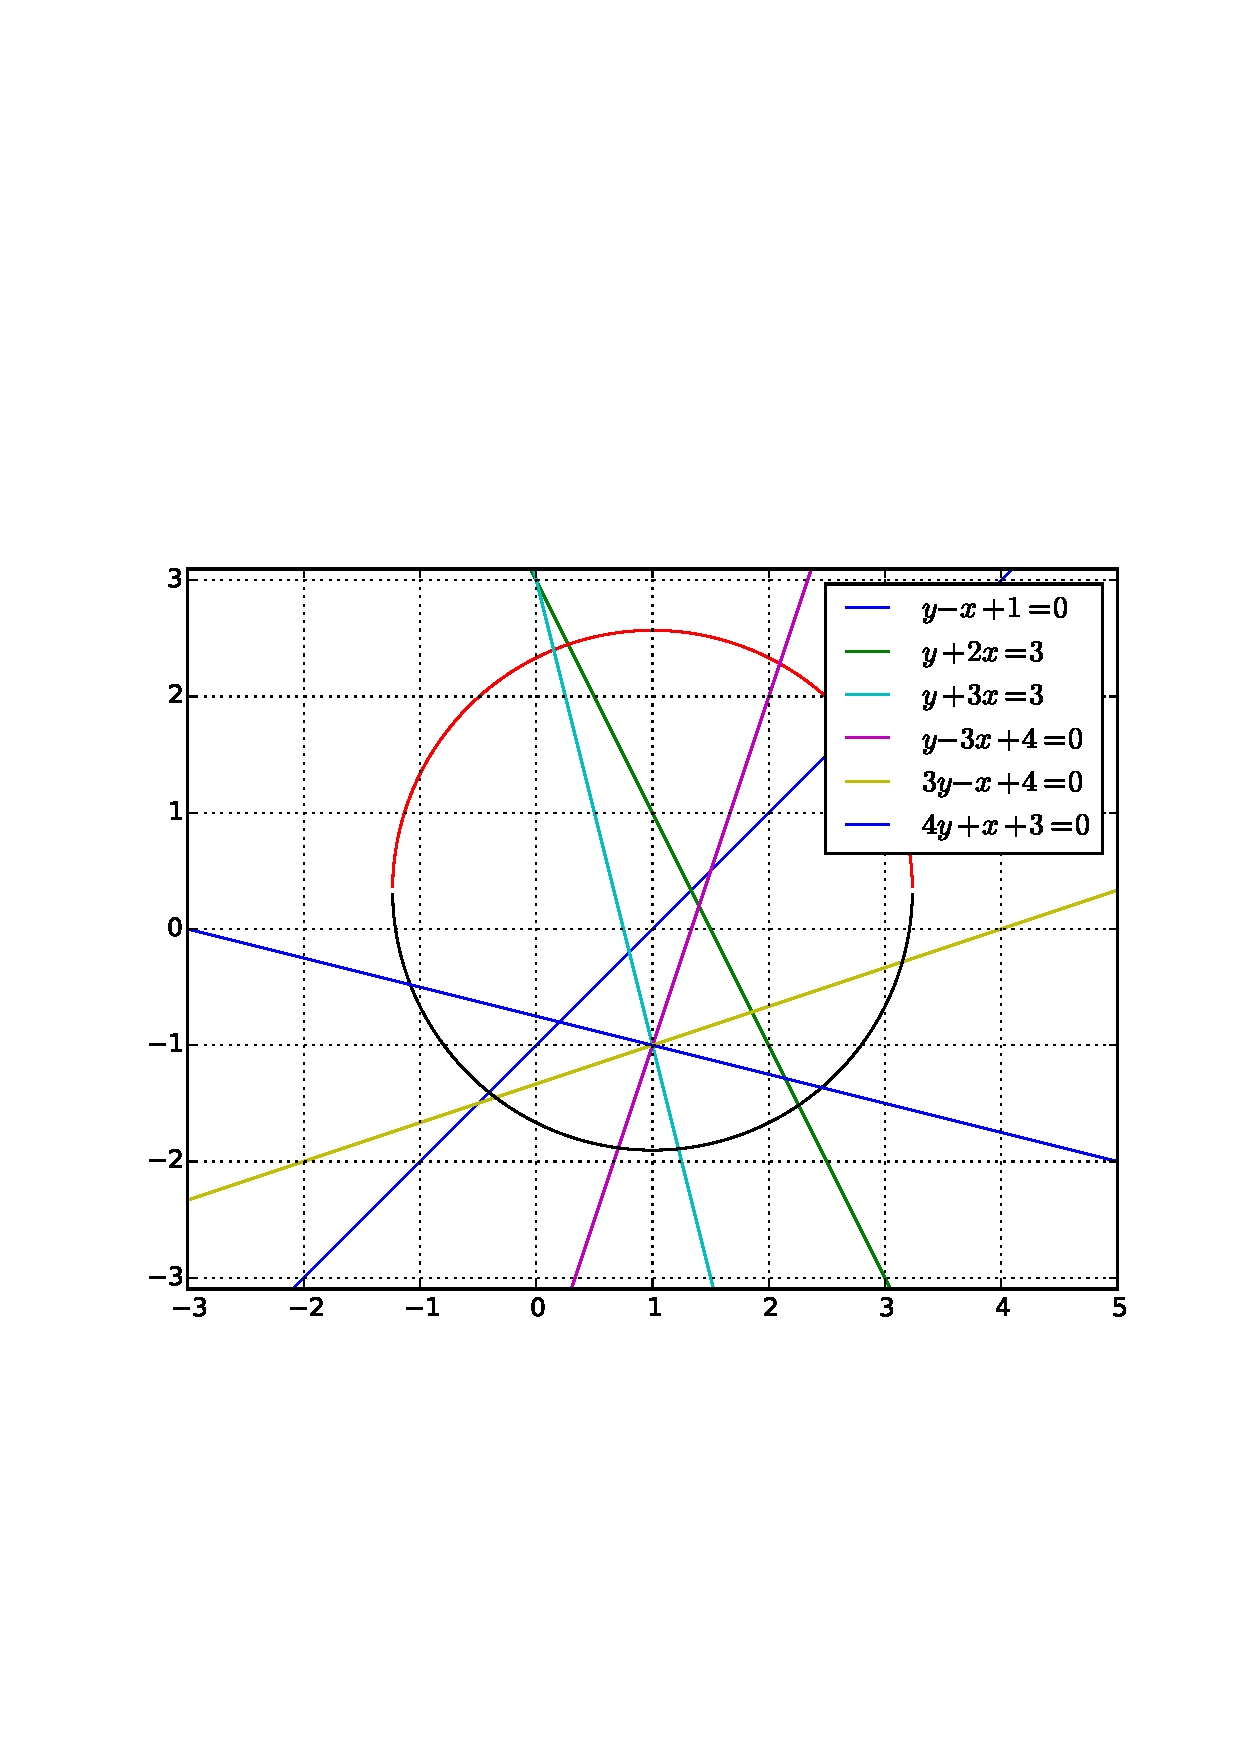
\includegraphics[width=\columnwidth]{./figs/ee16b1022}
\caption{ Since the lines intersect the circle, they are not tangent to it and no point of tangency exists. }
\label{fig_22}	
\end{figure}
%
\begin{problem}
$P$ and $Q$ are distinct points on the parabola $y^2 = 4x$, with parameters $t$ and $t_1$ respectively. The normal at $P$ passes through $Q$.  Find the minimum value of $t_1^2$.
\end{problem}
\solution
Using the parametric form, the points $P$ and $Q$ can be expressed as $\brak{t^2,2t}$ and $\brak{t_1^2,2t_1}$ respectively.  The slope of the normal at $P$ is
%
\begin{equation}
-\frac{dx}{dy} = -\frac{\frac{dx}{dt}}{\frac{dy}{dt}} = - t
\end{equation}
%
The equation of the normal is then obtained as
%
\begin{align}
\brak{y - 2t} &= -t\brak{x -t^2} \\
\Rightarrow 2\brak{t_1-t} &= -t\brak{t_1-t}\brak{t_1+t} \\
\Rightarrow t_1 &= -\brak{t + \frac{2}{t}}
\end{align}
%
Thus,
%
\begin{align}
t_1^2 &= 4 + t^2 + \frac{4}{t^2} \\
&= \brak{t - \frac{2}{t}}^2 + 8  
\end{align}
%
and the minimum value of $t_1^2$ is obtained from the above as 8. For this value,
%
\begin{align}
t - \frac{2}{t} = 0 \Rightarrow t = \pm \sqrt{2}
\end{align}
%

The following code provides a visualisation of the problem.
\lstinputlisting{./codes/ee16b1023.py}
%
\begin{figure}[h]
\centering
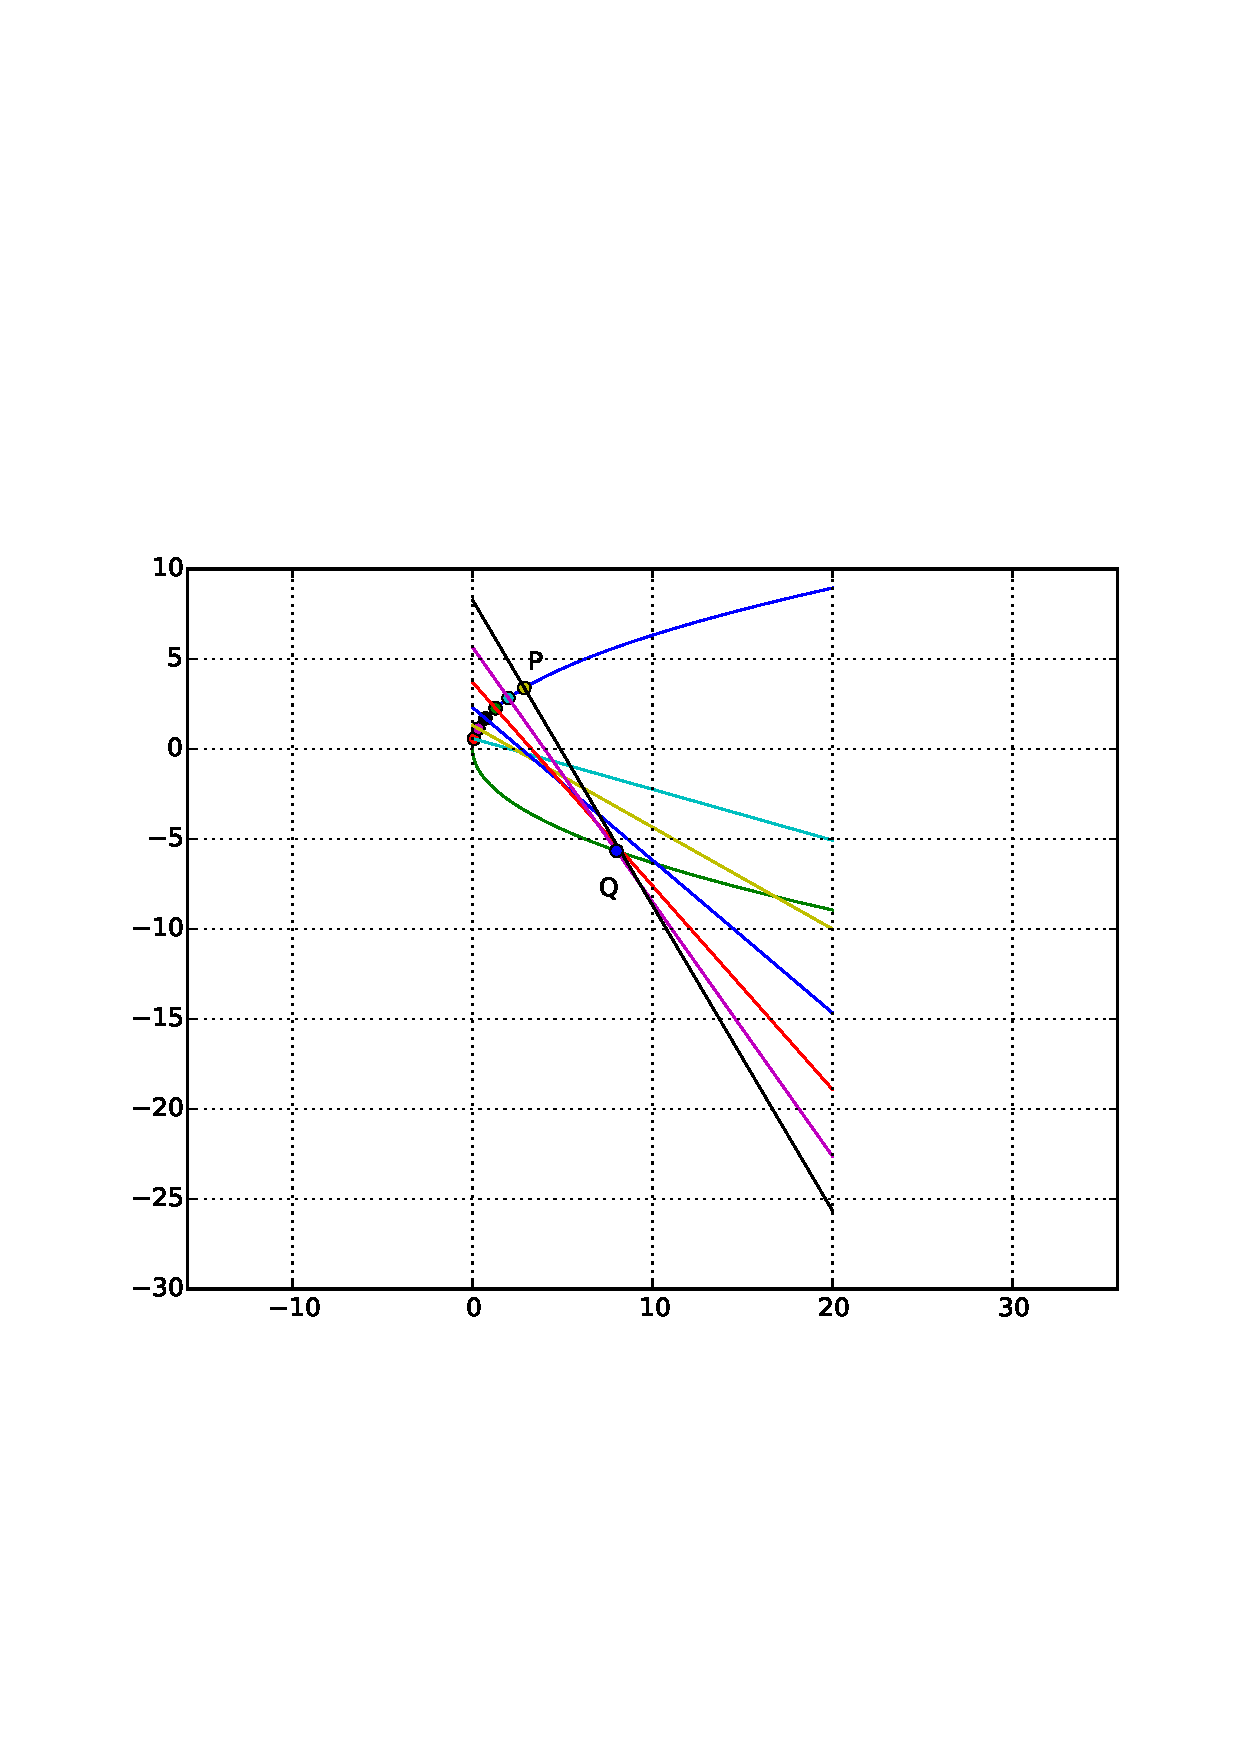
\includegraphics[width=\columnwidth]{./figs/ee16b1023}
\caption{ Normals to the parabola for various values of $t$ plotted.  For $t = \sqrt{2}, t_1 = -2\sqrt{2}, Q\brak{t_1^2 = 8, 2t_1 = -4\sqrt{2}}$ has the smallest $x$-coordinate   among all the normals.}
\label{fig_23}	
\end{figure}
%
\begin{problem}
The transverse axis of a hyperbola is along the major axis of the conic $\frac{x^2}{3}+ \frac{y^2}{4} = 4$. The vertices of the hyperbola are at the foci of this conic. The eccentricity of the hyperbola is $\frac{3}{2}$. Which of the points $\brak{0,2},\brak{\sqrt{5},2\sqrt{2}},\brak{\sqrt{10},2\sqrt{3}},\brak{5, 2\sqrt{3}}$, do not lie on the Hyperbola?
\end{problem}
\solution
%
Let the equation of the ellipse be 
%
\begin{align}
\frac{x^2}{p^2}+ \frac{y^2}{q^2} = 1
\end{align}
%
Then the semi-major and semi-minor axes of the ellipse are $q=4,p = 2\sqrt{3}$ respectively.  The eccentricity of the ellipse is
%
\begin{align}
\varepsilon ={\sqrt {1-\left({\frac {p}{q}}\right)^{2}}} = \frac{1}{2}
\end{align}
%
The foci of the ellipse are at $\brak{0,\pm q\varepsilon}$ on the $y$-axis.  
Let the equation of the hyperbola be
%
\begin{align}
\frac{y^2}{b^2} - \frac{x^2}{a^2} = 1
\end{align}
%
Then $b = q\varepsilon = 2$. Since the eccentricity $e = \frac{3}{2}$, 
%
\begin{equation}
a = b \sqrt{e^2- 1 } = \sqrt{5}
\end{equation}
%
Thus the equation of the desired hyperbola is
%
\begin{align}
\frac{y^2}{4} - \frac{x^2}{5} = 1
\end{align}
%

The following code provides a visualisation of the problem in Fig. \ref{fig_24}.
\lstinputlisting{./codes/ee16b1024.py}
%
\begin{figure}[h]
\centering
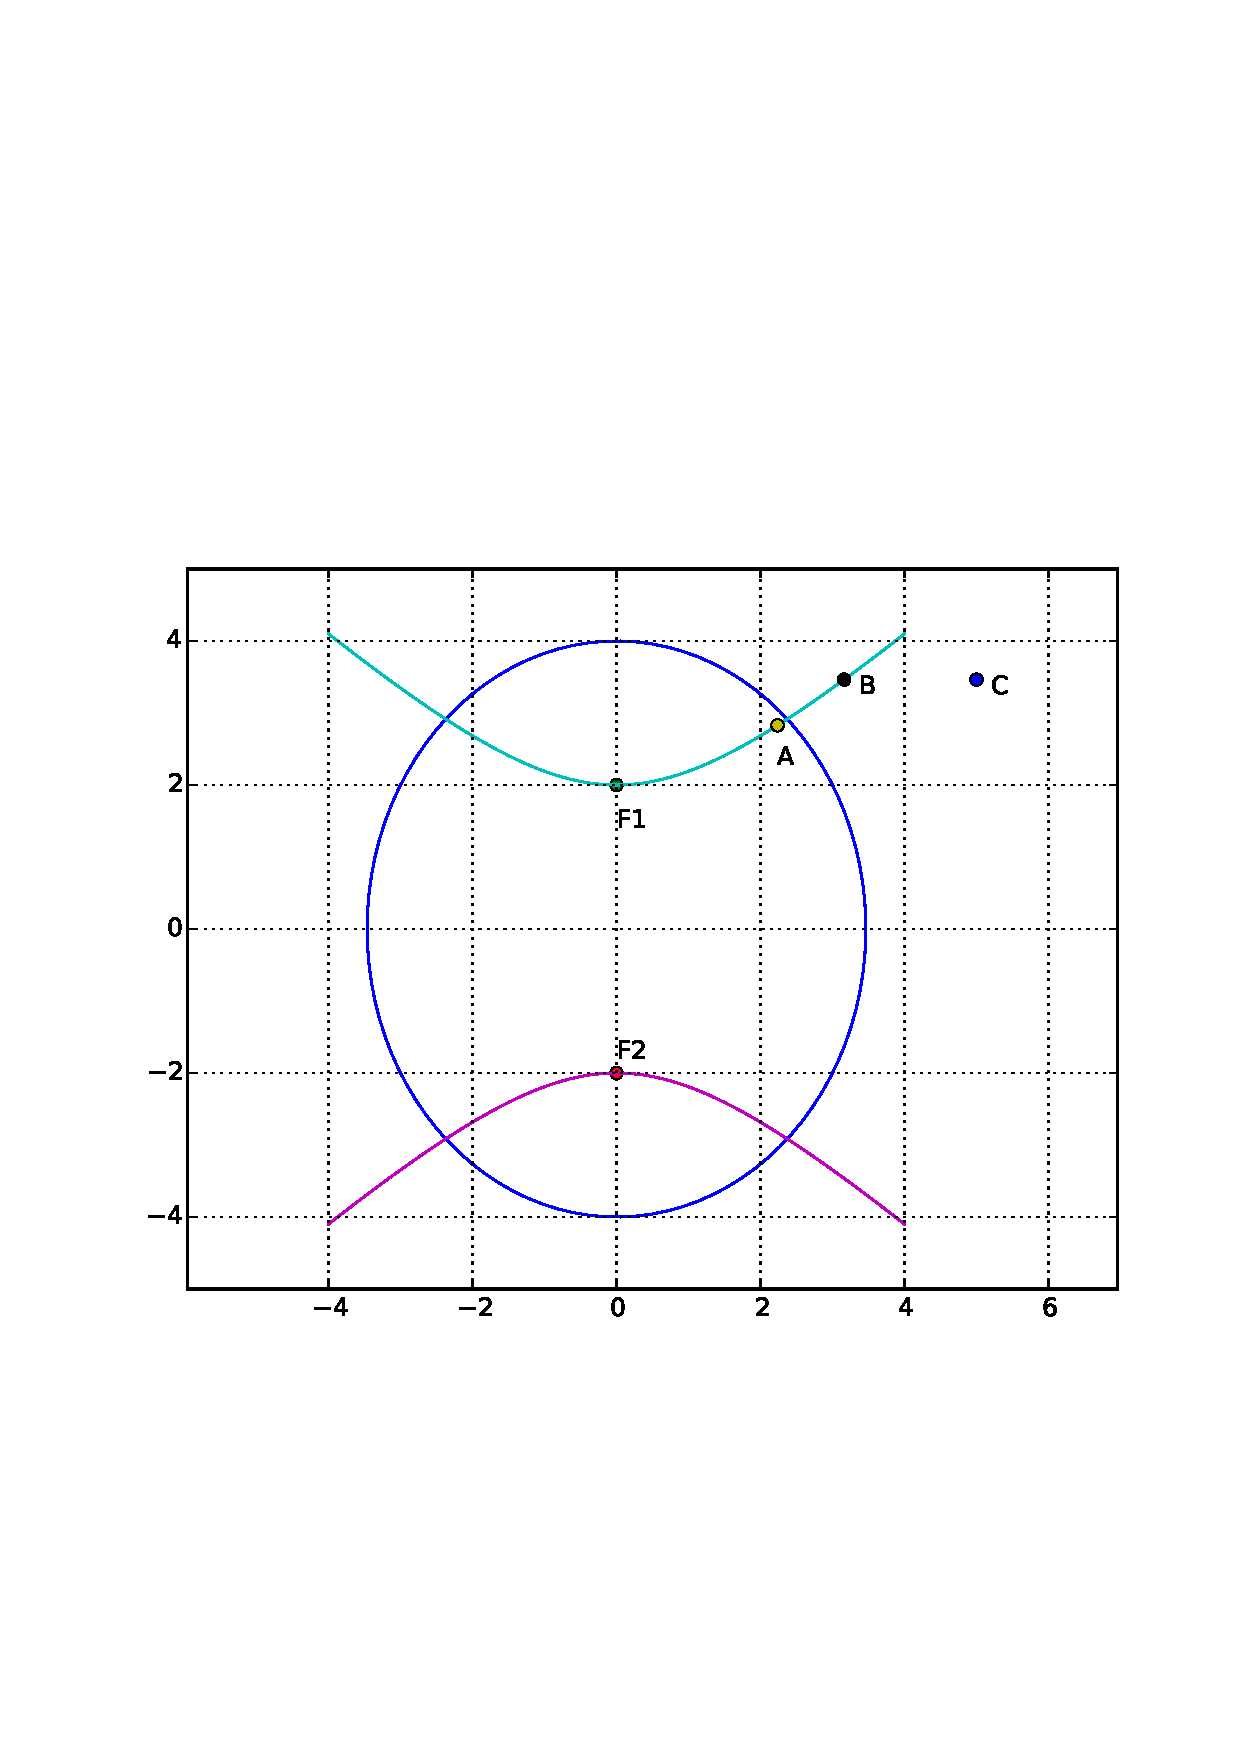
\includegraphics[width=\columnwidth]{./figs/ee16b1024}
\caption{ The point $C$ with coordinates $\brak{5, 2\sqrt{3}}$ does not lie on the hyperbola.}
\label{fig_24}	
\end{figure}
%

\begin{problem}
Find the minimum value of $\tan A + \tan B$, given that $ A+B = \frac{\pi}{6}, A>0,B>0$.
\end{problem}
%
\solution
\begin{align}
\tan A + \tan B &= \frac{\sin A}{\cos A}+\frac{\sin B}{\cos B} \\
	&=\frac{\sin(A+B)}{\cos A \cos B}\\
	&= \frac{2\sin(A+B)}{\cos(A+B)+\cos(A-B)}  \\
	&=\frac{2}{\sqrt{3}+2\cos(A-B)}
\end{align}
$\because A+B = \frac{\pi}{6}$.  The above expression is minimum when 
 $\cos(A-B)$ is $1$, or $A = B = \frac{\pi}{12}$. 
      


The graph is plotted in Fig. \ref{fig_25}
\lstinputlisting{./codes/ee16b1025.py}
%
\begin{figure}[h]
\centering
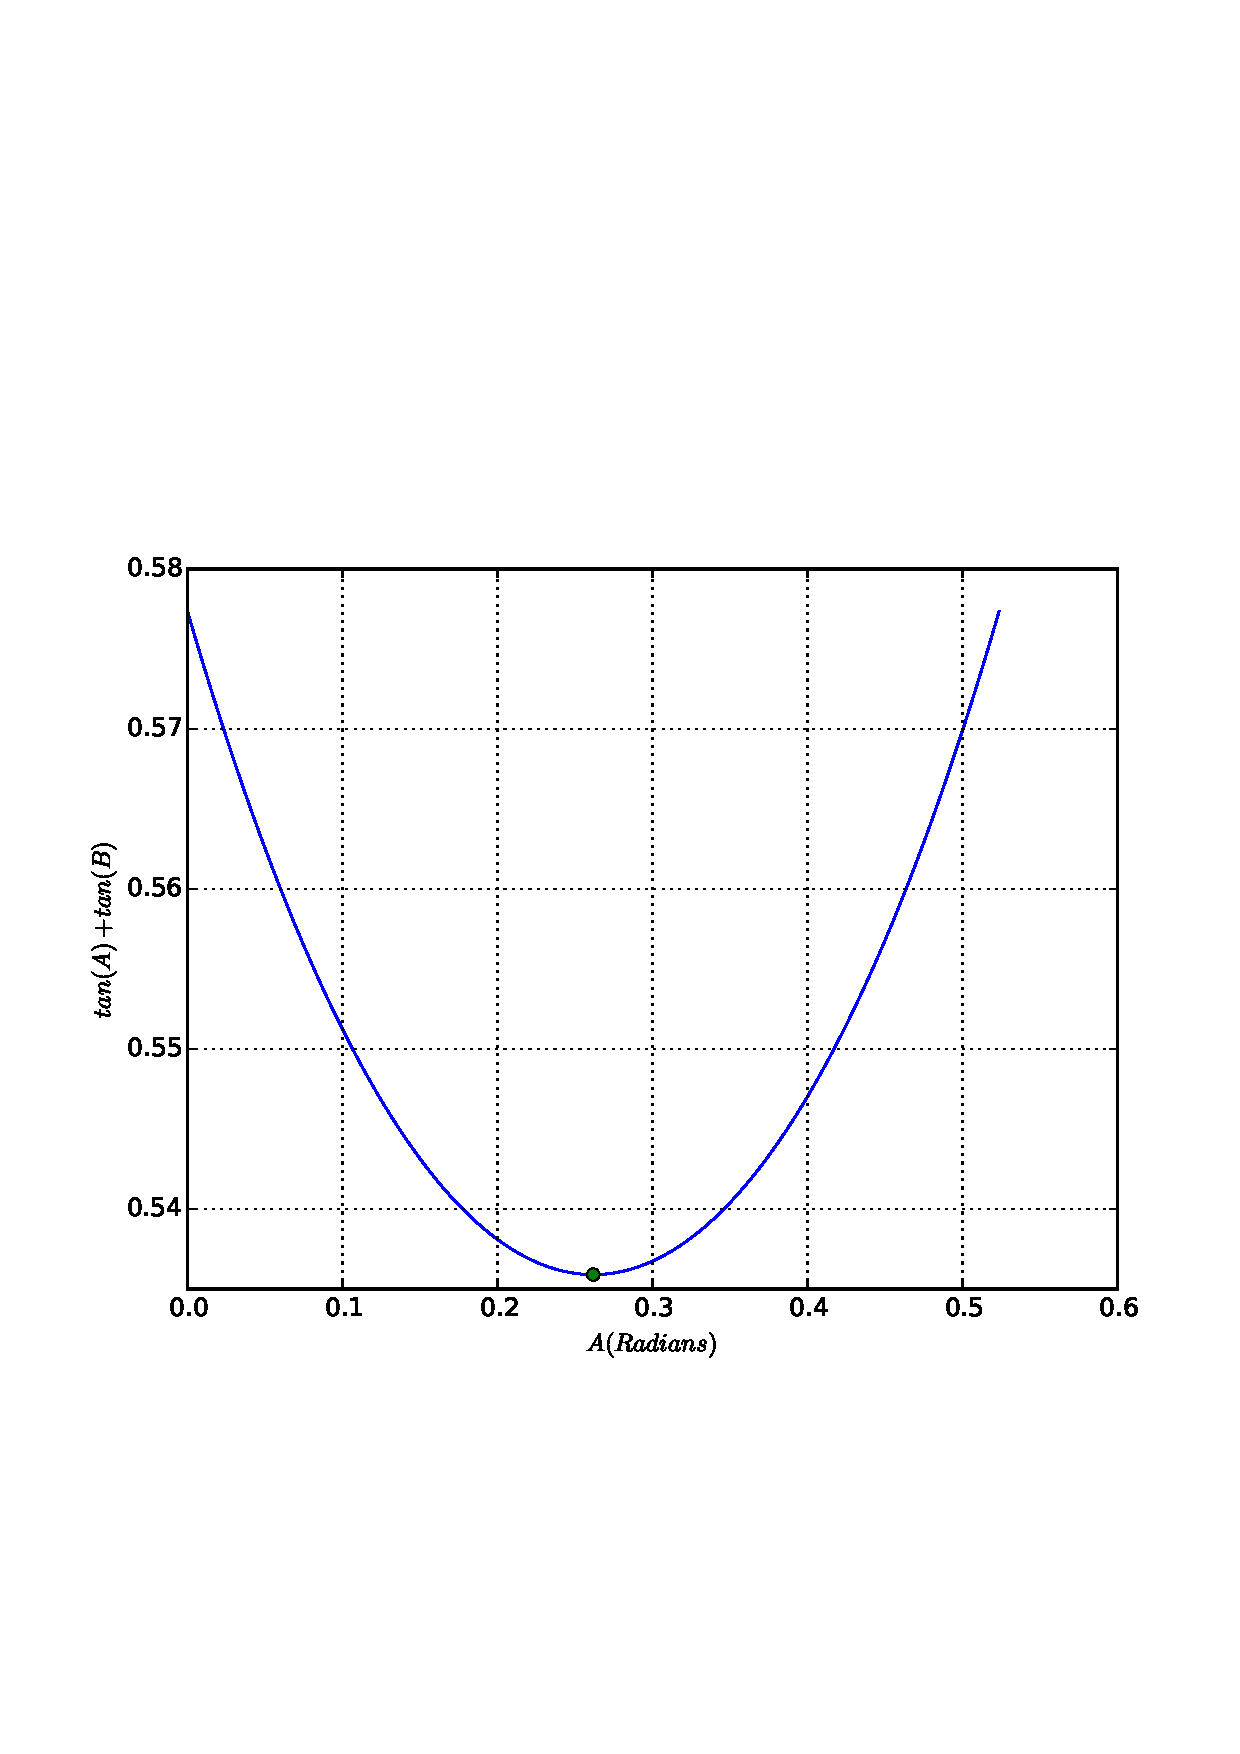
\includegraphics[width=\columnwidth]{./figs/ee16b1025}
\caption{ Finding the minimum of $\tan A + \tan B, A + B = \frac{\pi}{6}$}
\label{fig_25}	
\end{figure}
%
\begin{problem}
Find $\theta$ for which $\frac{2+3\i sin \theta}{1 - 2\i \sin \theta}$ is purely imaginary.
\end{problem}
%
\solution
Simplifying the complex number,
%
\begin{align}
\frac{2+3 \i\sin\theta}{1-2\i\sin\theta} 
&= 
\frac{(2+3\iota\sin\theta)(1+2\iota\sin\theta)}{1+4(\sin\theta)^2}
\\
&=\frac{(2-6\left(\sin\theta\right)^2)+7\iota\sin\theta}{1+4\left(\sin\theta\right)^2}
\end{align}
For the number to be purely iaginary, 
\begin{align}
2-6\left(\sin\theta\right)^2&=0
\Rightarrow
\sin\theta=\pm\frac{1}{\sqrt{3}} 
\\
\Rightarrow 
\theta&=\arcsin{\pm\left(\frac{1}{\sqrt{3}}\right)}   
\end{align}

The graph is plotted in Fig. \ref{fig_26}
\lstinputlisting{./codes/ee16b1026.py}
%
\begin{figure}[h]
\centering
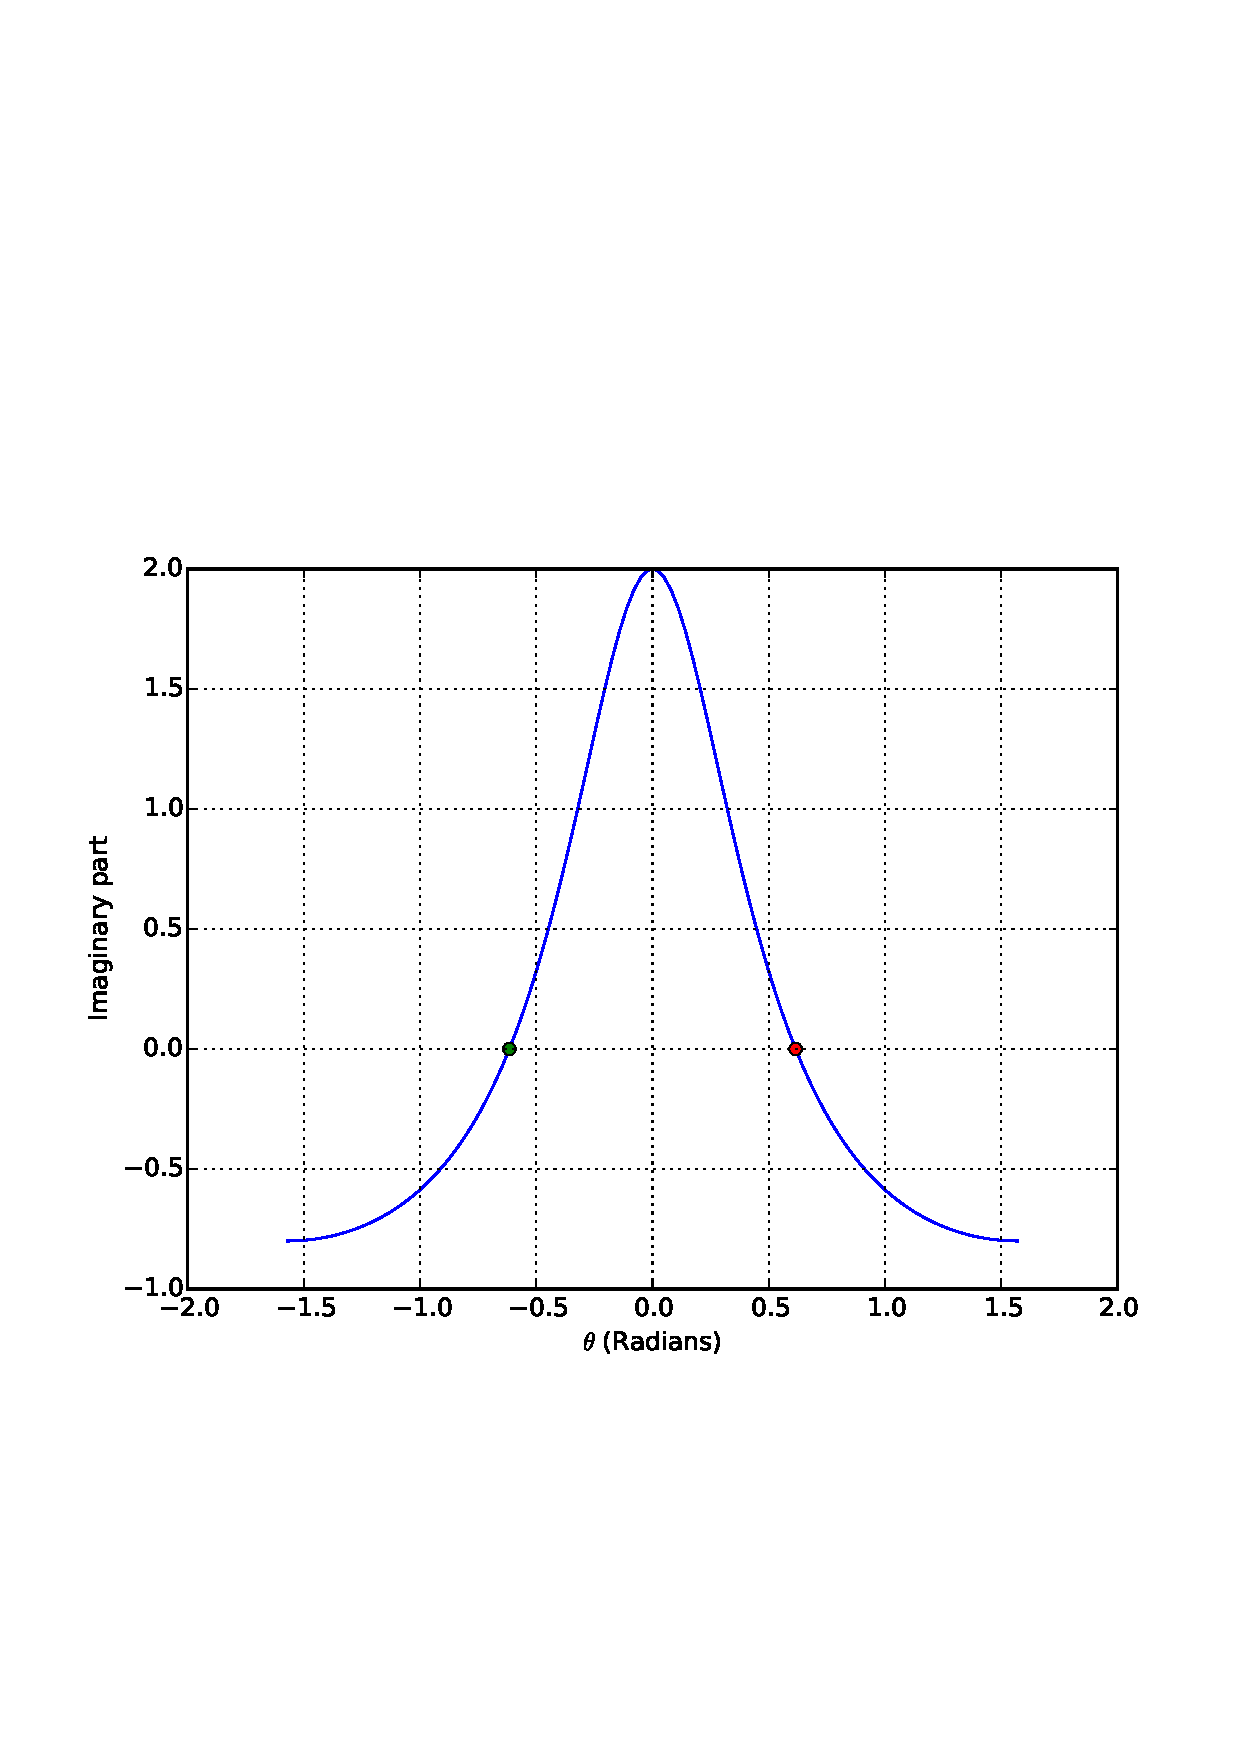
\includegraphics[width=\columnwidth]{./figs/ee16b1026}
\caption{ Complex number is imaginary at $\theta=\arcsin{\pm\left(\frac{1}{\sqrt{3}}\right)}$   }
\label{fig_26}	
\end{figure}
%
\begin{problem}
Find the sum of all the solutions of 
\begin{equation*}
\brak{x^2-5x+5}^{x^2+4x-60}=1
\end{equation*}
\end{problem}
\solution
The solution can be obtained through the following cases
\begin{enumerate}
\item $\left( x^{2}-5x+5 \right) = 1$. This yields the solution 
\begin{equation}
\left( x-1 \right)\left( x-4 \right) = 0 \Rightarrow x = 1,4.
\end{equation}
\item $\left( x^{2}-5x+5 \right) = -1, \left( x^{2}+4x-60 \right)$ even. The first condition yields
%
\begin{align}
\left( x^{2}-5x+6 \right) &= 0
\\
\left( x-3 \right)\left( x-2 \right) &= 0 \Rightarrow x = 3 , 2
\end{align}
Testing the solutions for the second condition,
\begin{equation}
x^2+4x-60
= 
\begin{cases}
-39 & x = 3
\\
-48 & x = 2
\end{cases}
\end{equation}
giving $x =2$ as the desired solution.
%
\item Making the power 0,
\begin{equation}
x^{2}+4x-60 = 0 \Rightarrow x = -10 , 6.
\end{equation}
\end{enumerate}
%
Hence the required solutions are $x=1,4,2,6,-10$ and the sum of these roots is 3.
 

\lstinputlisting{./codes/ee16b1027.py}
%
\begin{problem}
The sum of the first 10 terms of the series $\brak{1\frac{3}{5}}^2+\brak{2\frac{2}{5}}^2+\brak{3\frac{1}{5}}^2+4^2+\brak{4\frac{4}{5}}^2 + \dots $ is $\frac{16}{5}m$.  Find $m$.
\end{problem}
\solution
The given sum can be expressed as
\begin{align}
\left (\frac{4}{5} \right)^{2}\left( 2^{2} + 3^{2} + 4^{2} +.....11^{2} \right) &= \frac{16}{5}m \\
\Rightarrow \brak{\frac{4}{5}}^2\sbrak{\sum_{k = 1}^{11}k^2-1} &= \frac{16}{5}m \\
\Rightarrow \brak{\frac{4}{5}}^2\brak{\frac{11.12.23}{6} - 1} &= \frac{16}{5}m \\
\Rightarrow m = 101
\end{align}


\lstinputlisting{./codes/ee16b1028.py}
%
\begin{problem}
$p = \lim_{x \rightarrow 0+}\brak{1+\tan^2\sqrt{x}}^{\frac{1}{2x}}$. Find  $\log p$.
\end{problem}
\solution 
From the given information,
%
\begin{align}
\log p &= \lim _{x\rightarrow 0+ }\frac{1}{2x}\brak{(1+\tan^{2}{\sqrt{x}}} \\
 &= \frac{1}{2}\lim _{x\rightarrow 0+ }\frac{\tan^{2}{\sqrt{x}}}{\sqrt{x}^2}\frac{1}{\tan^{2}{\sqrt{x}}}\brak{(1+\tan^{2}{\sqrt{x}}}
 \\
 &= \frac{1}{2}
\end{align}
%


The following code verifies this result in Fig. \ref{fig_29}
\lstinputlisting{./codes/ee16b1029.py}
%
\begin{figure}[h]
\centering
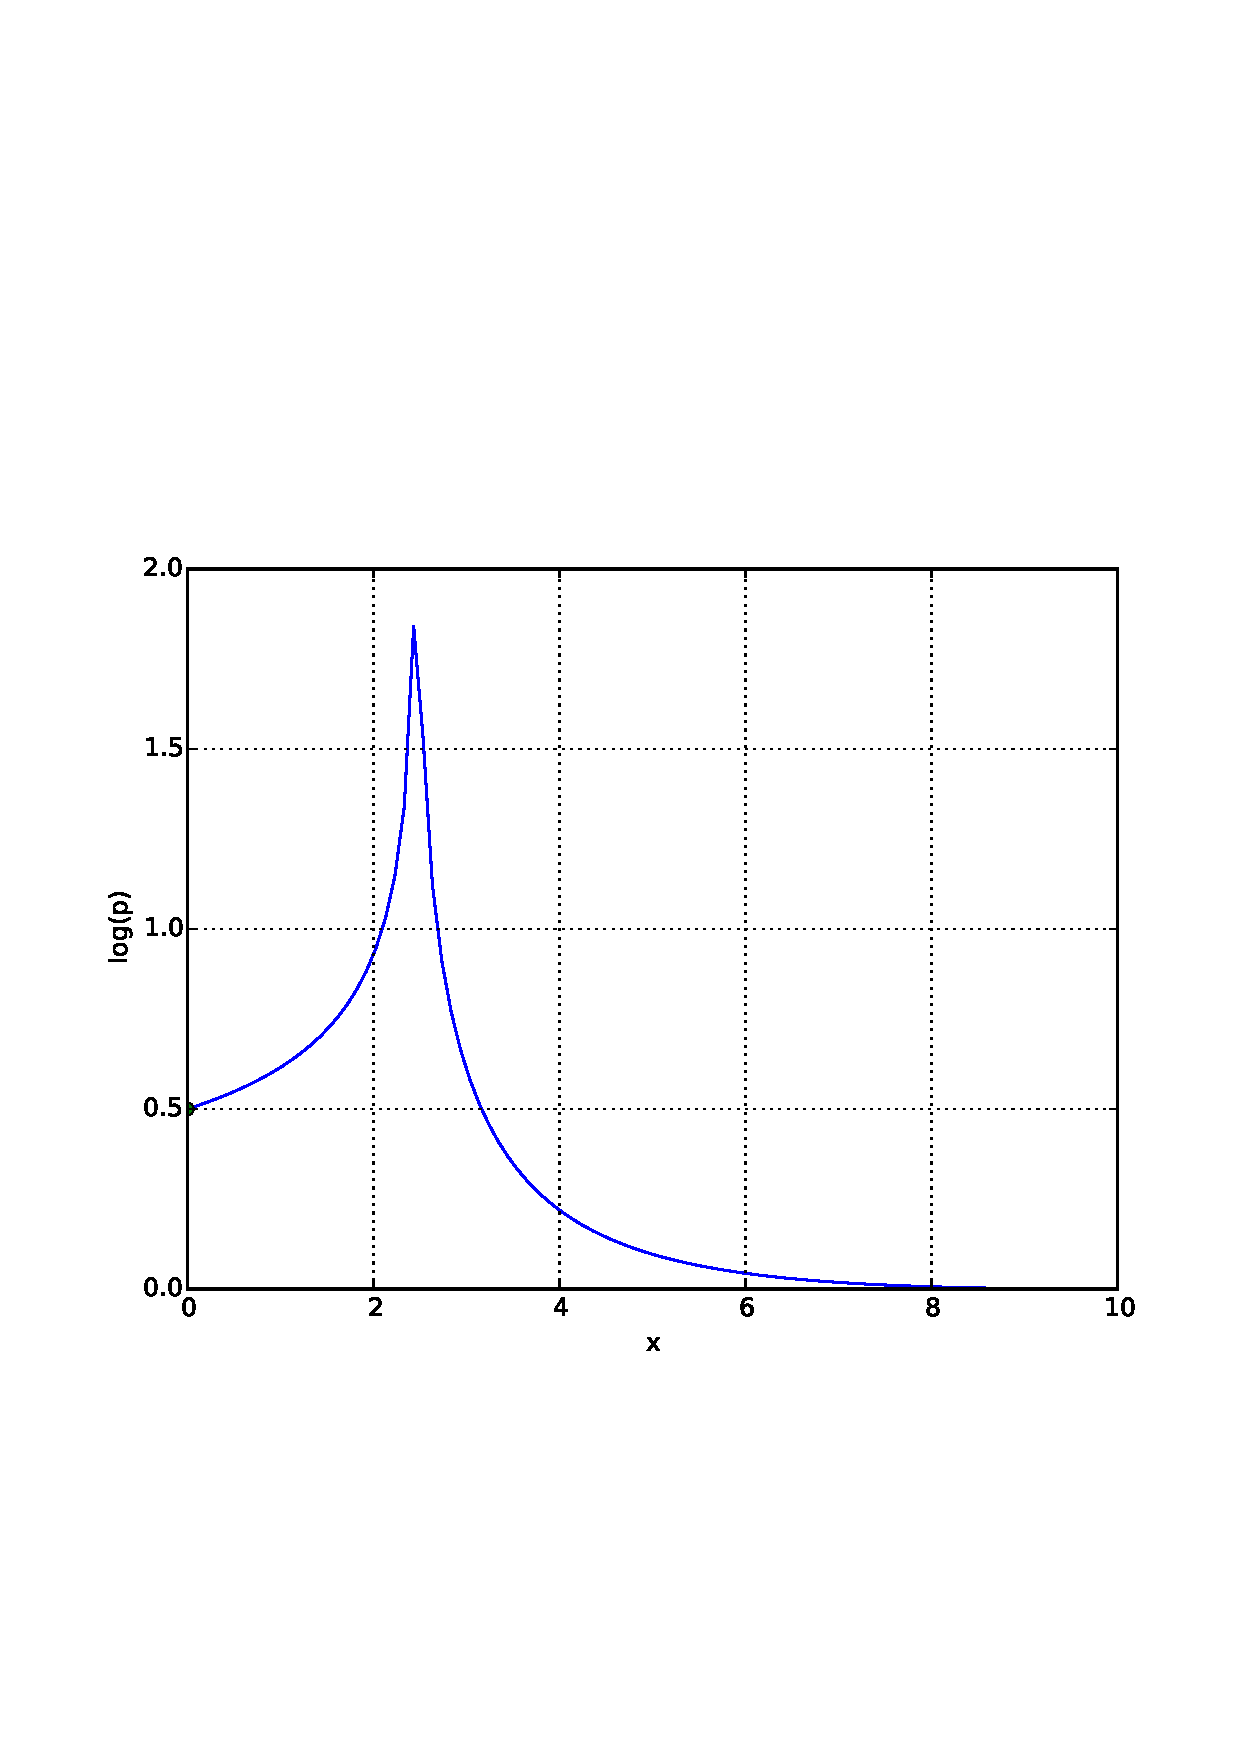
\includegraphics[width=\columnwidth]{./figs/ee16b1029}
\caption{ $\log p = 0.5, x = 0+$}
\label{fig_29}	
\end{figure}
%
\begin{problem}
$f(x) = \abs{\log 2 - \sin x}, x \in \mathbf{R}$ and $g(x)=f(f(x))$.  Which of the following is true?
\begin{enumerate}
\item $g$ is not differentiable at $x=0$
\item $g^{\prime}(0) = \cos \brak{\log 2}$
\item $g^{\prime}(0) = -\cos \brak{\log 2}$
\item $g$ is differentiable at $x=0$ and $g^{\prime }(0) = -\sin \brak{\log 2}$.
\end{enumerate}
\end{problem}
\solution
The function
%
\begin{equation}
g(x)=\abs{\log 2-\sin\abs{\log 2-\sin x}}
\end{equation}
%
Sketching this function in Fig. \ref{fig_30} using the following octave code, it is seen that the function is continuous at $x = 0$.  Computing the right and left hand limits for $g^{\prime}(x)$ at $x = 0$ for $h = 10^{-10}$, the octave code shows that
%
\begin{equation}
\frac{g(h)-g(0)}{h} = \frac{g(0)-g(h)}{h} = \cos(\log 2)
\end{equation}
%


\lstinputlisting{./codes/ee16b1030.py}
%
\begin{figure}[h]
\centering
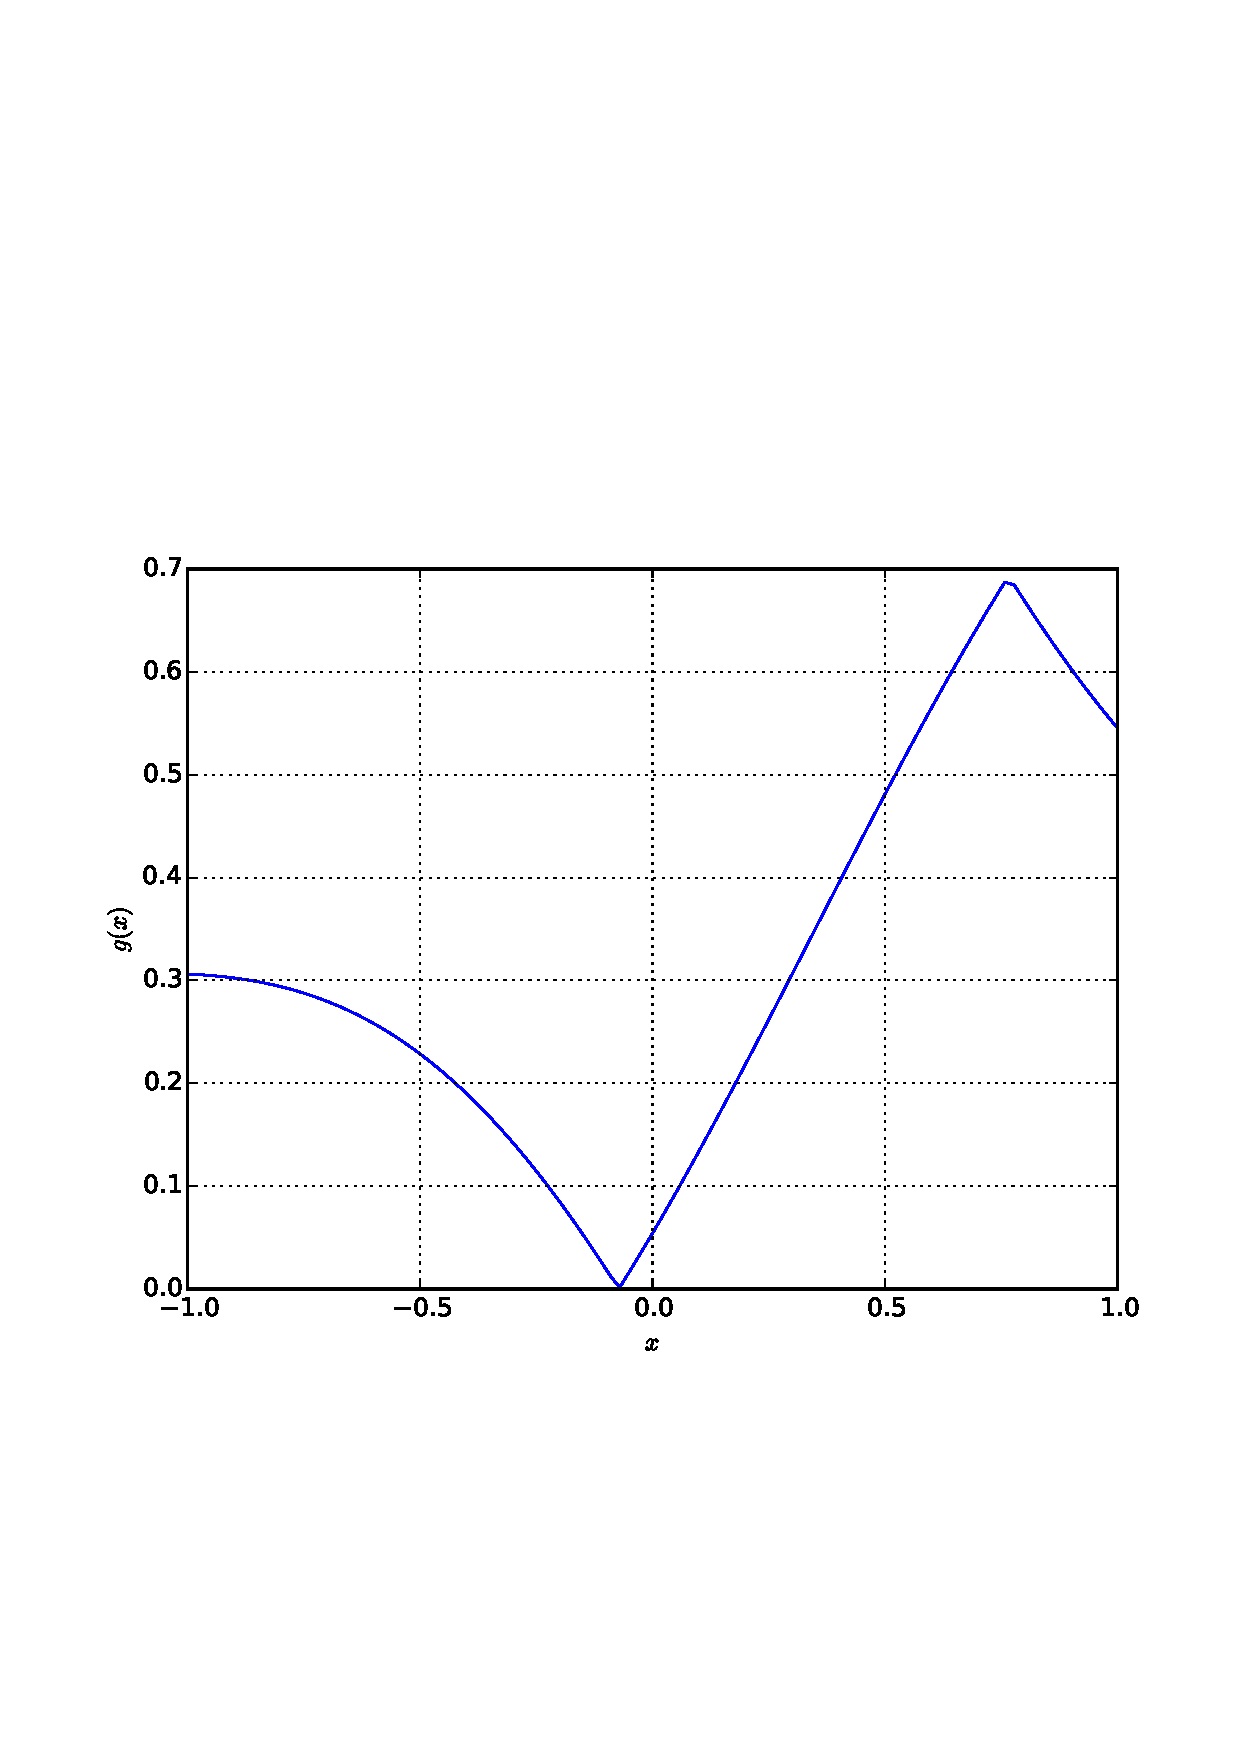
\includegraphics[width=\columnwidth]{./figs/ee16b1030}
\caption{ $g(x)$ continuous at $x = 0$, hence differentialble.  $g^{\prime}(0) = \cos \brak{\log 2}$}
\label{fig_30}	
\end{figure}
%
\begin{problem}
Consider 
\begin{equation*}
f(x) = \tan^{-1}\sqrt{\brak{\frac{1+\sin x }{1-\sin x}}}, x \in \brak{0,\frac{\pi}{2}}
\end{equation*}
Sketch the normal to $f(x)$ at $x = \frac{\pi}{6}$. Does it pass through any of the points $\brak{0,0},\brak{0,\frac{2\pi}{3}},\brak{\frac{\pi}{6},0},\brak{\frac{\pi}{4},0}$?
\end{problem}
The given function can be simplified as
%
\begin{align}
f\left(x\right)&=\tan ^{ -1 }{ \sqrt { \frac { 1+\sin { (x) }  }{ 1-\sin { (x) }  }  }  } \\
&= \tan ^{ -1 } \sqrt { \frac { 2 \cos ^2 \brak{\frac{\pi}{4}-\frac{x}{2}}  }{ 2 \cos ^2 \brak{\frac{\pi}{4}-\frac{x}{2}} }  } \\
& = \tan ^{ -1 } \cot \brak{\frac{\pi}{4}-\frac{x}{2}} \\
& = \frac{\pi}{4}+\frac{x}{2}
\end{align}
%
The normal to $f(x)$ has the equation
%
\begin{equation}
y = -2x + c,
\end{equation}
%
where $c$ is a constant. If $x = \frac{\pi}{6}, f(x) = \frac{\pi}{3}$.  Substituting the coordinates $\brak{\frac{\pi}{6},\frac{\pi}{3}}$ in the equation for the normal, $c = \frac{2\pi}{3}$. 


The normal and the given points are plotted in Fig. \ref{fig_31}.
\lstinputlisting{./codes/ee16b1031.py}
%
\begin{figure}[h]
\centering
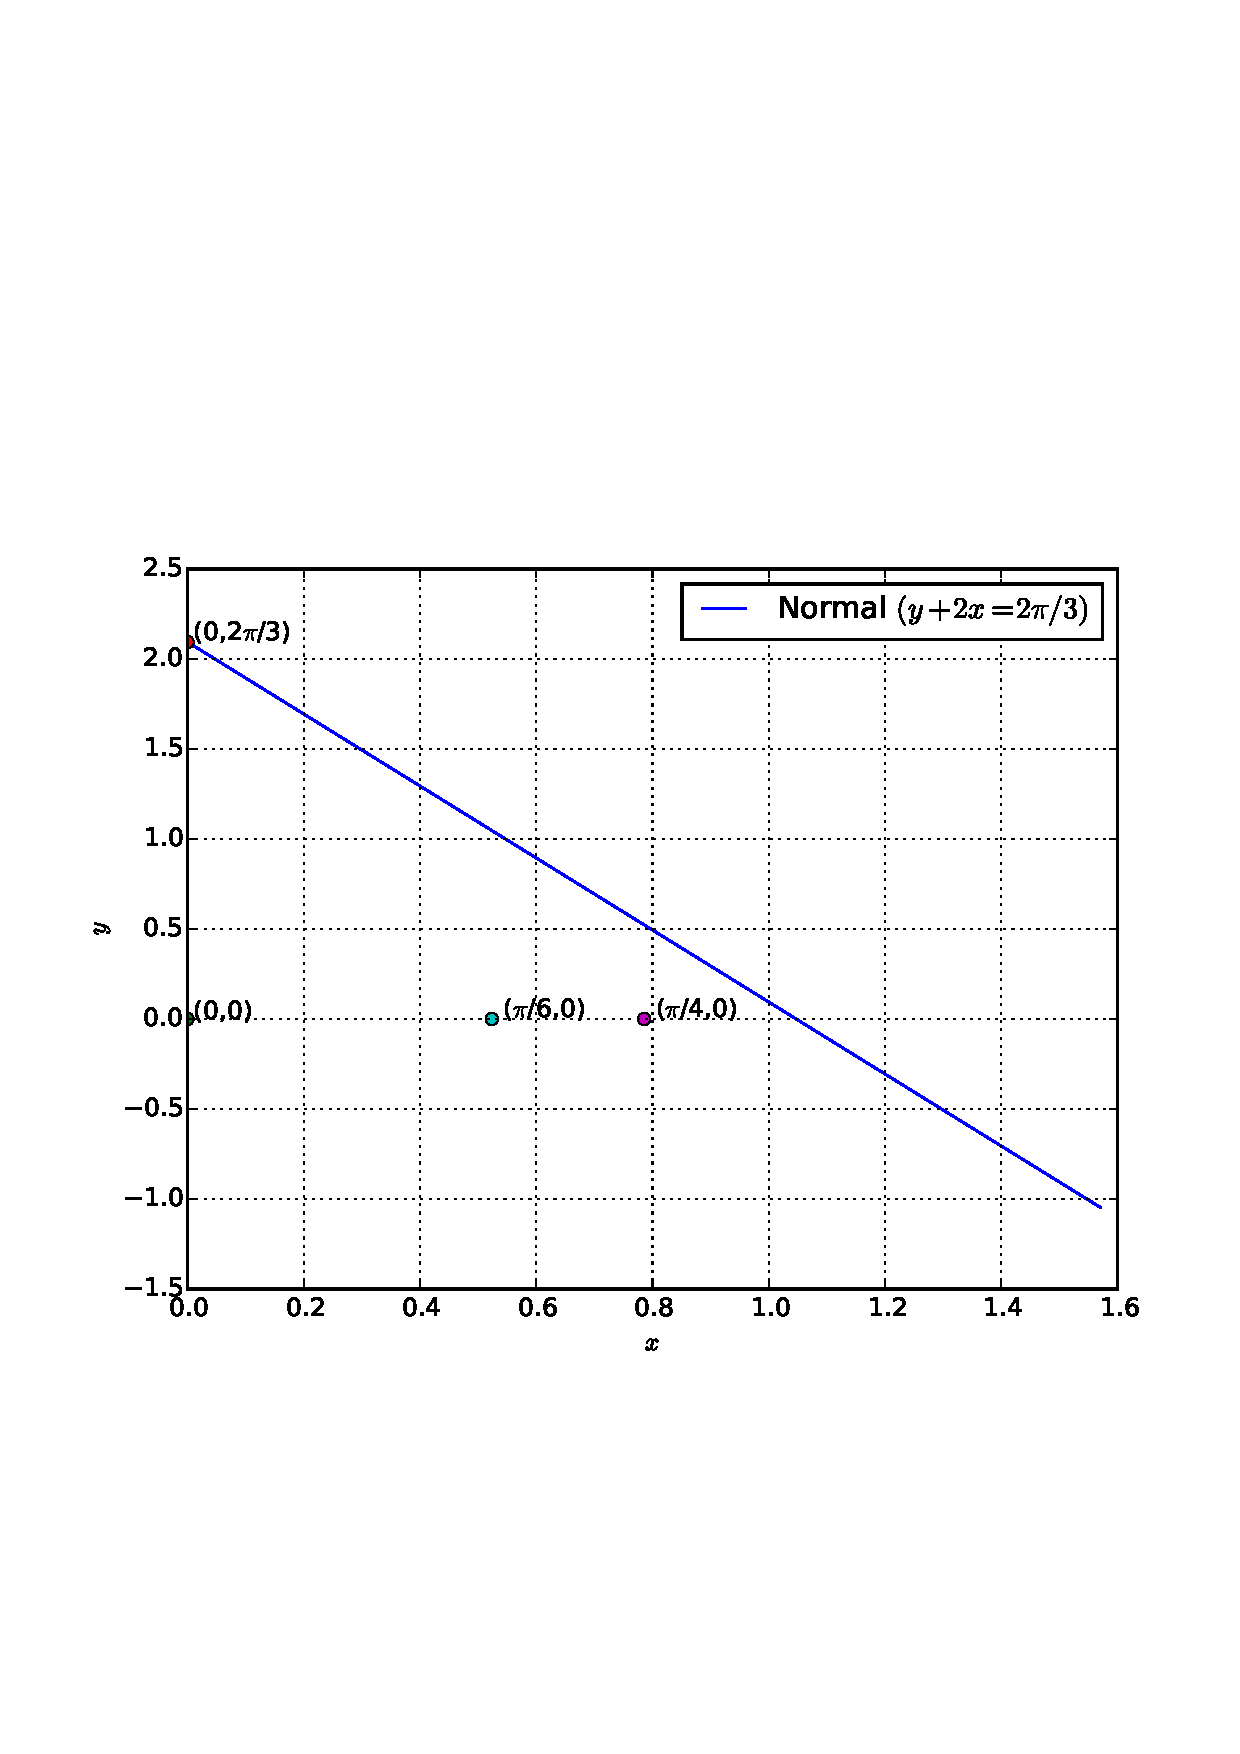
\includegraphics[width=\columnwidth]{./figs/ee16b1031}
\caption{ The normal passes through the point $\brak{0,\frac{2\pi}{3}}$.}
\label{fig_31}	
\end{figure}
%
\begin{problem}
Sketch $\sbrak{\frac{\brak{n+1}\brak{n+2}\dots \brak{3n}}{n^{2n}}}^{\frac{1}{n}}$ and verify if its limit at $n \rightarrow \infty $ is $\frac{18}{e^4},\frac{27}{e^2},\frac{9}{e^2}$ or $3\log 3 -2$.
\end{problem}
\solution	
The given expression can be simplified as
%
\begin{align}
\label{prob32}
p_n = \sbrak{\frac{\brak{n+1}\brak{n+2}\dots \brak{3n}}{n^{2n}}}^{\frac{1}{n}} & = \sbrak{\frac{\brak{3n}!}{n!n^{2n}}}^{\frac{1}{n}}
\end{align}
%
From Stirling's formula, for large $n$,
%
\begin{equation}
 n!\sim {\sqrt {2\pi n}}\left({\frac {n}{e}}\right)^{n}.
\end{equation}
%
Substituting the above in \eqref{prob32},
%
\begin{align}
\sbrak{\frac{\brak{3n}!}{n!n^{2n}}}^{\frac{1}{n}} & = \sbrak{\frac{{\sqrt {2\pi \brak{3n}}}\left({\frac {3n}{e}}\right)^{3n}}{{\sqrt {2\pi n}}\left({\frac {n}{e}}\right)^{n}.n^{2n}}}^{\frac{1}{n}}
\\
&= \sbrak{\frac{\sqrt{3}\brak{3}^{3n}}{e^{2n}}}^{\frac{1}{n}} = \frac{27}{e^2}
\end{align}
%
in the limit.

This solution agrees with the plot of $p_n$ shown in Fig. \ref{fig_32}.
\lstinputlisting{./codes/ee16b1032.py}
%
\begin{figure}[h]
\centering
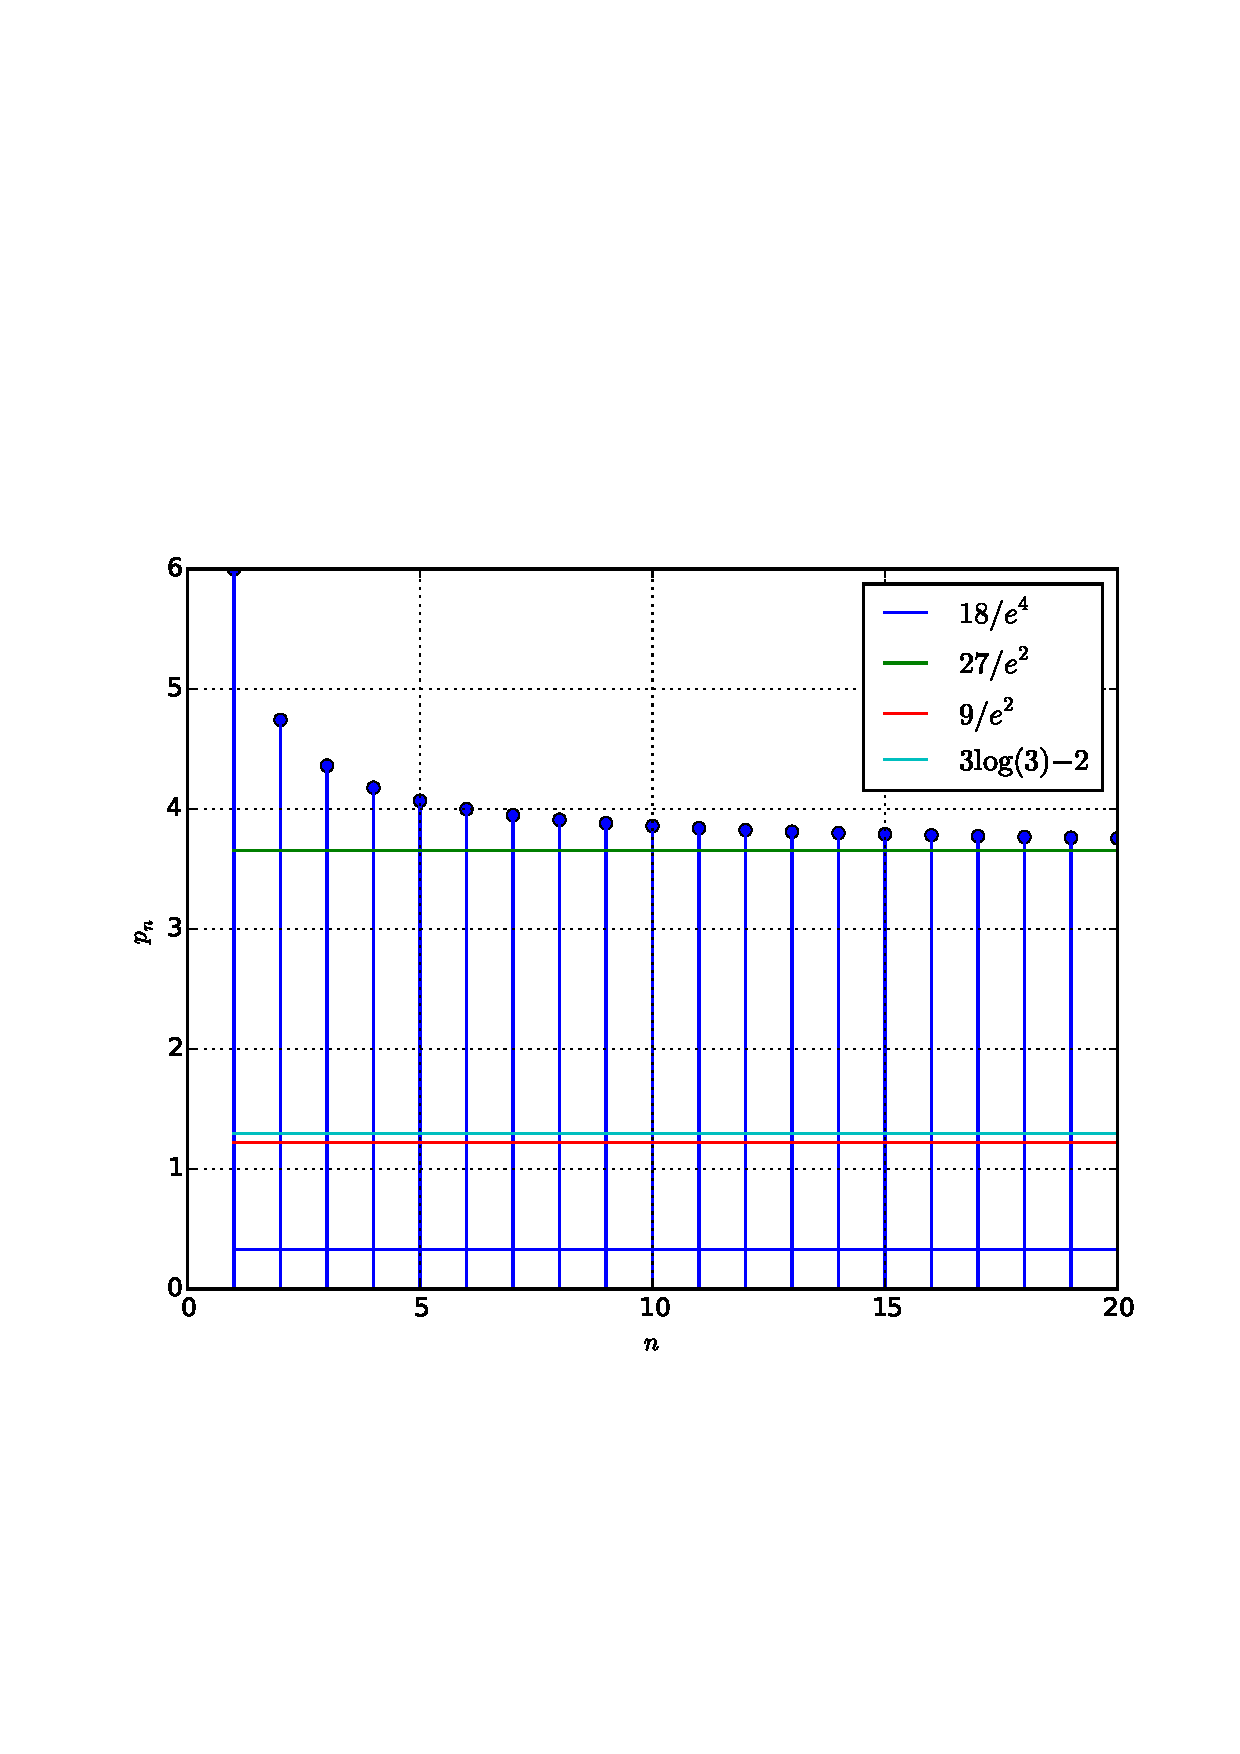
\includegraphics[width=\columnwidth]{./figs/ee16b1032}
\caption{ In the limit, the expression converges to $\frac{27}{e^2}$}
\label{fig_32}	
\end{figure}
%
\begin{problem}
Sketch the region 
\begin{equation*}
\cbrak{\brak{x,y}: y^2 \geq 2x, x^2+y^2 \leq 4x, x \geq 0, y \geq 0 }
\end{equation*}
\end{problem}
\solution
The following code plots the desired region in Fig. \ref{fig_33}.
\lstinputlisting{./codes/ee16b1033.py}
%
\begin{figure}[h]
\centering
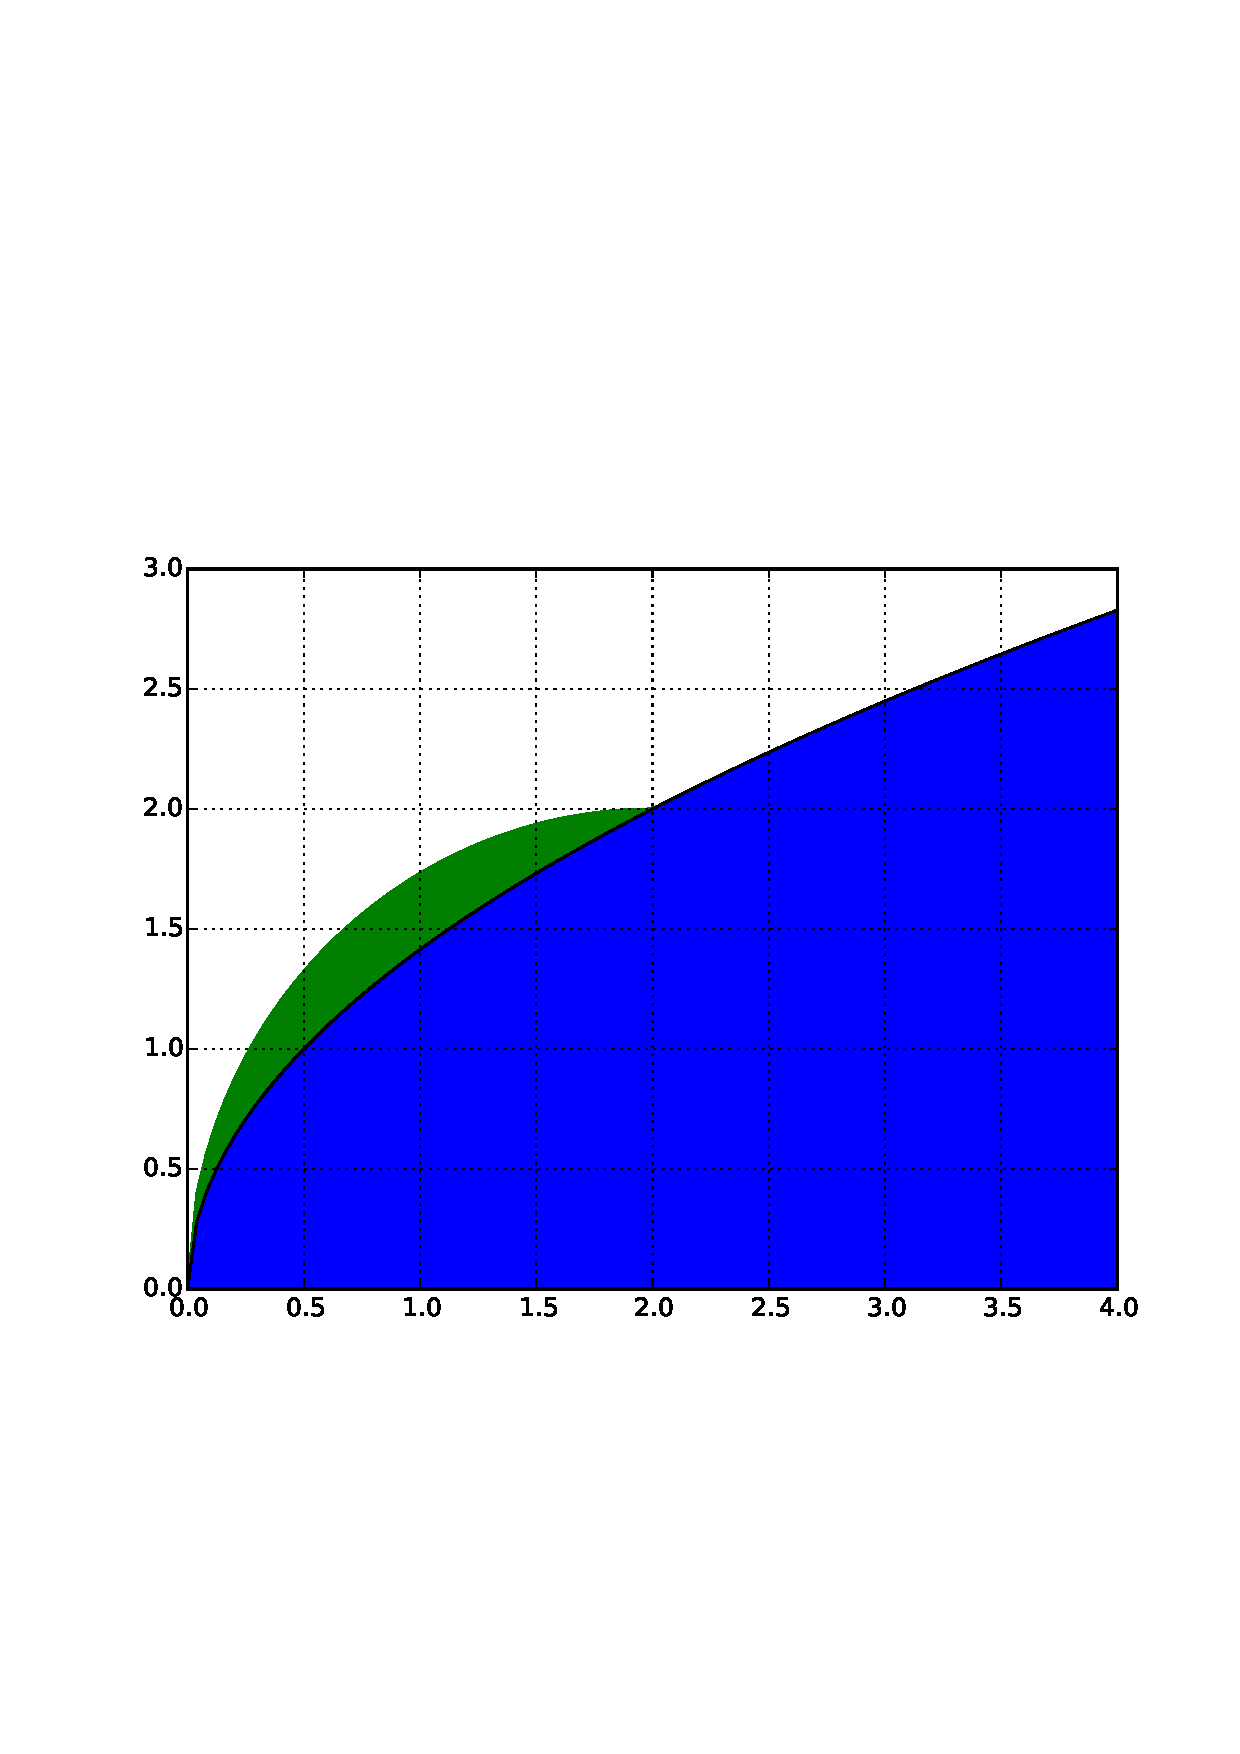
\includegraphics[width=\columnwidth]{./figs/ee16b1033}
\caption{ Desired region is in green colour}
\label{fig_33}	
\end{figure}
%
\begin{problem}
Two sides of a rhombus are along the lines $x-y+1 = 0$ and $7x-y-5=0$. Its diagonals intersect at $\brak{-1,-2}$. Find the vertices of the rhombus.
\end{problem}
\solution
The point of intersection of the two lines is one vertex of the rhombus.  This point is obtained by soving the following matrix equation 
%
\begin{equation}
\begin{pmatrix}
1 & -1
\\
7 & -1
\end{pmatrix}
\mbf{x} = 
\begin{pmatrix}
-1
\\
5
\end{pmatrix}
\end{equation}
%
using the octave code to obtain the point $P$ $\brak{1,2}$.  Since diagonals of a rhombus bisect each other and the point of intersection $O$ is given as $\brak{-1,-2}$ the coordinates of the opposite vertex $R$ are given by 
%
\begin{equation}
\mathbf{x} + 
\begin{pmatrix}
1 
\\
2
\end{pmatrix}
= 
2
\begin{pmatrix}
-1 
\\
-2
\end{pmatrix} \Rightarrow \mbf{x} = 
\begin{pmatrix}
-3
\\
-6
\end{pmatrix}
\end{equation}
%
Since the sides of a rhombus are equal, if the unknown vertex $Q$ has coordinates $\brak{x,y}$,
\begin{align}
PQ = QR \Rightarrow \brak{x-1}^2 + \brak{y-2}^2 &= \brak{x+3}^2  + \brak{y+6}^2 \nonumber \\
\Rightarrow x + 2 y &= -5 
\end{align}
Note that the above locus is actually the diagonal $QS$.  Letting $PQ$ be
\begin{equation}
x-y+1 = 0,
\end{equation}
%
$Q$ is obtained from the following equation
%
%
\begin{equation}
\begin{pmatrix}
1 & 2
\\
1 & -1
\end{pmatrix}
\mbf{x} = 
\begin{pmatrix}
-5
\\
-1
\end{pmatrix}
\end{equation}
%
as $\brak{-\frac{7}{3},-\frac{4}{3}}$.
%
Similarly, letting $PS$ to be
%
\begin{equation}
7x-y-5=0,
\end{equation}
%
$S$ is obtained from the equation
%
\begin{equation}
\begin{pmatrix}
1 & 2
\\
7 & -1
\end{pmatrix}
\mbf{x} = 
\begin{pmatrix}
-5
\\
5
\end{pmatrix}
\end{equation}
%
as $\brak{\frac{1}{3},-\frac{8}{3}}$.



Fig. \ref{fig_34} explains the problem.
\lstinputlisting{./codes/ee16b1034.py}
%
\begin{figure}[h]
\centering
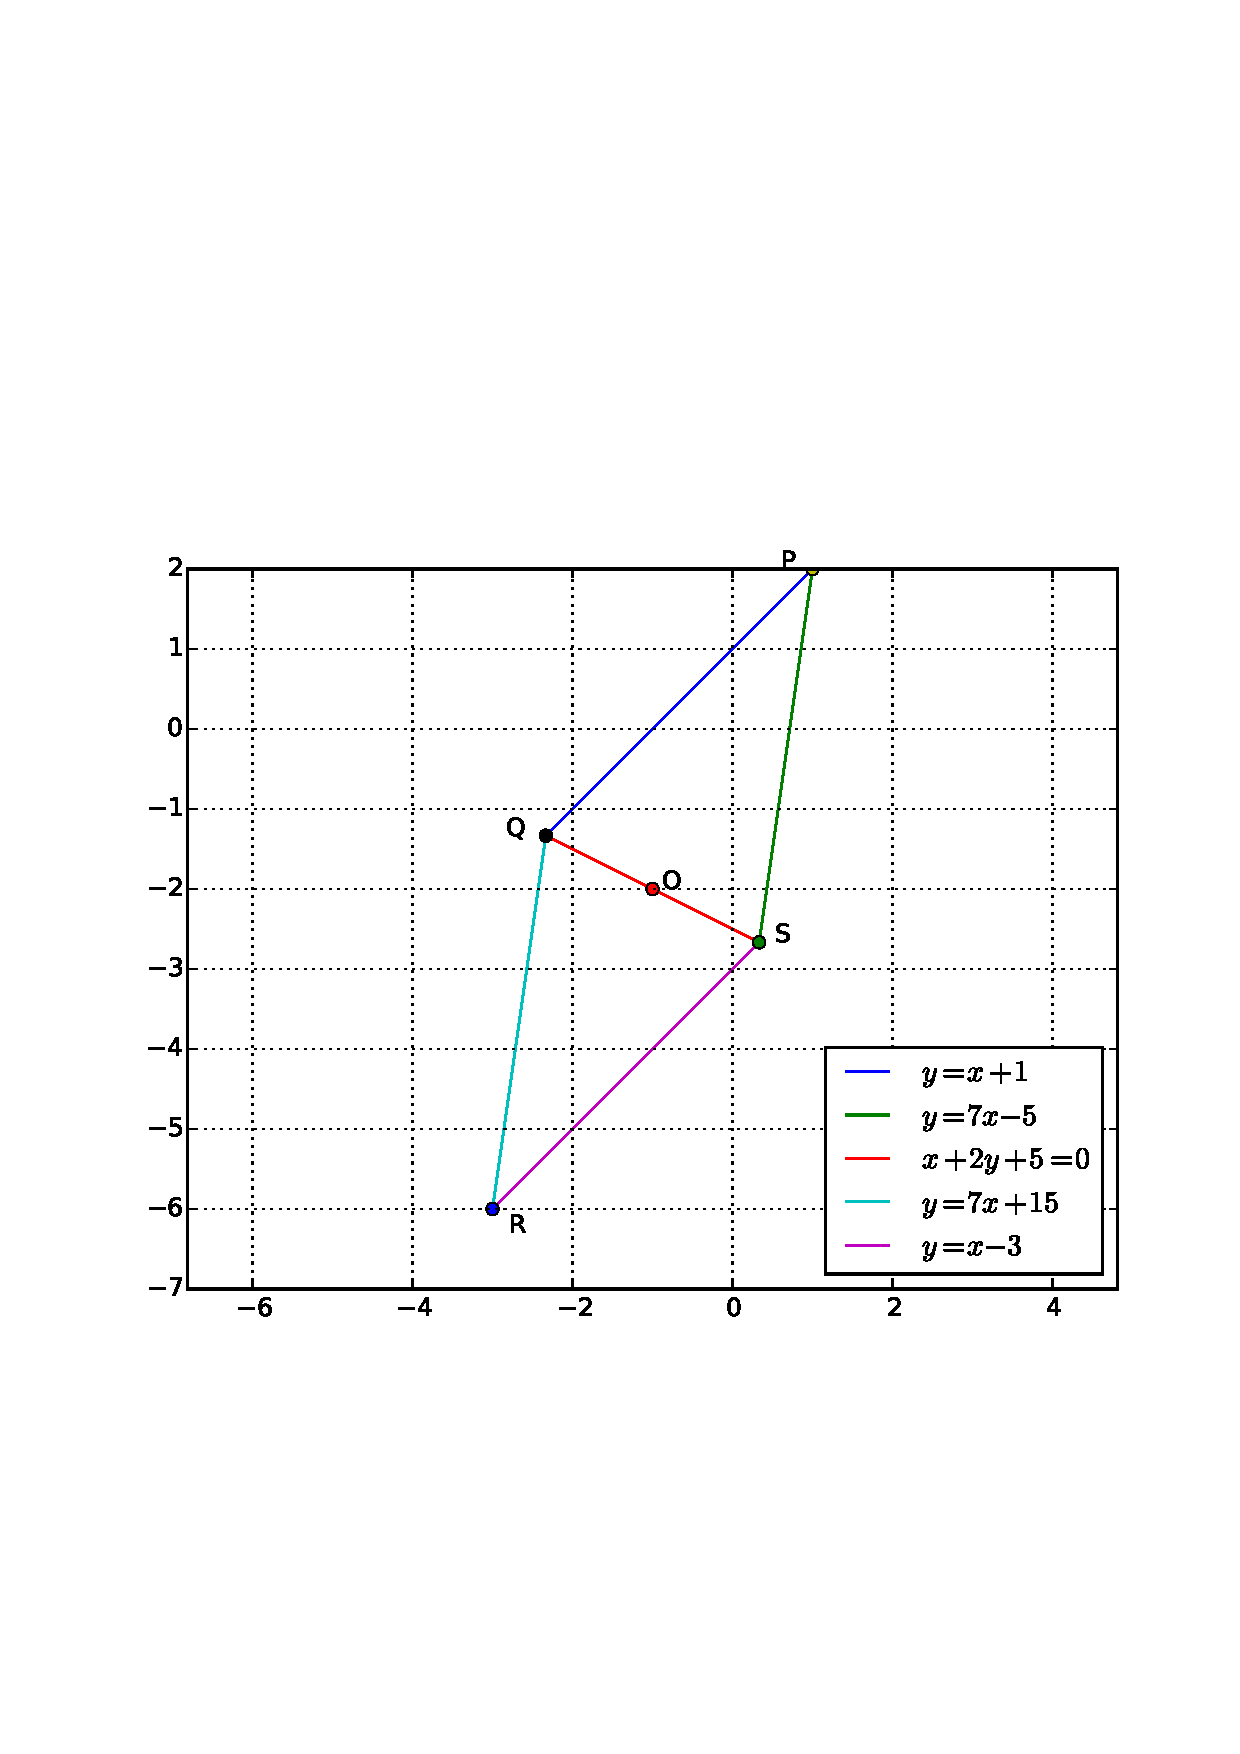
\includegraphics[width=\columnwidth]{./figs/ee16b1034}
\caption{ Desired rhombus.}
\label{fig_34}	
\end{figure}
%
\begin{problem}
Sketch the locus of the centres of circles which touch the circle $x^2+y^2-8x-8y-4=0$ as well as the $x-$axis. 
\end{problem}
\solution
The given circle can be expressed in standard form as
%
\begin{equation}
\brak{x-4}^2 + \brak{y-4}^2 = 6^2
\end{equation}
%
i.e., the cricle has centre at $\brak{4,4}$ and radius 6.
Let $\brak{h,k}$ be the centre of a circle that touches the given circle. Since this  circle touches the $x$-axis, its radius is $k$. This circle can touch the given circle internally or externally.
\begin{enumerate}
\item {\em External:}  In this case, sum of radius of two circles is equal to distance between them.  Hence, 
%
\begin{align}
|k|+6&=\sqrt{(h-4)^{2}+(k-4)^{2}}
\\
\Rightarrow k^2 + 12\abs{k} + 36 &= \brak{h-4}^2 + k^2 -8k + 16 \\
\Rightarrow  12\abs{k} +8k &= \brak{h-4}^2 - 20\\
\Rightarrow  k &= 
\begin{cases}
\frac{\brak{h-4}^2 - 20}{20} & k  > 0
\\
-\frac{\brak{h-4}^2 - 20}{4} & k < 0
\end{cases}
\end{align}
%
\item {\em Internal:} Modulus of difference of radius of two circles is equal to distance between them.  hence
%
\begin{align}
\abs{|k|-6}&=\sqrt{(h-4)^{2}+(k-4)^{2}}
\\
\Rightarrow k^2 - 12\abs{k} + 36 &= \brak{h-4}^2 + k^2 -8k + 16 \\
\Rightarrow  -12\abs{k} +8k &= \brak{h-4}^2 - 20\\
\Rightarrow  k &= 
\begin{cases}
\frac{\brak{h-4}^2 - 20}{20} & k  < 0
\\
-\frac{\brak{h-4}^2 - 20}{4} & k > 0
\end{cases}
\end{align}
%
\end{enumerate}
%
Both the above cases can be combined to obtain the locus as the curves
%
\begin{align}
y &= \frac{\brak{x-4}^2 }{20} - 1
\\
y &= 5 - \frac{\brak{x-4}^2 }{4} 
\end{align}
%

\lstinputlisting{./codes/ee16b1035.py}
%
\begin{figure}[h]
\centering
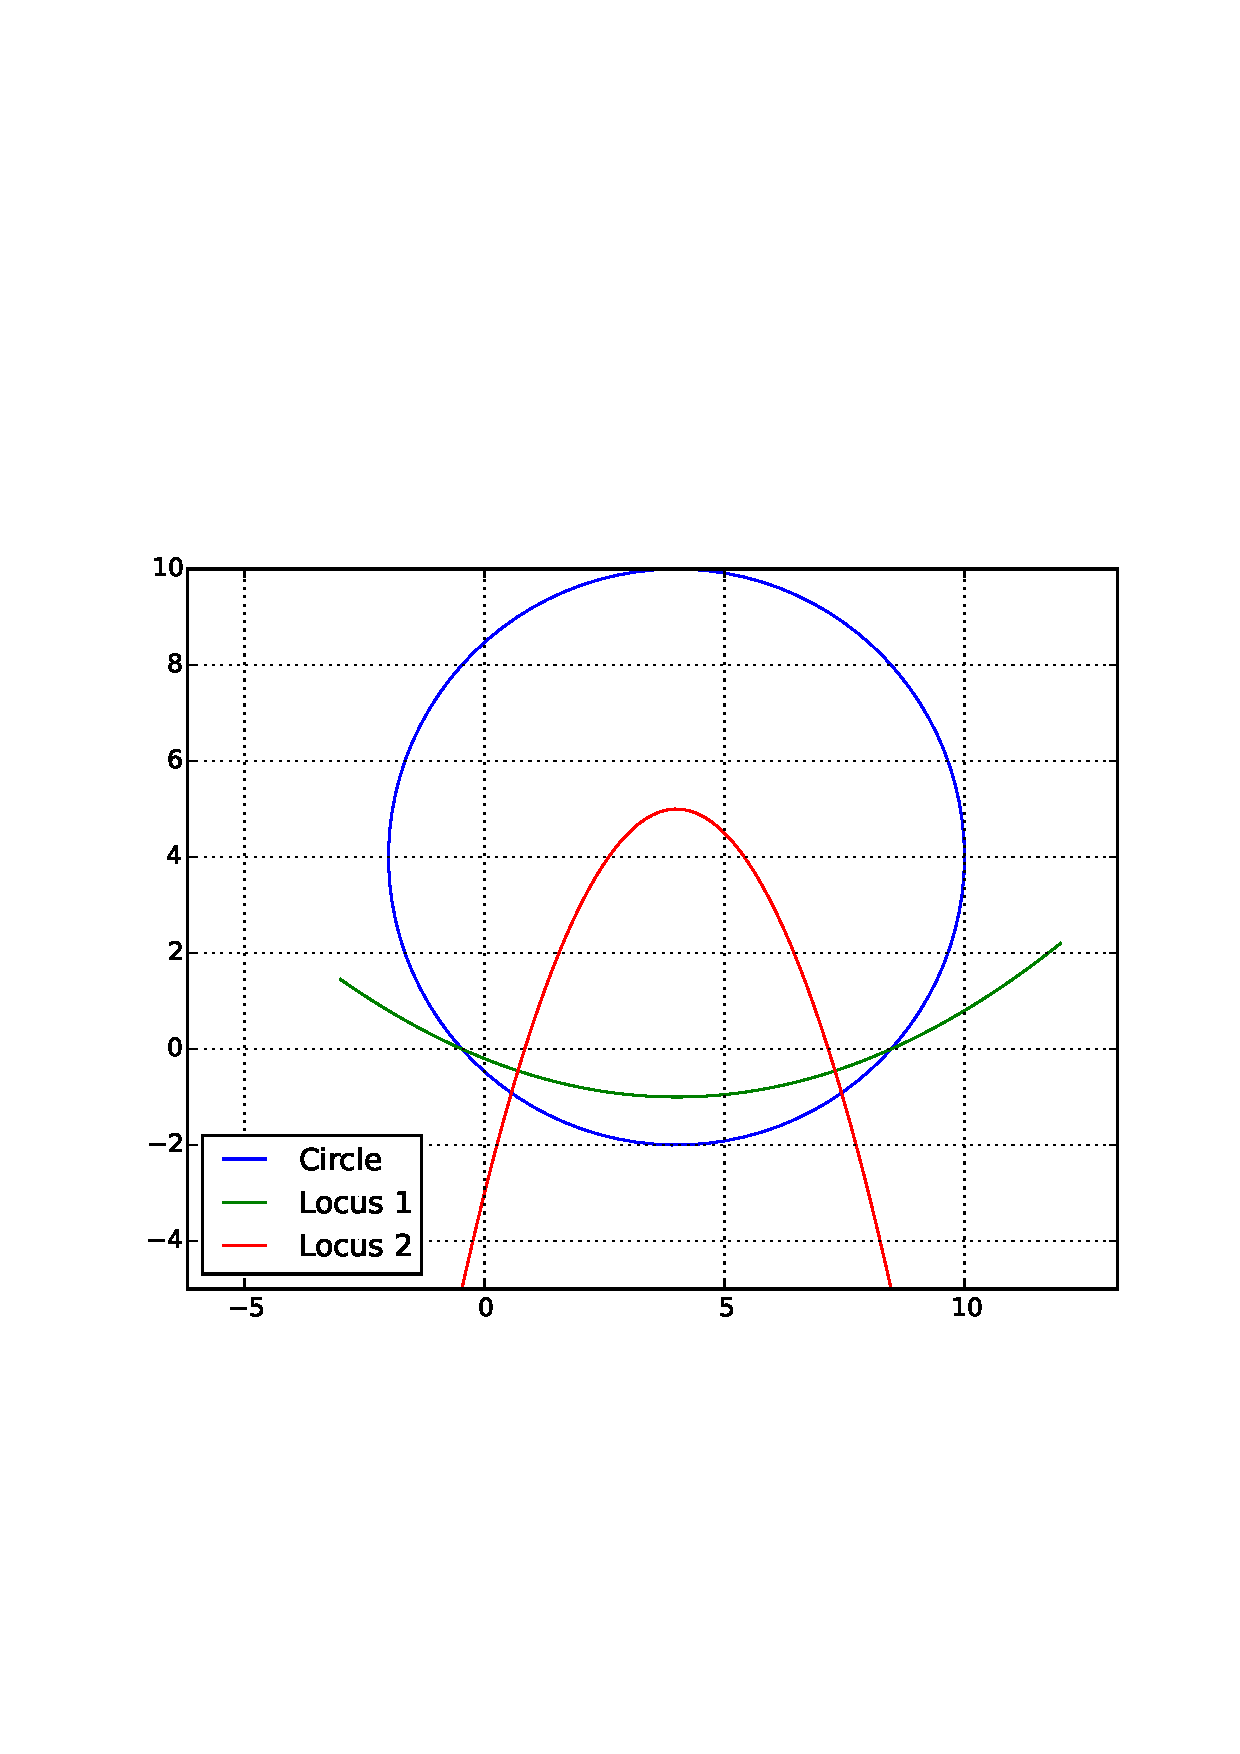
\includegraphics[width=\columnwidth]{./figs/ee16b1035}
\caption{ Required loci.}
\label{fig_35}	
\end{figure}
%
\begin{problem}
One of the diameters of the  circle $x^2+y^2-4x+6y-12 = 0$ is a chord of a circle $S$. The centre of $S$ is at $\brak{-3,2}$. Sketch $S$ and find its radius.
\end{problem}
\solution
The given circle can be expressed in standard form as
%
\begin{equation}
\brak{x-2}^2 + \brak{y+3}^2 = 5^2
\end{equation}
%
i.e., the circle has centre at $O$ with coordinates $\brak{2,-3}$ and radius 5. Using the distance formula, $OS = 5\sqrt{2}.  $Let the radius of the circle with centre at $S$ be $r$. $r$ can be obtained using Budhayana's theorem as 
%
\begin{align}
r^2 &= 5^2 + OS^2 
\\
\Rightarrow r &= 5 \sqrt{3}
\end{align}
% 
The diameter of the circle with centre $O$ and chord of circle with centre $S$ is perpendicular to OS. The equation of the diameter is thus obtained as
%
\begin{align}
\brak{y + 3} = \brak{x-2} \Rightarrow y = x -5
\end{align}
%

Fig. \ref{fig_36} summarises the problem.
\lstinputlisting{./codes/ee16b1036.py}
%
\begin{figure}[h]
\centering
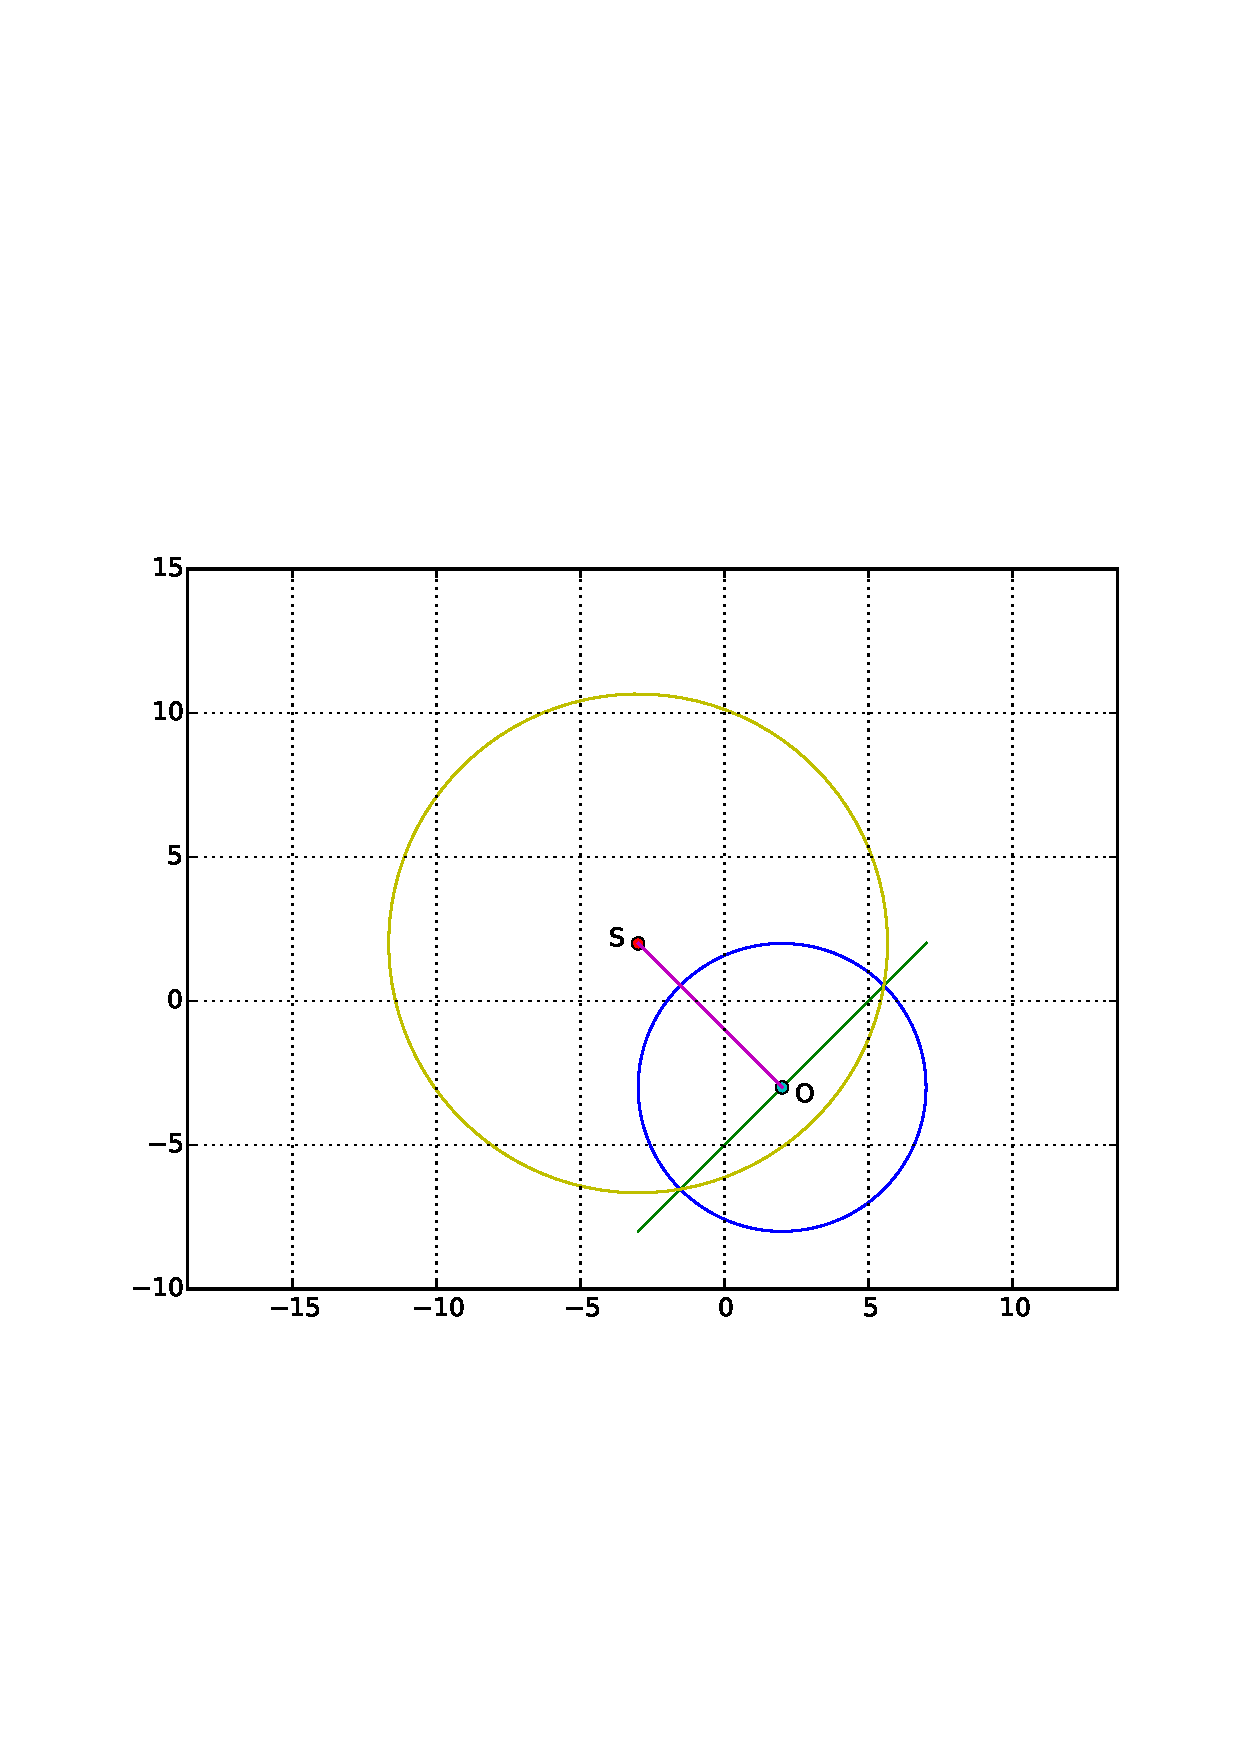
\includegraphics[width=\columnwidth]{./figs/ee16b1036}
\caption{ The diameter of circle with centre $O$ is a chord of the circle with centre $S$.}
\label{fig_36}	
\end{figure}
%

\begin{problem}
$P$ is the nearest point of the parabola $y^2=8x$ to the centre $C$ of the circle $x^2+\brak{y+6}^2=1$.Sketch the circle with centre $P$ and passing through $C$.
\end{problem}
\solution
Let $P$ be denoted by $\brak{2t^2,4t}$.  Let the centre of the circle $\brak{0,-6}$ be $O$. Then
%
\begin{equation}
OP^2 = (2t^2-0)^2+(4t+6)^2 = 4\brak{t^4+4t^2+12t+9}
\end{equation}
%
Differentiating $OP^2$ with respect to t and equating to 0 results in
\begin{align}
t^3+2t+3&=0\\
\Rightarrow (t+1)(t^2-t+3)&=0\\
\end{align}
yielding  $t=-1$.  Thus, $P$ is $\brak{2,-4}$ and $OP = 2\sqrt{2}$.  The equation of the desired circle is
%
\begin{equation}
\brak{x-2}^2 + \brak{y+4}^2 = 8
\end{equation}
%

\lstinputlisting{./codes/ee16b1037.py}
\renewcommand{\thefigure}{\theproblem.\arabic{figure}}
\begin{figure}[h]
\centering
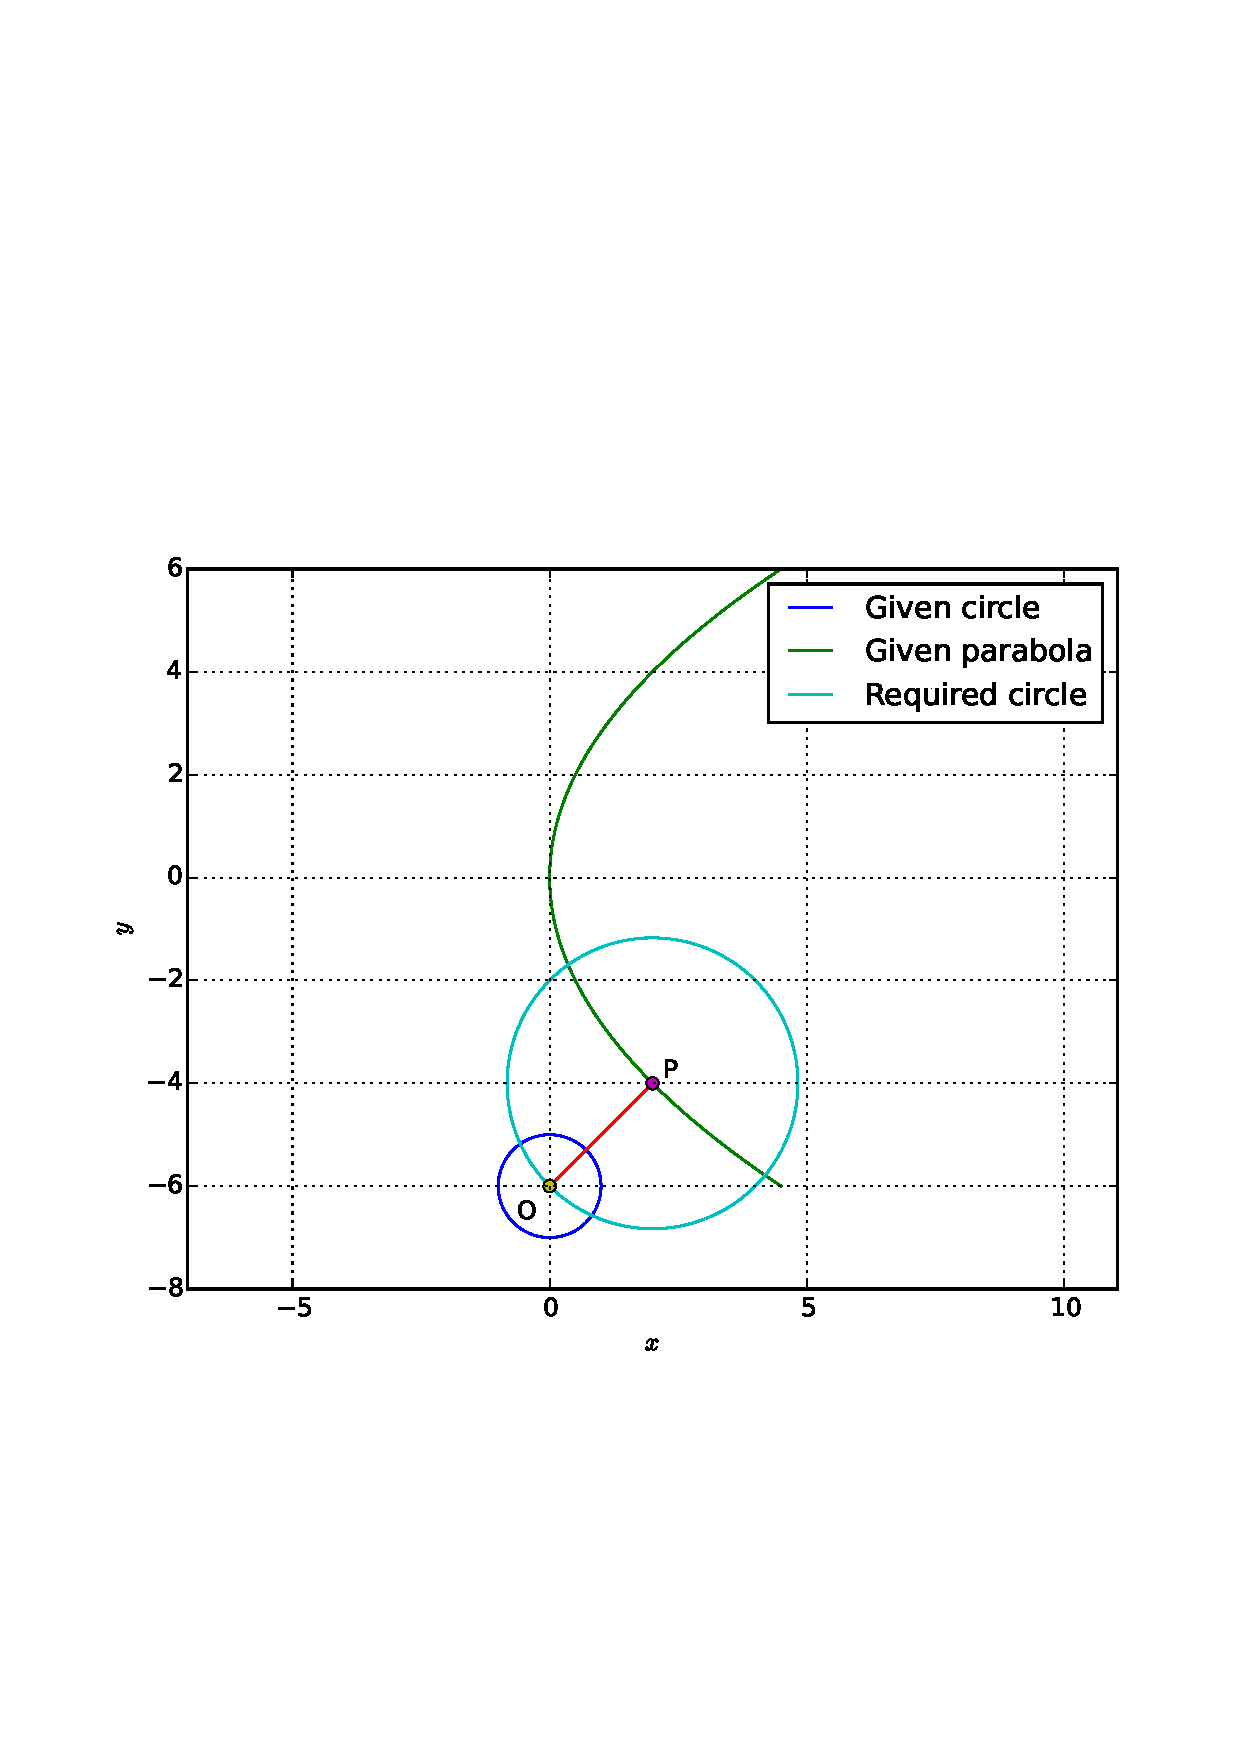
\includegraphics[width=\columnwidth]{./figs/ee16b1037a}
\caption{ Figures for the given problem}
%\label{fig_16}	
\end{figure}
%
\begin{figure}[h]
\centering
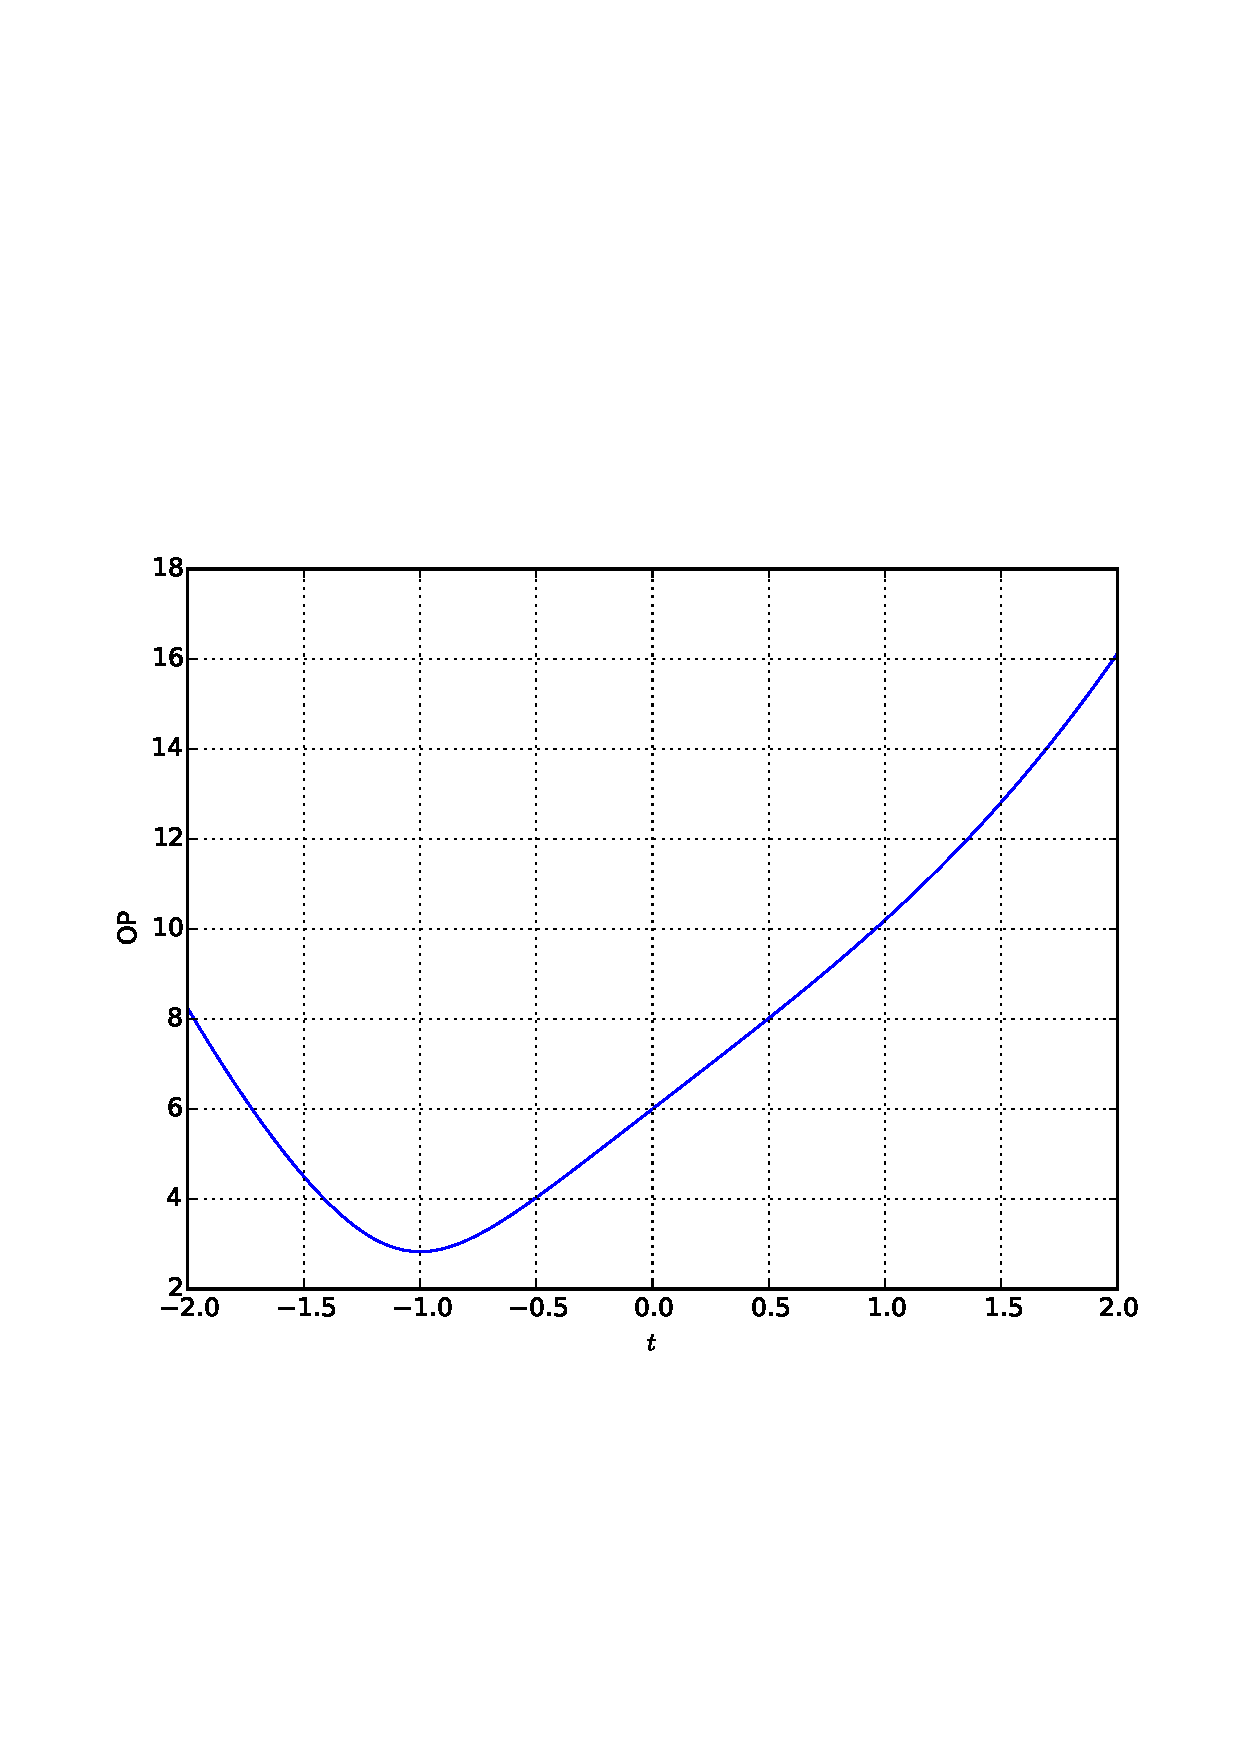
\includegraphics[width=\columnwidth]{./figs/ee16b1037b}
\caption{ $OP$ has a minimum at $t = -1$.}
%\label{fig_16}	
\end{figure}
\renewcommand{\thefigure}{\theproblem}
\begin{problem}
The length of the latus rectum of a hyperbola is 8 and the length of its conjugate axis is half the distance between its foci.  Sketch the hyperbola and find its eccentricity.
\end{problem}
\solution
Let the equation of the hyperbola be
%
\begin{align}
\frac{x^2}{a^2}- \frac{y^2}{b^2} = 1
\end{align}
%
Since the length of the latus rectum is 8,
%
\begin{equation}
\frac{2b^2}{a} =1
\end{equation}
%
The length of the conjugate axis is $2b$ and the distance between the foci is $2ae, e = \sqrt{1 + \frac{b^2}{a^2}}$, where $e$ is the eccentricity. Given that $2b = \frac{2ae}{2}$.
From the given information,
%
\begin{equation}
2b = \sqrt{a^2 + b^2}
\end{equation}
%
Since $a = 2b^2$, from the above equation, $b = \frac{\sqrt{3}}{2}$ and $a = \frac{3}{2}$. The eccentricity
%
\begin{equation}
e = \frac{2}{\sqrt{3}}
\end{equation}
%

The desired hyperbola is plotted in Fig. \ref{fig_38}.
\lstinputlisting{./codes/ee16b1038.py}
%
\begin{figure}[h]
\centering
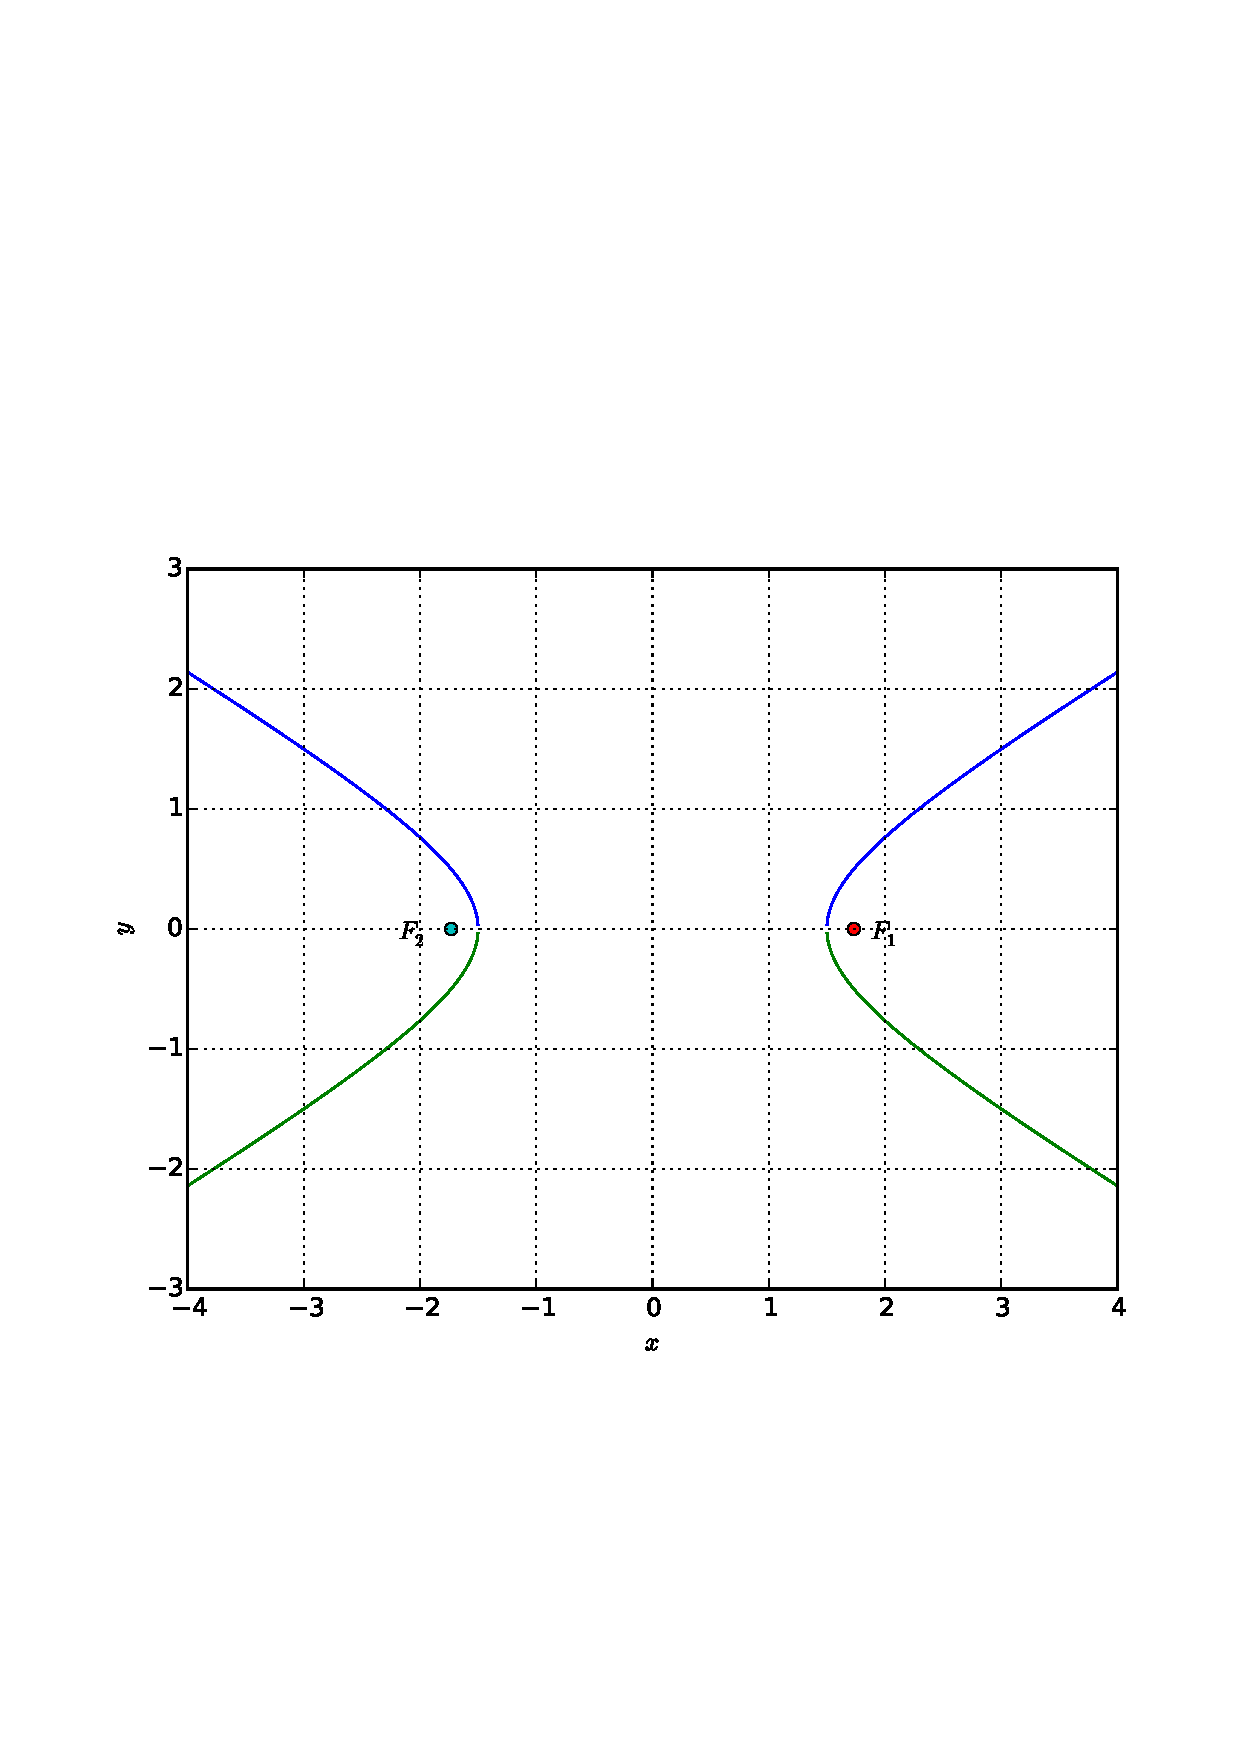
\includegraphics[width=\columnwidth]{./figs/ee16b1038}
\caption{ Foci at $F_1$ and $F_2$. Eccentricity $e = \frac{2}{\sqrt{3}}$}
\label{fig_38}	
\end{figure}
%
\begin{problem}
A wire of length 2 units is cut into two parts which are bent respectively to form a square of side $x$ units and a circle of radius of r units. Find $x$ if the sum of the areas of the square and the circle so formed is minimum.
\end{problem}
\solution
From the given information, adding the perimeters of the square and the circle,
%
\begin{equation}
4x + 2\pi r = 2 \Rightarrow 2x + \pi r = 1
\end{equation}
%
The sum of the areas of the square and circle is 
%
\begin{align}
A &= x^2 + \pi r^2 = x^2 +  \frac{\brak{1 - 2x}^2}{\pi}
\\
&= \frac{\brak{\pi + 4}x^2 -4x + 1}{\pi}
\\
&= \brak{1 + \frac4{\pi}}\cbrak{\brak{x - \frac{2}{\brak{\pi + 4}}}  + \frac{1}{\brak{\pi + 4}}- \brak{\frac{2}{\brak{\pi + 4}}}^2}
\end{align}
%
Thus, $A$ is minimum for $x = \frac{2}{\pi + 4}$. We obtain
%
\begin{equation}
r = \frac{1 - \frac{4}{4+\pi}}{\pi} = \frac{1}{\pi + 4} = \frac{x}{2}
\end{equation}
%
Let $P$ be denoted by $\brak{2t^2,4t}$.  Let the centre of the circle $\brak{0,-6}$ be $O$. Then
%
\begin{equation}
OP^2 = (2t^2-0)^2+(4t+6)^2 = 4\brak{t^4+4t^2+12t+9}
\end{equation}
%
Differentiating $OP^2$ with respect to t and equating to 0 results in
\begin{align}
t^3+2t+3&=0\\
\Rightarrow (t+1)(t^2-t+3)&=0\\
\end{align}
yielding  $t=-1$.  Thus, $P$ is $\brak{2,-4}$ and $OP = 2\sqrt{2}$.  The equation of the desired circle is
%
\begin{equation}
\brak{x-2}^2 + \brak{y+4}^2 = 8
\end{equation}
%

Fig. \ref{fig_39} plots $A$ with respect to $x$.
\lstinputlisting{./codes/ee16b1039.py}
%
\begin{figure}[h]
\centering
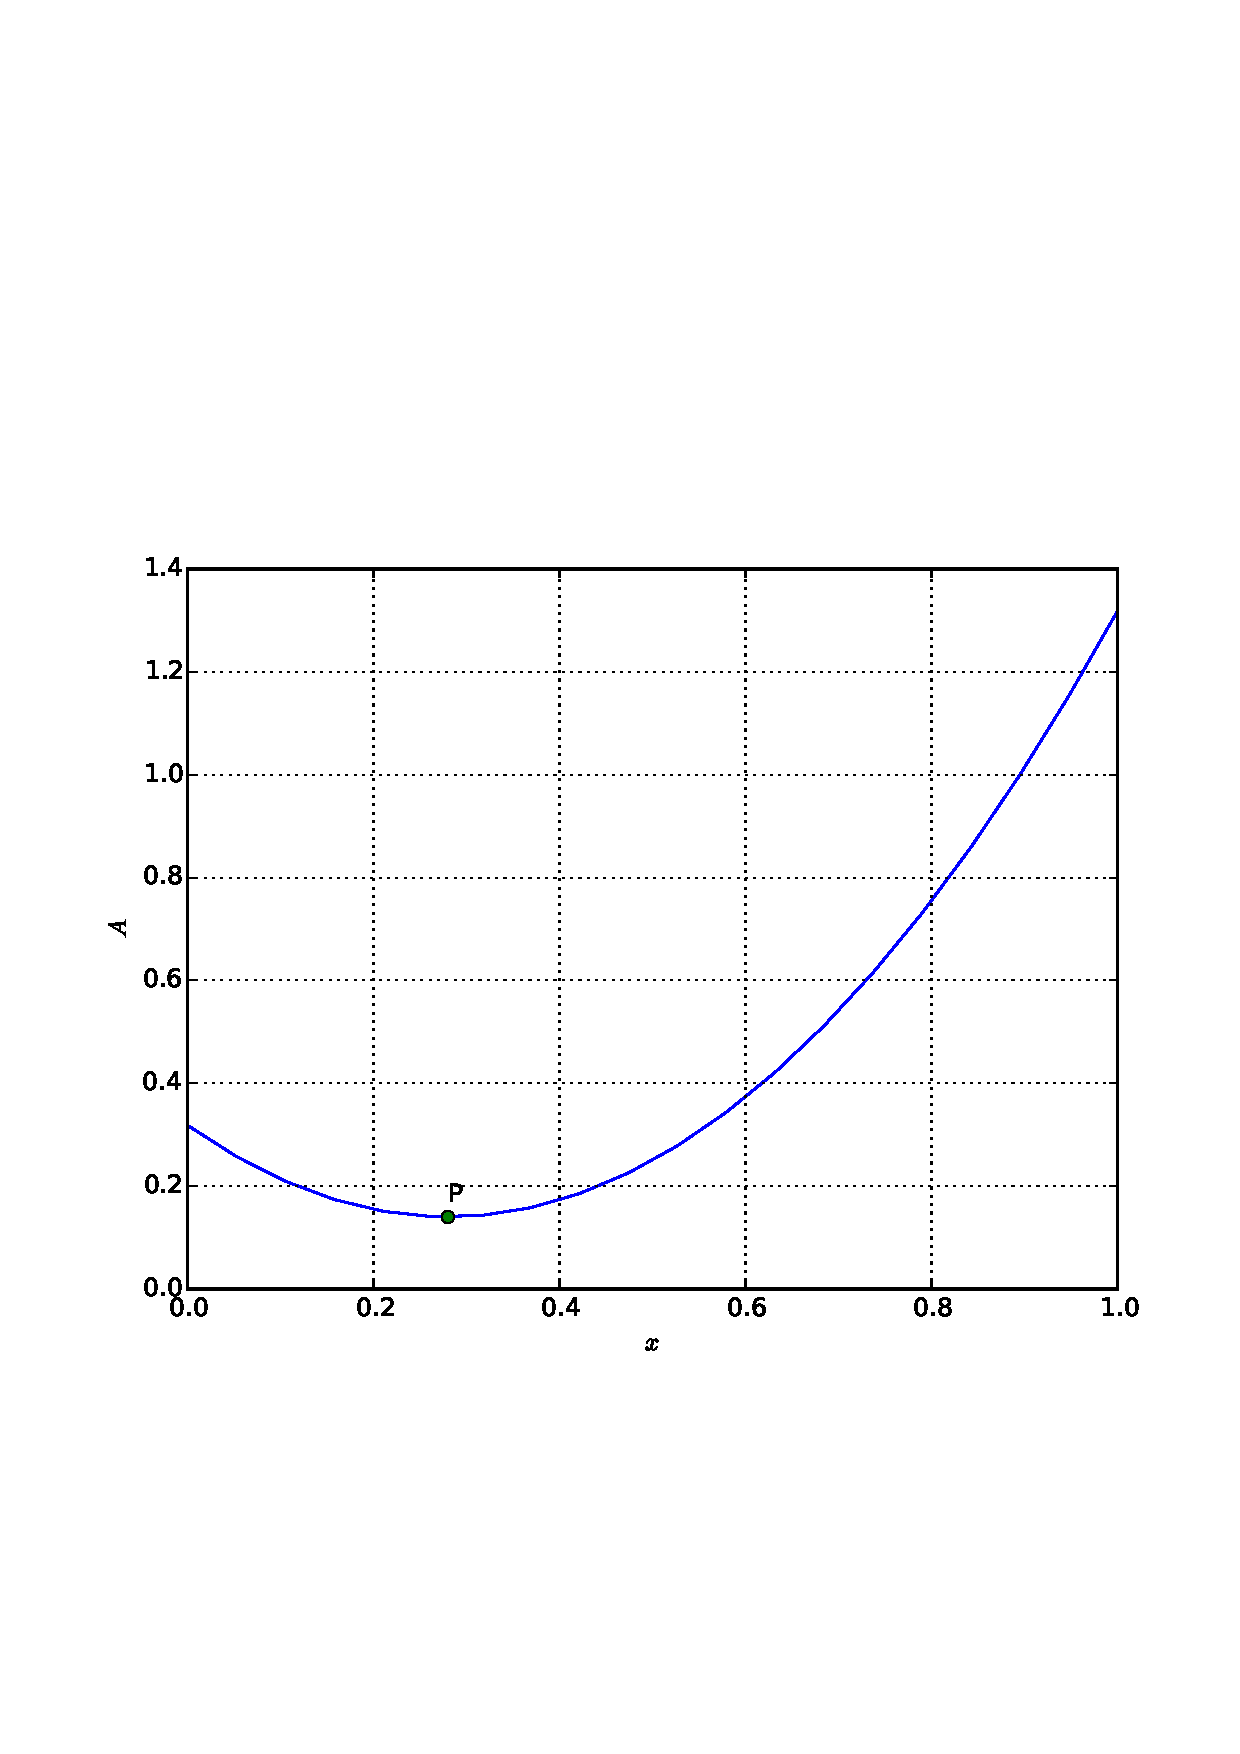
\includegraphics[width=\columnwidth]{./figs/ee16b1039}
\caption{ Area is minimum for $x = \frac{2}{\pi + 4}$}.
\label{fig_39}	
\end{figure}
%

\end{document}

